\chapter{Photon Detection System}
\label{ch:dp-pds}

The \dword{pds} of the \dune \dual module uses large-area cryogenic \dwords{pmt} coated with \dword{tpb} to detect the \SI{127}{\nm} light produced by argon scintillation. The \dwords{pmt} are installed on the cryostat floor, underneath the \dshort{tpc} transparent cathode, and view the entire \lar volume of one \dword{fd} module. The design described in this chapter builds on experience from several \lartpc{}s, and particularly from the \dword{wa105} and from the \dword{pddp} detectors at \dshort{cern}. 

The chapter is organised as follows. Sec.~\ref{sec:dp-pds-requirements} introduces the physics requirements to be met by the \dword{pds}, and additional opportunities offered by the system. Sec.~\ref{sec:dp-pds-overview} gives gives an overview of the \dword{pds} baseline design, together with the detector specifications to be satisfied. Secs.~\ref{sec:dp-pds-photosensors}--\ref{sec:dp-pds-calibration} describe in detail the \dword{pds} baseline design, and particularly the \dword{pds} photosensor system (Sec.~\ref{sec:dp-pds-photosensors}), the mechanical aspects (Sec.~\ref{sec:dp-pds-mechanics}),  the readout electronics (Sec.~\ref{sec:dp-pds-electronics}) and the calibration system (Sec.~\ref{sec:dp-pds-calibration}). Secs.~\ref{sec:dp-pds-simulation}--\ref{sec:dp-pds-performance} demonstrate how the PDS baseline design has been validated using detailed simulations (Sec.~\ref{sec:dp-pds-simulation} and \ref{sec:dp-pds-performance}) and experience from prototypes (Sec.~\ref{sec:dp-pds-prototypes}). Secs.~10-15 cover PDS project aspects, namely: quality control (Sec.~10), interfaces (Sec.~11), installation (Sec.~12), risks (Sec.~13), safety (Sec.~14), and high-level schedule and cost (Sec.~15). Finally, Sec.~16 discusses a limited number of alternatives to this baseline design.  

\section{Physics Requirements and Goals}
\label{sec:dp-pds-requirements}

The \dword{pds} of the \dune \dword{fd} provides information on three key detection aspects of the experiment:

\begin{enumerate}
\item Event (and sub-event) time reconstruction;
\item Event triggering;
\item Event energy reconstruction.
\end{enumerate}

As discussed below, these detection aspects enabled by the \dword{pds} affect the entire primary physics program of \dune: long-baseline neutrino oscillations, nucleon decay, and \dword{snb}. In the following, we list the scientific requirements the \dword{pds} will meet  (Sec.~\ref{subsec:dp-pds-requirements_requirements}), as well as additional scientific opportunities \dword{pds} offers (Sec.~\ref{subsec:dp-pds-requirements_opportunities}). Among requirements, we only list how \dword{pds} primarily affects the \dune primary physics program, namely: 
\begin{enumerate}
\item A capability or measurement uniquely provided by the \dword{pds};
\item A capability or measurement redundant with \dword{tpc} information, but where redundancy is considered essential;
\item A capability or measurement competitive with \dword{tpc} information.
\end{enumerate}

%%%%%%%%%%%%%%%%%%%%%%%%%%%%%%%%%%%%%%%%%%%%%%%%%%%%%%%%%%%%%%%%%%%%

\subsection{Scientific Requirements}
\label{subsec:dp-pds-requirements_requirements}

\subsubsection{Event fiducialization for non-beam events}

The accelerator complex for beam events provides absolute event time in the \dune \dword{tpc}, but the \dword{pds} must provide absolute event time for non-beam events. Event time reconstruction is necessary to determine the drift distance within the \dword{tpc}. This is essential for a number of reasons, particularly for defining a fiducial volume along the \dword{tpc} drift direction, which is the vertical one for \dword{dp}. The cosmic ray activity in one \dword{fd} module is of order \SI{0.05}{\Hz}, or about \SI{1e8}{\per(\Mtyr)}. Although smaller, the atmospheric neutrino event rate in one \dword{fd} module is also significant, of order \SI{1e5}{\per(\Mtyr)}. These rates can be compared with the background levels target for \dword{ndk} searches at \dune. For the \dword{ndk} channels where \dune can provide the best sensitivities, the goal is to operate in nearly background-free conditions even after an exposure of several years, that is, with background levels of order \SI{10}{\per(\Mtyr)} or less. Hence, the cosmic ray activity must be suppressed by at least seven orders of magnitude to enable optimal \dword{ndk} searches. \dword{pds} information is essential to reach the required levels of suppression of cosmic ray-induced (and atmospheric neutrino-induced) backgrounds. Because most cosmic ray activity will enter from the top of the detector, a \dword{ndk} candidate must be fully contained within the detector. For the most relevant direction, namely the vertical one, the fiducial requirement can only be imposed if \dword{pds} information is available. Because this capability is uniquely provided by the \dword{pds} and because it critically affects the \dword{ndk} program, {\bf we consider event fiducialization of \dword{ndk} candidates to be the most important requirement of the \dword{pds}}. High signal efficiency is critical in rare event searches like \dword{ndk}, so {\bf we require a $\boldsymbol{>90\%}$ efficient event time determination via the \dword{pds} throughout the \dword{tpc} active volume for \dword{ndk} signal events}. \dword{ndk} event fiducialization may be prevented not only if \dword{ndk}-induced \dshort{lar} scintillation flashes are undetected, but also if the \dword{pds} detects spurious \dshort{lar} scintillation flashes within the same event window, uncorrelated with the \dword{ndk} activity. Additional flashes are produced, typically, by radiologically-induced detector activity. In this case, an ambiguity in the drift time determination of the \dword{ndk} may arise, and the correct (\dword{ndk}-induced) flash must be associated to the event. Hence, {\bf we also require a $\boldsymbol{>90\%}$ \dword{ndk} flash purity among all reconstructed \dword{ndk}-like flashes within the same \dword{ndk} event readout window}. Similarly, the \dword{pds} is also needed to determine the full containment of atmospheric neutrino interactions in \dune.
 
\subsubsection{Supernova burst triggering}

A burst of several hundred neutrino interactions per \dune \dword{fd} module is expected over a timescale of about \SI{10}{\s} from a core-collapse supernova at a \SI{10}{\kilo\parsec} distance from the Earth, near the center of our galaxy. As the \dword{snb} interaction rate scales as $1/r^2$, where $r$ is the supernova distance from us, \dword{snb} detection at \dune is in principle possible up to distances of order \SI{50}{\kilo\parsec}. This would be the case for an \dword{snb} occurring in the Large Magellanic Cloud, for example. The dominant neutrino interaction channel in \dune is the \dword{cc} electron neutrino interaction on an argon nucleus, with typical deposited energies from electrons and nuclear de-excitation gammas of order \SI{20}{\MeV}, producing short tracks throughout the \dword{tpc} active volume.

In \dune, one can in principle trigger on \dwords{snb} using either \dword{tpc} or \dword{pds} information. In both cases, the trigger scheme exploits the time coincidence of multiple signals (\dword{tpc} stubs or \dword{pds} optical clusters\footnote{Throughout this chapter, we use the term "optical flash" for the process of scintillation light production in \dshort{lar}. We use "optical hit" to identify a reconstructed optical signal in a single photo-detector channel. We use the term "optical cluster" to name the reconstructed object given by a collection of optical hits seen by separate photo-detectors and that are correlated in time/space.}) over a timescale matching the SN luminosity time evolution. In the case of an \dword{snb} trigger being generated, the data acquisition system would write to disk the full (non-zero-suppressed) detector information for a time range spanning several tens of seconds surrounding the trigger timestamp. Considering the rarity of \dwords{snb} in our galactic neighbourhood, and given the importance of \dword{snb} detection, we consider it essential to develop both a redundant and a highly efficient \dword{snb} triggering scheme in \dword{dune}. Concerning redundancy, {\bf we require that the \dune \dword{fd} may trigger on an \dword{snb} independently using \dword{tpc} or \dword{pds} information}, hence minimizing \dword{snb} inefficiencies stemming from downtime or malfunctioning of the \dword{tpc}, the \dword{pds}, or their associated trigger schemes. As for trigger efficiency, {\bf we require the \dword{pds} alone to be able to trigger with $\boldsymbol{>90\%}$ efficiency on an \dword{snb} at a \SI{20}{\kilo\parsec} distance from Earth}, hence up to distances covering the entire Milky Way. Considering the very large amount of detector information being generated by an \dword{snb} trigger, we also require that the \dword{snb} trigger efficiency be reached for a {\bf fake trigger rate not exceeding \SI{1}{\per month}}.

\subsubsection{Scintillation-based calorimetry}

The most important physics goal of the \dune \dword{fd} is to carry out a comprehensive program of neutrino oscillation measurements using \numu and \anumu beams from Fermilab. Because of this, the \dune \dword{fd} performance in terms of neutrino energy reconstruction and neutrino flavour classification is of paramount importance. As detailed in this volume, the \dword{tpc} should provide a 10--15\% neutrino energy resolution for \nue \dword{cc} interactions in the few-GeV energy range, using charge information alone. At these energies, however, the \dword{pds} will also detect thousands of PEs. Thus, a competitive calorimetric measurement of the event energy can also, in principle, be obtained using the light intensity detected by the \dword{pds}, if spatial non-uniformities in \dword{pds} response can largely be corrected for. {\bf We require the \dword{pds} alone to be able to reconstruct the neutrino energy of a few-GeV electron neutrino \dword{cc} interaction with 20\% \dword{rms} resolution or better}, thus providing a measurement competitive to the \dword{tpc}-based one. Such an independent and competitive energy measurement would also be useful as a risk mitigation measure for degraded \dword{tpc} performance. The \dword{tpc}- and \dword{pds}-based energy measurements may be combined, possibly providing better energy resolution than \dword{tpc} alone. We give two arguments supporting this possibility. On one hand, the charge and light signals may be combined to reduce electron-ion recombination fluctuations, ensuring a more compensating \dword{lar} calorimeter response. On the other hand, charge and light readout planes are located at opposite detector ends in the \dword{dp} design, providing maximal complementarity between the two sub-systems. Neutrino interactions occurring near the light readout at the bottom of the cryostat will be maximally affected by electron attachment of the charge signal, while they will have the highest light detection probabilities possible. The situation is reversed for neutrino interactions near the charge readout plane. The \dword{pds} may provide a competitive energy measurement not only for beam neutrinos, but also at lower energies, particularly for \dword{snb} neutrinos. For a discussion of why an accurate energy measurement is beneficial also for \dword{snb} events, see Sec.~\ref{subsubsec:dp-pds-requirements_attachment}.

%%%%%%%%%%%%%%%%%%%%%%%%%%%%%%%%%%%%%%%%%%%%%%%%%%%%%%%%%%%%%%%%%%%%

\subsection{Additional Scientific Opportunities}
\label{subsec:dp-pds-requirements_opportunities}

\subsubsection{Electron attachment correction for the charge-based energy measurement in non-beam events}
\label{subsubsec:dp-pds-requirements_attachment}

Given the maximum drift distance of \dpmaxdrift in the \dual \dword{tpc} and assuming a (minimally-required) \SI{3}{\ms} electron lifetime, the charge could be attenuated by more the one order of magnitude along drift due to electron attachment on electro-negative impurities. If left uncorrected, electron attachment would therefore cause great deterioration in the charge-based energy measurement in such relatively short electron lifetimes. Because of the longer drift distance, this effect is much more dramatic in the \dword{dp} than the \dword{sp}. For non-beam events, the only possible way of correcting for the electron attachment is through \dword{pds}-based event timing\footnote{This is true for a single physics event (e.g., a neutrino interaction) per \dword{tpc} event. Other than background flashes, the association between \dword{tpc} tracks and \dword{pds} flashes has no ambiguities.}. This will be exploited in \dune to better discern, for example, the spectral features in the energy spectrum of the \dword{snb} flux. An improved charge-based energy measurement would improve both the determination of the pinched-thermal spectral parameters of the progenitor, and the detection of the sharp, time-dependent spectral features from collective neutrino oscillations. A similar argument applies to the charge-based energy measurement in the study of atmospheric neutrino oscillations, where good neutrino energy reconstruction is also very important.

\subsubsection{Event timing in high multiplicity supernova burst events}

The early time distribution carries important information for core-collapse stellar models, which has not been observed thus far. The first neutrino release after core bounce is the \nue-rich neutronization burst, lasting about \SI{10}{\ms}. For a supernova at \SI{10}{\kilo\parsec} distance, several tens of interactions induced by the neutronization flux should be detected in one \dword{fd} module. In other words, the mean interval between successive neutrino interactions should be less than \SI{1}{\ms} in this case. For closer supernovae, information at even earlier (pre-bounce) times may be studied during the core infall phase. A \SI{1}{\ms} wide notch in the luminosity curve may be visible, corresponding to neutrino trapping in the ultra-dense matter. Such timescales can be compared with the typical time resolutions obtained with \dword{tpc} and \dword{pds} information. For \dword{dp} \dword{tpc} and for a \SI{1.6}{mm/\micro\s} electron drift velocity, the drift time can be as large as \SI{7.5}{\ms}, with foreseen readout windows of \dpreadout. Considering the uniform spatial distribution of neutrino interactions in the \dword{tpc}, the intrinsic absolute time resolution expected in this case is of order $\dpreadout/\sqrt{12}\simeq \SI{5}{\ms}$. The \dword{tpc}-based time resolution is therefore not sufficient to resolve these early time features, even in the case of sufficient neutrino statistics. On the other hand, the \dword{pds} may reconstruct one flash per \dword{snb} neutrino interaction at \SI{1}{\micro\s}-scale time resolution or more. Hence, \dword{pds}-based timing is definitely an added value for a nearby supernova.

\subsubsection{Improved event identification via scintillation-based Michel electron tagging}

There is another physics case where the \dword{pds} may detect more than one physics-induced flash per \dword{tpc} event\footnote{We use the qualifier 'physics-induced' to distinguish those light flashes from the ones induced by radiological or cosmogenic activity in the detector or by electronics noise.}. This can happen in the presence of particle decays in the final state of an event of interest, such as a neutrino interaction or a nucleon decay. In this case, multiple, correlated sub-events may be separated in time. Michel electron tagging from muon decay at rest is the most obvious opportunity for sub-event identification using \dword{pds} timing. Approximately one million scintillation photons are produced in the liquid argon per Michel electron. In addition, the timescale of muon decay is long, comparable to the timescale of the slow component of argon scintillation light. Although Michel electrons can also be identified through \dword{tpc} track imaging, in some event topologies,  \dword{pds} may outperform the \dword{tpc}, for example where the muon and electron tracks are nearly parallel. In summary, the \dword{pds} may better identify the event final state than \dword{tpc}-only information. Considering the large fraction of $\mu^-$ capture on argon (about 75\%), Michel electron tagging also provides valuable $\mu^-/\mu^+$ separation. The latter can, in turn, provide separation between muon neutrinos and antineutrinos. 

\section{Design Overview}
\label{sec:dp-pds-overview}

The \dual \dword{pds} is optimized for the physics program of the full-size \dune \dual detector. Phenomena leading to interactions in the \dword{dune} detectors and to be studied span several orders of magnitude of energy scale, from a few \si{MeV} to several \si{GeV}, with commensurate range in light yield. In particular, low-energy signals like \dword{snb} neutrinos and proton decay, impose more stringent requirements on \dword{pds} performance than the primarily higher energy, beam-synchronous, neutrino oscillations physics.

%A number of scientific and technical choices and issues impact the \dual \dword{pds}  and \single \dword{pds}  in a similar way, so the consortia for these two systems cooperate closely.  %See \voltitlespfd{}, Chapter 5 for details on the \single \dword{pds}.

%%%%%%%%%%%%%%%%%%%%%%%%%%%%%%%%%

\subsection{Scintillation Light Production in the \dual Detector Module}
\label{sec:dp-pds-overview_scintillation}

\dual \dword{pds} detects light produced from two sources: the scintillation process originated by ionizing particles propagating in the liquid argon (usually referred to as the S1 signal) and by the electroluminescence process due to drift electrons extracted from the liquid phase and accelerated in the argon vapor at the top of the cryostat (usually referred to as the S2 signal). Charge readout anode planes instrument the top while photodetectors are at the bottom of the cryostat. The interplay between the charge and light from an event enables pattern recognition and measuring the energy of interactions.

Ionizing radiation in liquid noble gases leads to the formation of excimers in either singlet or triplet states, which decay radiatively to the dissociative ground state with characteristic S1 fast and slow lifetimes (fast is approximately \SI{6}{ns} and slow approximately \SI{1.3}{$\mu$s} in \lar with the so-called second continuum emission spectrum peaked at the wavelength of approximately \SI{127}{nm}, \SI{126.8}{nm} with a full width at half maximum of \SI{7.8}{nm} \cite{Heindl}). This prompt and relatively high-yield (about \num{40000} photons per \si{MeV} at zero \efield) of \SI{127}{nm} scintillation light is exploited in an \lartpc (both \dshort{dp} and \dshort{sp}) to provide the absolute time ($t_0$) of the ionization signal collected at the anode, thereby providing the absolute value of the drift coordinate of fully contained events and a prompt signal used for triggering. Figure~\ref{fig:dppd_6_0} shows the light production mechanism in \lar.

\begin{dunefigure}[A sketch depicting the mechanism of light production in argon.]{fig:dppd_6_0}
{A sketch depicting the mechanism of light production in argon.}
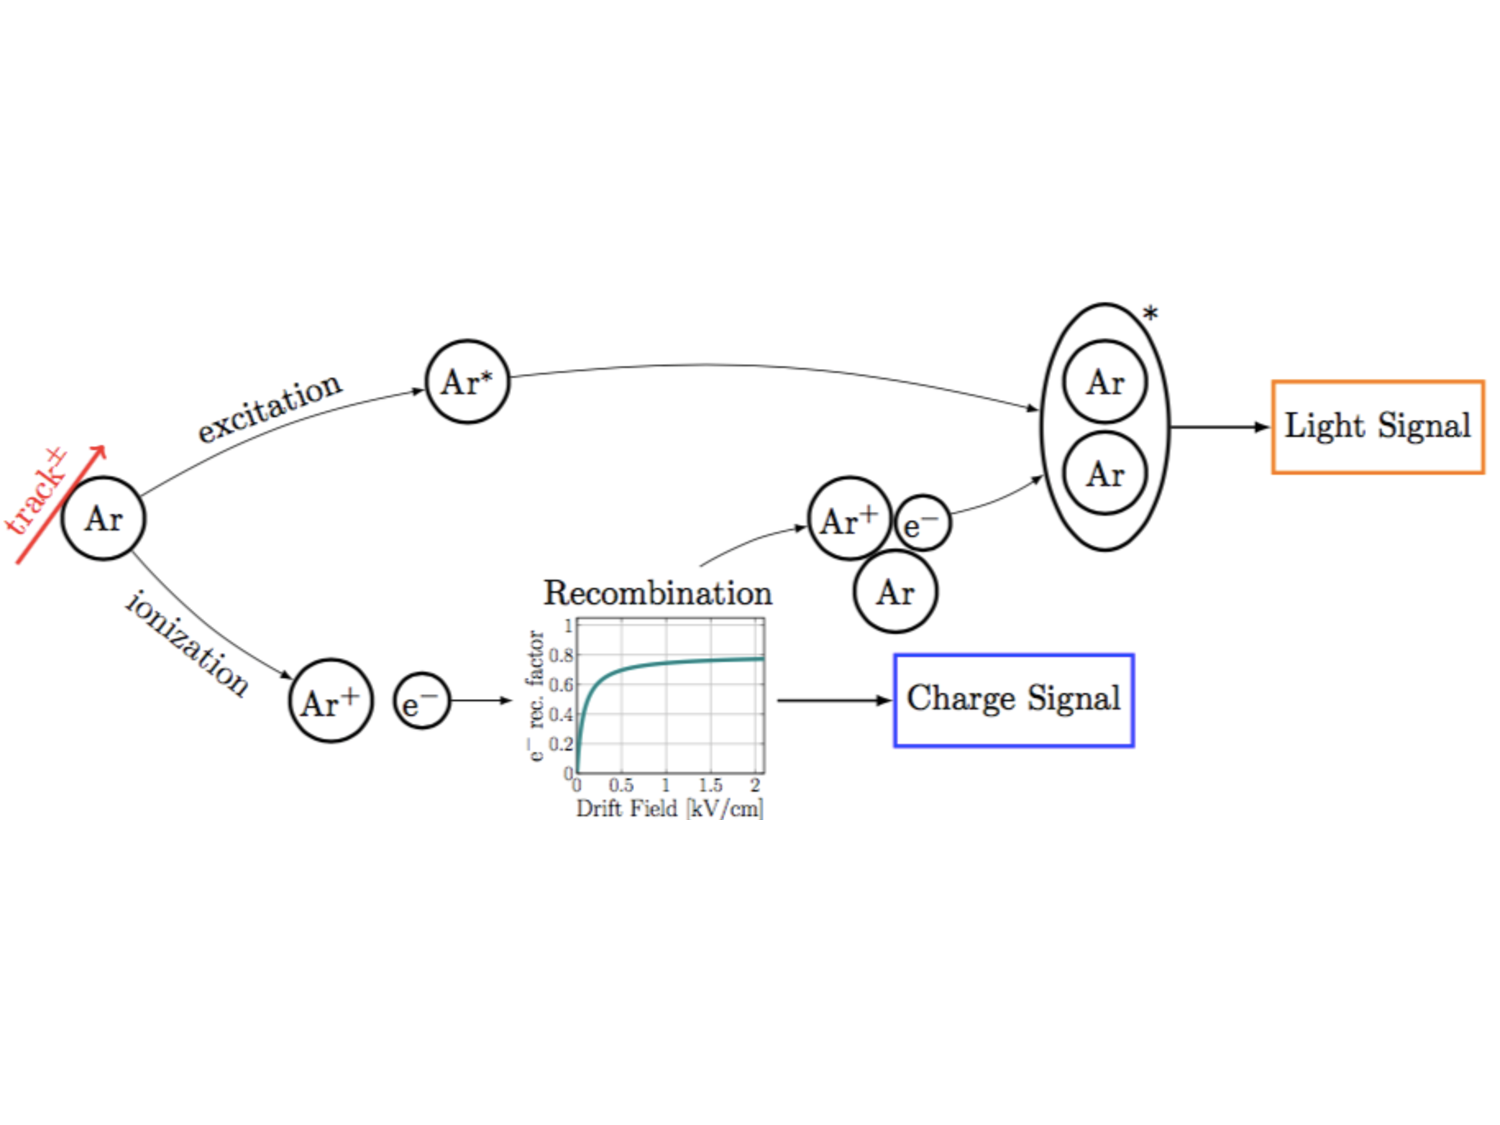
\includegraphics[width=0.95\textwidth]{dppd_6_0}
\end{dunefigure}

The secondary scintillation in the argon gas (i.e., the vapor phase) is unique to the \dpmod technology. It is the luminescence in gas caused by accelerated electrons in the \efield and in the \dword{lem} anode through Townsend amplification. The S2 signal provides information on the drift time and amount of ionization charge, thus supplementing information from the charge readout on the anode plane. For a given argon gas density, the number of S2 photons is proportional to the number of electrons, the \efield, and the length of the drift path in gas covered by the electrons. In an extraction field of \SI{3.0}{kV/cm} in gas, one electron generates about \num{100} downward-moving photons that cross the liquid argon surface \cite{Lux:2018zwd}. The time scale of S2 reflects the extraction time of original ionization from the liquid phase into the gas phase. Therefore, for about \SI{0.5}{kV/cm} drift \efield, this time scale is of the order of hundreds of microseconds. The time between the occurrence of the primary scintillation light and the secondary scintillation light is equivalent to the drift time of the electrons from the ionization coordinate to the \lar surface. This provides an accurate determination of the drift time in the active volume and, hence, a correction tool for the electron attachment (and the associated energy measurement).  


%The chapter begins with an overview of the system in Section~\ref{sec:fddp-pd-1}. Section~\ref{sec:fddp-pd-2} describes the photosensors, namely \dwords{pmt} %tubes  
%and the related \dword{hv} system, wavelength shifters and light collectors. The mechanics associated with the \dwords{pmt} is described in Section~\ref{sec:fddp-pd-3}, and the readout electronics in~\ref{sec:fddp-pd-4}. Section~\ref{sec:fddp-pd-5} details the photon calibration system to monitor the \dword{pmt} gain and stability. Then, the \dword{pd} performance is described in Section~\ref{sec:fddp-pd-6}, and the operations in Section~\ref{sec:fddp-pd-7}. Interfaces with other subsystems are described in Section~\ref{sec:fddp-pd-8}. Section~\ref{sec:fddp-pd-9} includes the installation, integration and commissioning plans. The \dword{qc} procedures are outlined in Section~\ref{sec:fddp-pd-10}. The main safety issues to consider are specified in Section~\ref{sec:fddp-pd-11}. To finish, the management and organization is described in Section~\ref{sec:fddp-pd-12}.

%%%%%%%%%%%%%%%%%%%%%%%%%%%%%%%%%
\subsection{Detector Sub-systems and Layout}
\label{sec:dp-pds-overview_layout}

The baseline design of the light collection system calls for \SI{20.3}{cm} (\SI{8}{in}) diameter cryogenic \dwords{pmt} from Hamamatsu Photonics\footnote{Hamamatsu Photonics\texttrademark{}, \url{http://www.hamamatsu.com/resources/pdf/etd/LARGE_AREA_PMT_TPMH1286E.pdf}} (model R5912-MOD20) distributed uniformly on the floor (bottom) of the cryostat and electrically shielded from the bottom cathode plane. Other \dword{pmt} manufacturers being considered include Electron Tubes Limited~\footnote{Electron Tubes Ltd\texttrademark{}, \url{http://www.electron-tubes.co.uk//}} and HZC~\footnote{HZC Photonics\texttrademark{}, \url{http://hzcphotonics.com/en_index.html}.}. According to the baseline design, \dpnumpmtch \dwords{pmt}, approximately \num{1} per \si{m$^2$}, will be installed. The outline of the \dword{dpmod} is shown in Figure~\ref{fig:dppd_3_1}.

\begin{dunefigure}[The \dword{dpmod} (partly open)]{fig:dppd_3_1}
{The \dword{dpmod} (partly open) with cathode, \dwords{pmt}, \dword{fc}, and anode plane with chimneys.}
%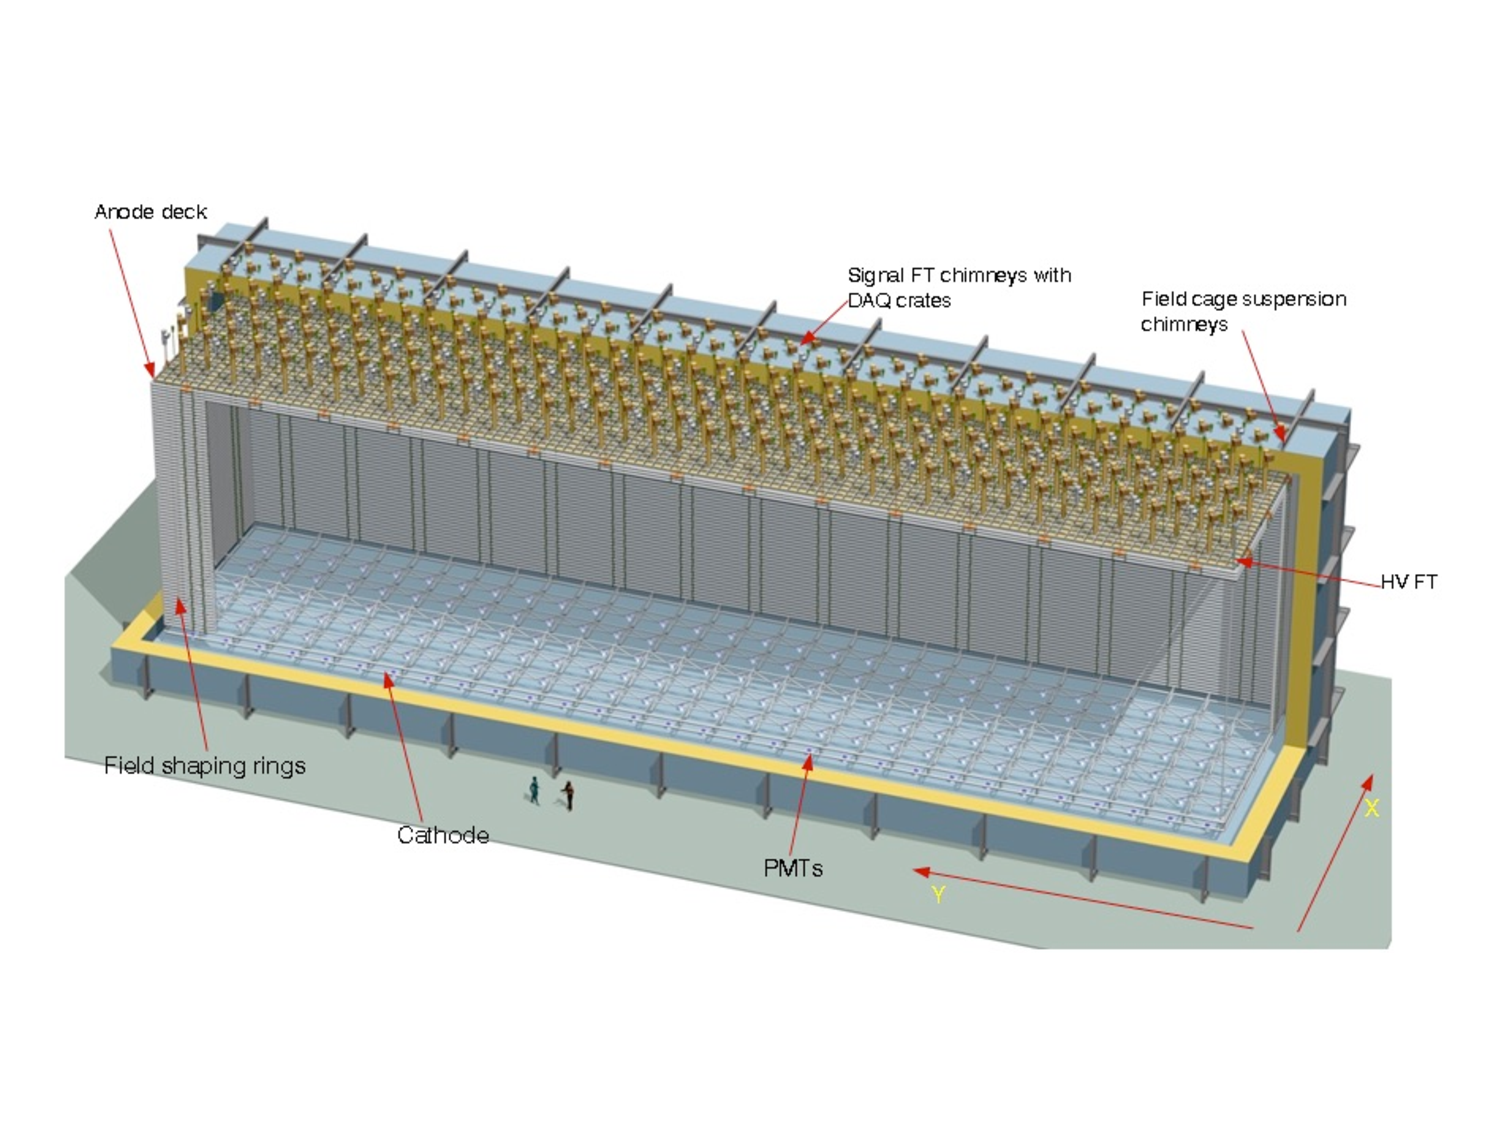
\includegraphics[width=0.95\textwidth]{dppd_3_1}
%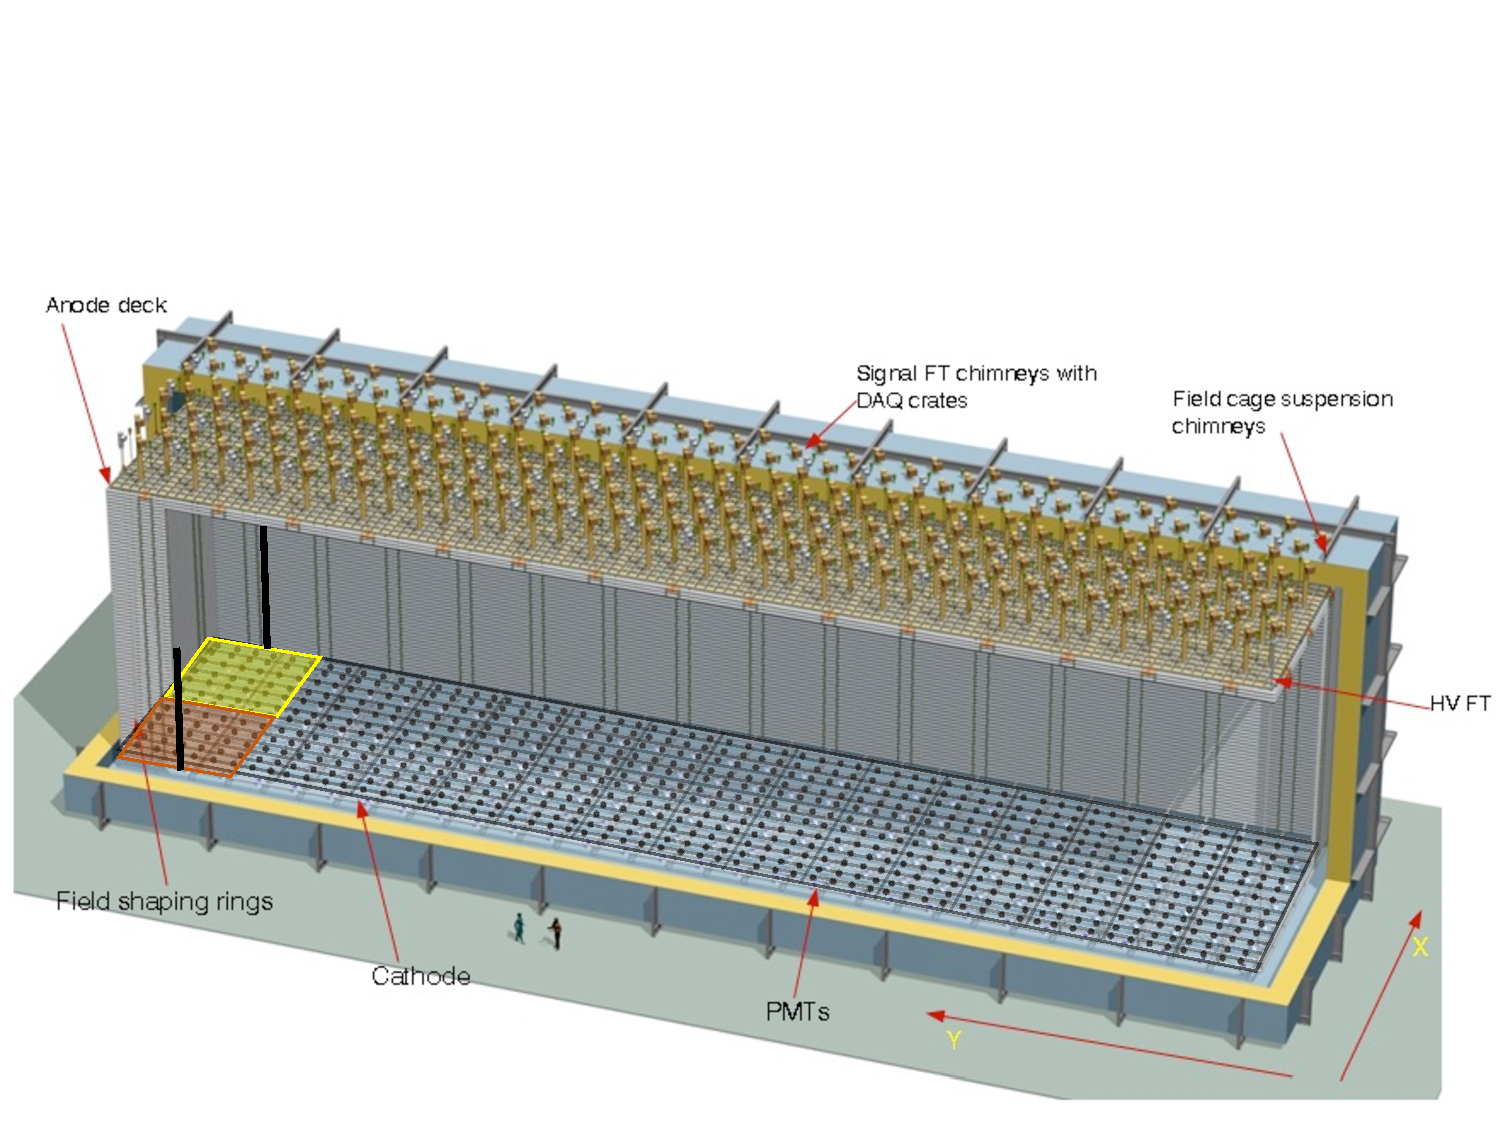
\includegraphics[width=0.95\textwidth]{dppd_1_1_v2}
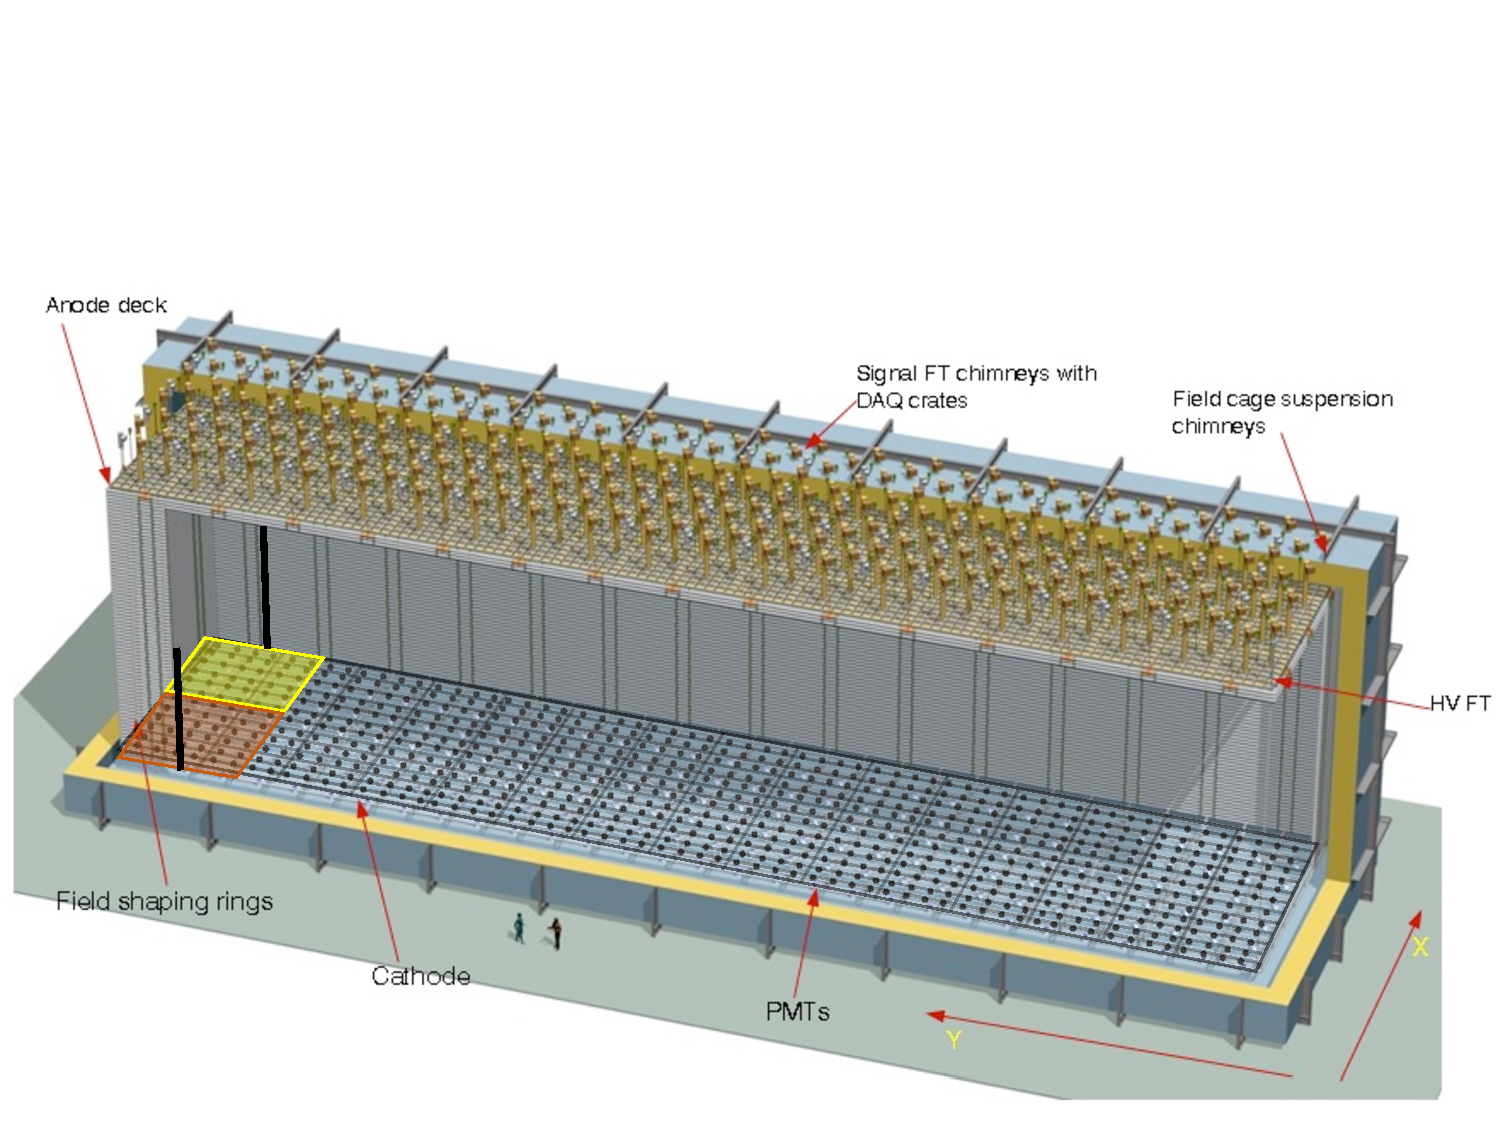
\includegraphics[width=0.95\textwidth]{dppd_1_1_v3}
\end{dunefigure}

The \dwords{pmt} are individually powered to values between \num{1.5} to \num{2.0} \si{\kV} to separately adjust the \dword{pmt} gains. The Hamamatsu R5912 \dwords{pmt} are not sensitive to the \SI{127}{nm} scintillation light, so a wavelength shifter is required. A thin layer of \dword{tpb}~\cite{tpb} coating is applied directly on the \dword{pmt} window by evaporation. Section~\ref{sec:dp-pds-photosensors} describes the photosensor system.

The \dpnumpmtch \dwords{pmt} are individually attached to the cryostat floor \SI{1.02}{m} apart in both directions, via a \dword{pmt} support structure that counteracts the \dword{pmt} buoyancy. In order to enhance the light collection and to improve the photon detector response uniformity throughout the entire \dword{tpc} active volume, \dword{tpb} coated reflector/\dword{wls} panels will be installed on the top half of the \dword{fc} inner surfaces. Considering the linear relationship between the number of \dwords{pmt} and the detected light yield, and the mild dependence of the \dword{pds} physics performance on light yield and channel granularity, the optimization process that resulted in this baseline design can be considered very robust. The mechanical aspects of the \dword{pmt} support structures and the reflector/\dword{wls} assemblies are described in Section~\ref{sec:dp-pds-mechanics}.

The front-end \dword{pmt} base circuit for reading the photo-electron signals relies on a positive \dword{hv} supplied to the \dword{pmt} anode and on a grounded photo-cathode. A single cable for each \dword{pmt} carries both power and signal. \dword{hv} and signal splitters located outside the cryostat separate the fast \dword{pmt} response signal from the positive \dword{hv} with capacitive decoupling. The \dword{pds} readout electronics is described in Section~\ref{sec:dp-pds-electronics}.

A photon calibration system is required to determine the \dword{pmt} gain and to monitor the stability of the \dword{pmt} response. The LED-driven fiber calibration system of the \dword{pds} is described in Section~\ref{sec:dp-pds-calibration}. 

The basic unit of installation/operation is called a sector. The sectors are indicated as transparent red and yellow panels in Figure~\ref{fig:dppd_3_1}. One \dual \dword{pds} sector is \SI{6}{\m} $\times$ \SI{6}{\m} and houses \num{36} \dwords{pmt}. A total of \num{20} sectors will be installed in the detector. A single \dword{hv} cable per \dword{pmt} will be installed in the cryostat.
%The cables from the \dword{pmt} locations (RG303/U) will run in bundles at the cryostat floor to either side. The short cables attached to the \dword{pmt} bases will be connected to these long cables during the \dword{pmt} installation at the cryostat floor. The long cables from each sector will be bundled and will run through a cable tray along the \SI{12}{\m} side wall to the top of the cryostat. 
The cable trays for the two sectors in Figure~\ref{fig:dppd_3_1} are indicated as black vertical lines.
%The single cable density is approximately \SI{50}{\g/\m}. The cable length at the cryostat floor will be \SI{9}{\m} (determined by the farthest \dwords{pmt}), the side wall length is \SI{12}{\m}, and the additional average cable length per \dword{pmt} is estimated to be \SI{4}{\m}. Therefore, the overall cable length per \dword{pmt} is \SI{25}{\m}. This corresponds to approximately \SI{2}{\kg/\m} load on the cable trays on the side walls (a total of \SI{24}{\kg} assuming a cable density of \SI{50}{\g/\m}) per sector, also including the \num{6} calibration fibers. 

The high voltage cables will penetrate a feedthrough flange and end with SHV connectors, with the calibration fibers also penetrating a feedthrough flange and end with SMA connectors. One DN250 flange is used per sector of \dual \dword{pds}. One flange will house \num{36} SHV and \num{6} SMA connections. The \dual \dword{pds} design will have \num{20} penetrations on the cryostat roof, one per sector. 

The high voltage and signal crates will be at a density of one per sector for a total of \num{20} \dword{hv}/signal racks on the cryostat roof. Figure~\ref{fig:dppd_1_2} illustrates the layout of the feedthroughs and the \dword{hv}/signal/calibration racks for four sectors. The racks will contain the \dword{hv} crates, \dword{hv}/signal splitters, the \dword{utca} crates for the front-end electronics, and the calibration LED driver and the associated electronics for \num{36} \dwords{pmt}.

\begin{dunefigure}[The sketch of the cryostat roof layout for \dual \dword{pds} penetrations.]{fig:dppd_1_2}
{The sketch of the cryostat roof layout for \dual \dword{pds} penetrations.}
%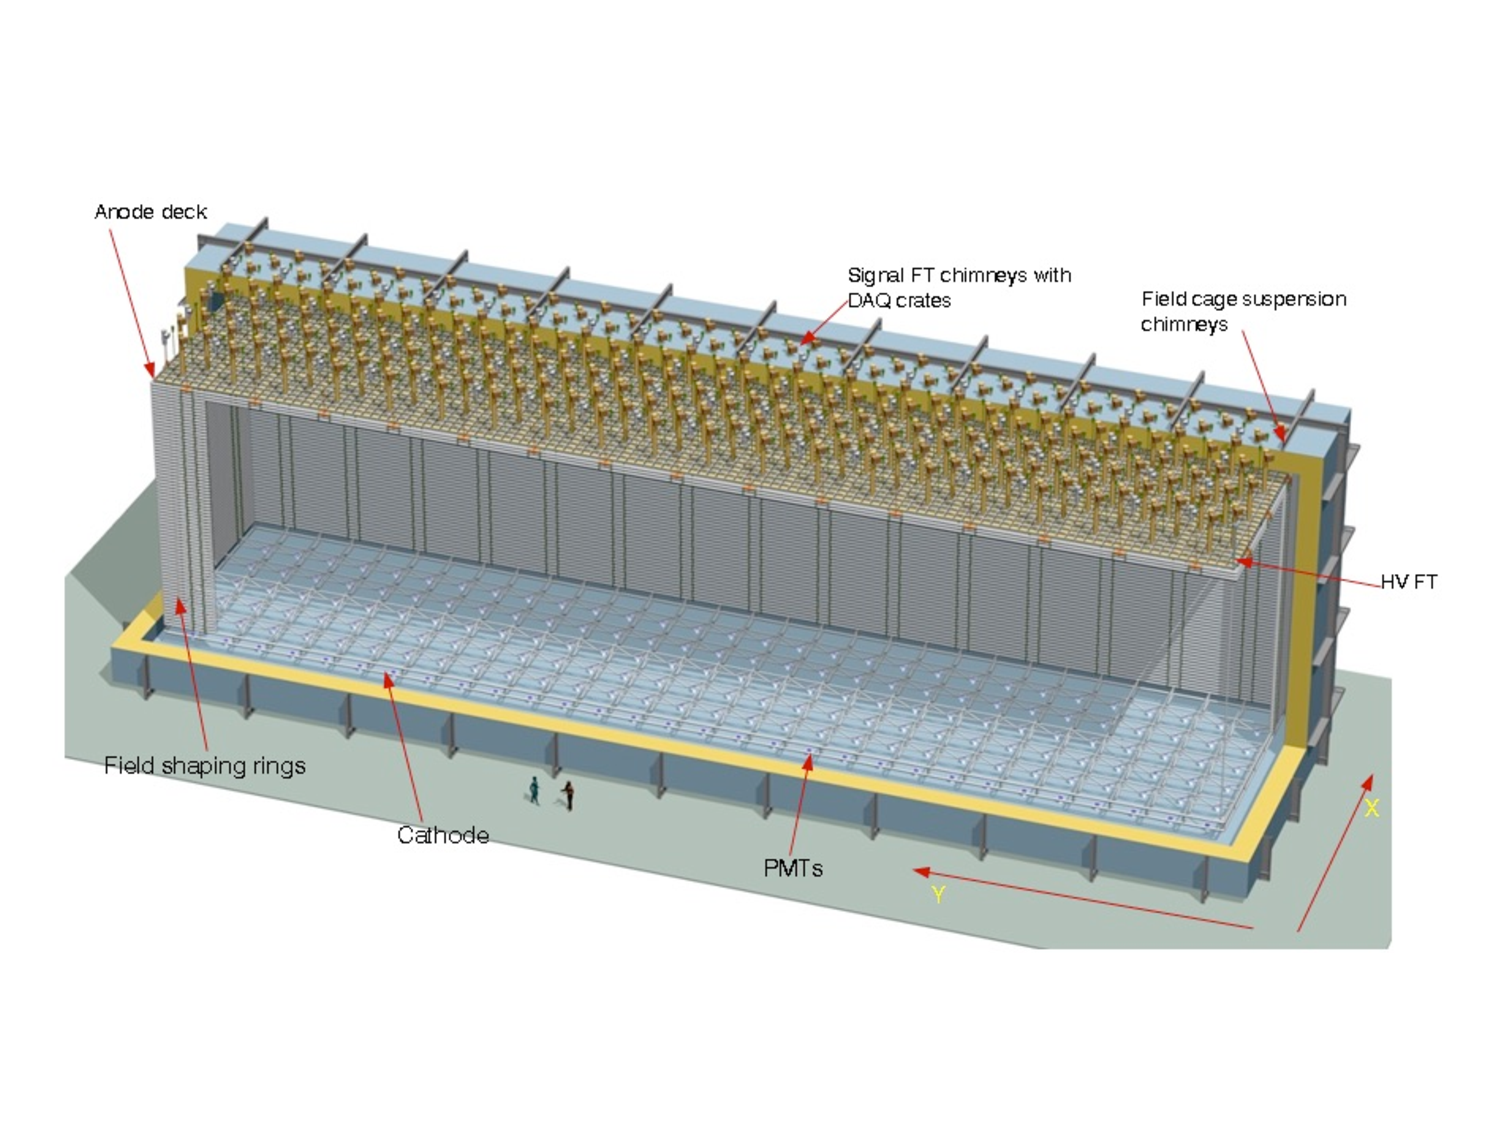
\includegraphics[width=0.95\textwidth]{dppd_3_1}
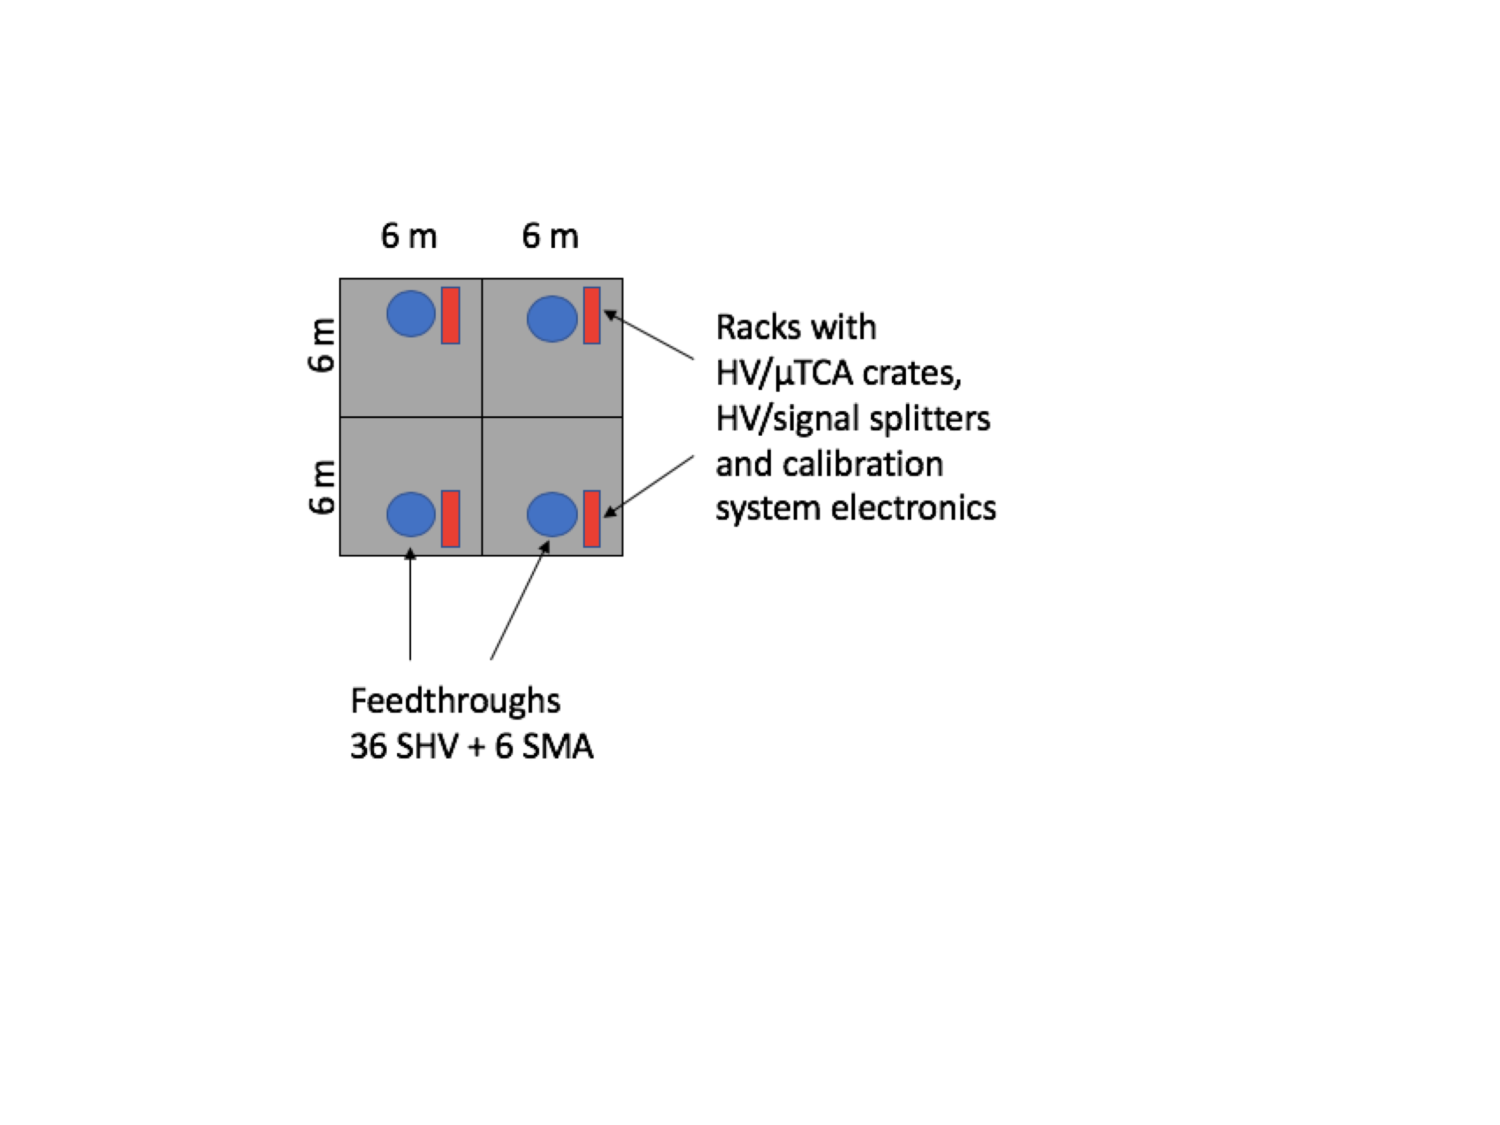
\includegraphics[width=0.55\textwidth]{dppd_1_2}
\end{dunefigure}

The cathode plane, described in Chapter~\ref{ch:dp-hv}, is placed approximately \SI{2}{m} above the bottom of the cryostat. Given the high dielectric constant of the \lar phase, the \dword{pmt} plane is a safe distance from the cathode plane. To protect the \dwords{pmt}, the ground grid is installed and placed at an identical potential as the \dword{pmt} photocathode (\SI{0}{V}).

%%%%%%%%%%%%%%%%%%%%%%%%%%%%%%%%%
\subsection{Operational Modes} %Principles}
\label{sec:dp-pds-oveerview_operation}

The physics program defines the operational modes of the \dual \dword{pds}. Measuring the neutrino oscillation parameters requires recording events upon receiving an external trigger from the beam, while non-beam physics such as \dwords{snb}, proton decay, or other rare events require special trigger conditions that include the \dword{pds}. Another operation mode is the \Dword{pmt} calibration run, which is initiated by the light calibration system with its dedicated hardware trigger.
%
Thus, the operation modes are
\begin{itemize}
\item External trigger: %this is mainly the case of 
A typical case is when the beam generates a hardware trigger (a beam gate);  it also includes software-generated triggers for test data.
\item Non-beam physics trigger: The electronics based on the \dword{pds} signals provides the trigger for, among other events, \dword{snb} and proton decay events;
\item Calibration trigger: The trigger is provided by the light calibration system during \dword{pds} calibrations.
\end{itemize}

The external and non-beam physics triggers run in parallel to ensure that rare events like \dwords{snb} are recorded efficiently. 

%%%%%%%%%%%%%%%%%%%%%%%%%%%%%%%%%
\subsection{Detector Design Specifications}
\label{sec:dp-pds-overview_specs}

The \dual \dword{pds} detector specifications are given in Table~\ref{tab:specs:just:DP-PDS}. The physics-driven rationale for each detector specification, and the means to validate them, are also summarized in the table. Validation of the detector specifications uses data from \dword{pds} prototypes (Section~\ref{sec:dp-pds-prototypes}) and from a full simulation/reconstruction of signal and background optical flashes in the \dpmod (Section~\ref{sec:dp-pds-performance}). 

%\fixme{(from Anne) Here is your requirements table. For SP, we've asked each chapter to include the "top 5" of the FD specs. That may not be appropriate for DP, since those top-level specs (approved by EB) may not exist yet.}

%% This file is generated, any edits may be lost.

\begin{longtable}{p{0.14\textwidth}p{0.13\textwidth}p{0.18\textwidth}p{0.22\textwidth}p{0.20\textwidth}}
\caption{Specifications for DP-PDS \fixmehl{ref \texttt{tab:spec:DP-PDS}}} \\
  \rowcolor{dunesky}
       Label & Description  & Specification \newline (Goal) & Rationale & Validation \\  \colhline

    \\ \rowcolor{dunesky} \newtag{SP-FD-1}{ spec:min-drift-field } & Name: Minimum drift field \\
    Description & The drift field in the TPC shall be greater than 250 V/cm, with a goal of 500 V/cm.   \\  \colhline
    Specification (Goal) &  $>$\,\SI{250}{ V/cm}  ( $>\,\SI{500}{ V/cm}$ ) \\   \colhline
    Rationale &   Lessens impacts of e-Ar recombination, e-lifetime, e-diffusion and space charge.  \\ \colhline
    Validation & ProtoDUNE  \\
   \colhline

   
  \newtag{SP-FD-2}{ spec:system-noise }  & System noise  &  $<\,\SI{1000}\,e^-$ &  Provides $>$5:1 S/N on induction planes for  pattern recognition and two-track separation. &  ProtoDUNE and simulation \\ \colhline
    
    \\ \rowcolor{dunesky} \newtag{SP-FD-3}{ spec:light-yield } & Name: Light yield \\
    Description & The light yield shall be sufficient for measuring event time (and total intensity) of events with visible energy above 200 MeV.  Goal is to make possible a 10\% energy measurement for events with a visible energy of 10 MeV.   \\  \colhline
    Specification (Goal) &  $>\,\SI{0.5}{pe/MeV}$  ( $>\,\SI{5}{pe/MeV}$ ) \\   \colhline
    Rationale &   Rejects nucleon decay backgrounds from cosmogenic events near cathode.  \\ \colhline
    Validation &   \\
   \colhline

   \newtag{SP-FD-4}{ spec:time-resolution-pds }  & Time resolution  &  $<\,\SI{1}{\micro\second}$ \newline ( $<\,\SI{100}{\nano\second}$ ) &  Enables \SI{1}{mm} position resolution for \SI{10}{MeV} SNB candidate events for instantaneous rate $<\,\SI{1}{m^{-3}ms^{-1}}$. &   \\ \colhline
    
    \\ \rowcolor{dunesky} \newtag{SP-FD-5}{ spec:lar-purity } & Name: Liquid argon purity \\
    Description & The LAr purity shall remain lower than 100 ppt (with a goal of < 30 ppt). This corresponds to e- lifetime of 3 (10) ms.   \\  \colhline
    Specification (Goal) &  $<$\,\SI{100}{ppt}  ( $<\,\SI{30}{ppt}$ ) \\   \colhline
    Rationale &   Provides $>$5:1 S/N on induction planes for  pattern recognition and two-track separation.  \\ \colhline
    Validation & Purity monitors and cosmic ray tracks  \\
   \colhline


   
  \newtag{DP-PDS-1}{ spec:dp-light-yield }  & Light yield  &  $>\,\SI{1}{PE/MeV}$ at anode, $>\,\SI{5}{PE/MeV}$ avg over  active vol &  Enable drift position determination of \dword{ndk} candidates. Enable \dword{pds}-based triggering on galactic \dwords{snb}. &  Full sim/reco of \dword{ndk}, \dword{snb} $\nu$ and radiological events. \\ \colhline
    
   \newtag{DP-PDS-2}{ spec:dp-time-resolution }  & Time resolution  &  $<\,\SI{1}{\micro\second}$ \newline ( $<\,\SI{100}{\nano\second}$ ) &  Enables \SI{1}{mm} pos resolution for \SI{10}{MeV} \dwords{snb} candidate events for instantaneous rate $<\,\SI{1}{m^{-3}ms^{-1}}$. &   \\ \colhline
    
   
  \newtag{DP-PDS-3}{ spec:dp-lar-nitrogen-contamination }  & LAr nitrogen contamination  &  $<\,\SI{3}{ppm}$ &  Higher contaminations signifcantly affect the no. of photons that reach the \dword{pmt}. &   \\ \colhline
    
   
  \newtag{DP-PDS-4}{ spec:hit-relative-timing }  & Relative timing accuracy among hits  &  $<\,\SI{100}{ns RMS}$ &  Enable effective clustering of \dword{pmt} signals based on relative hit timing information. &  Full sim/reco of \dword{ndk}, \dword{snb} $\nu$ and radiological events. \\ \colhline
    
   
  \newtag{DP-PDS-5}{ spec:hit-snr }  & Hit signal-to-noise ratio  &  $>\,\num{5}$ &  Efficiently reconstruct single-\phel hits while rate of electronics noise hits remains manageable. &  Single-\phel and baseline noise \dword{rms} measurements in $3\times1\times1$ prototype. \\ \colhline
    
   
  \newtag{DP-PDS-6}{ spec:pmt-dark-rate }  & PMT dark count rate  &  $<\,\SI{100}{kHz}$ &  Avoid effects on clustering algorithm and \dword{pds}-based calorimetry. &  Characterization of \dwords{pmt} at cryo temps prior to installation. \\ \colhline
    
   
  \newtag{DP-PDS-7}{ spec:pds-analog-range }  & Analog range per channel  &  $>\,\SI{100}{PE/(channel\times 6\nano\second)}$ &  Minimize hit saturation for scintillation-based calorimetry over \SI{6}{ns} prompt light period, esp. for beam events. &  Full sim/reco of beam $\nu$ interactions.  \\ \colhline
    


\label{tab:specs:DP-PDS}
\end{longtable}

%\fixme{The next table is just the DP PDS. It doesn't include the two SP FD requirements you selected (3 and 15 I think).}
% This file is generated, any edits may be lost.

\begin{longtable}{p{0.14\textwidth}p{0.13\textwidth}p{0.18\textwidth}p{0.22\textwidth}p{0.20\textwidth}}
\caption{Specifications for DP-PDS \fixmehl{ref \texttt{tab:spec:DP-PDS}}} \\
  \rowcolor{dunesky}
       Label & Description  & Specification \newline (Goal) & Rationale & Validation \\  \colhline

   
  \newtag{DP-PDS-1}{ spec:dp-light-yield }  & Light yield  &  $>\,\SI{1}{PE/MeV}$ at anode, $>\,\SI{5}{PE/MeV}$ avg over  active vol &  Enable drift position determination of \dword{ndk} candidates. Enable \dword{pds}-based triggering on galactic \dwords{snb}. &  Full sim/reco of \dword{ndk}, \dword{snb} $\nu$ and radiological events. \\ \colhline
     % 1
   \newtag{DP-PDS-2}{ spec:dp-time-resolution }  & Time resolution  &  $<\,\SI{1}{\micro\second}$ \newline ( $<\,\SI{100}{\nano\second}$ ) &  Enables \SI{1}{mm} pos resolution for \SI{10}{MeV} \dwords{snb} candidate events for instantaneous rate $<\,\SI{1}{m^{-3}ms^{-1}}$. &   \\ \colhline
     % 2
   
  \newtag{DP-PDS-3}{ spec:dp-lar-nitrogen-contamination }  & LAr nitrogen contamination  &  $<\,\SI{3}{ppm}$ &  Higher contaminations signifcantly affect the no. of photons that reach the \dword{pmt}. &   \\ \colhline
     % 3
   
  \newtag{DP-PDS-4}{ spec:hit-relative-timing }  & Relative timing accuracy among hits  &  $<\,\SI{100}{ns RMS}$ &  Enable effective clustering of \dword{pmt} signals based on relative hit timing information. &  Full sim/reco of \dword{ndk}, \dword{snb} $\nu$ and radiological events. \\ \colhline
     % 4
   
  \newtag{DP-PDS-5}{ spec:hit-snr }  & Hit signal-to-noise ratio  &  $>\,\num{5}$ &  Efficiently reconstruct single-\phel hits while rate of electronics noise hits remains manageable. &  Single-\phel and baseline noise \dword{rms} measurements in $3\times1\times1$ prototype. \\ \colhline
     % 5
   
  \newtag{DP-PDS-6}{ spec:pmt-dark-rate }  & PMT dark count rate  &  $<\,\SI{100}{kHz}$ &  Avoid effects on clustering algorithm and \dword{pds}-based calorimetry. &  Characterization of \dwords{pmt} at cryo temps prior to installation. \\ \colhline
     % 6
   
  \newtag{DP-PDS-7}{ spec:pds-analog-range }  & Analog range per channel  &  $>\,\SI{100}{PE/(channel\times 6\nano\second)}$ &  Minimize hit saturation for scintillation-based calorimetry over \SI{6}{ns} prompt light period, esp. for beam events. &  Full sim/reco of beam $\nu$ interactions.  \\ \colhline
     % 7


\label{tab:specs:just:DP-PDS}
\end{longtable}

\section{Photosensor System}
\label{sec:fddp-pds-photosensor}




\section{Mechanics}
\label{sec:dp-pds-mechanics}

\subsection{\dshort{pmt} Support Structure}
\label{subsec:dp-pds-mechanics-pmtsupport}

A uniform array of \dpnumpmtch cryogenic Hamamatsu R5912-MOD20 \dwords{pmt}, below the transparent cathode structure, will be fixed on the membrane floor in the areas between the membrane corrugations. The arrangement of the \dwords{pmt} accommodates the cryogenic piping on the membrane floor, and other elements installed in this area.

The mechanics for the attachment of the \dwords{pmt} were carefully studied. The \dword{pmt} buoyancy must be counteracted while avoiding stress to the \dword{pmt} glass due to differentials in the thermal contraction between the support and the \dword{pmt} itself. The attachment is done via a stainless steel support base point-glued to the membrane via four adhesive injection holes. The weight of the support and \dword{pmt} (approximately \SI{7}{\kg}) exceeds the buoyancy force of the system. Given the large standing surface of the stainless steel plate, these supports also ensure stability against possible lateral forces acting on the \dwords{pmt} due to the liquid flow. Figure \ref{fig:dppd_3_2} shows the \dword{pmt} with its support base attached to the bottom of the \dword{pddp} cryostat.

%\begin{dunefigure}[Cryogenic Hamamatsu R5912-MOD20 \dword{pmt} %fixed on the membrane floor.]{fig:dppd_3_2}
%{Cryogenic Hamamatsu R5912-MOD20 \dword{pmt} fixed on the membrane floor, with the optical fiber of the calibration system.}
%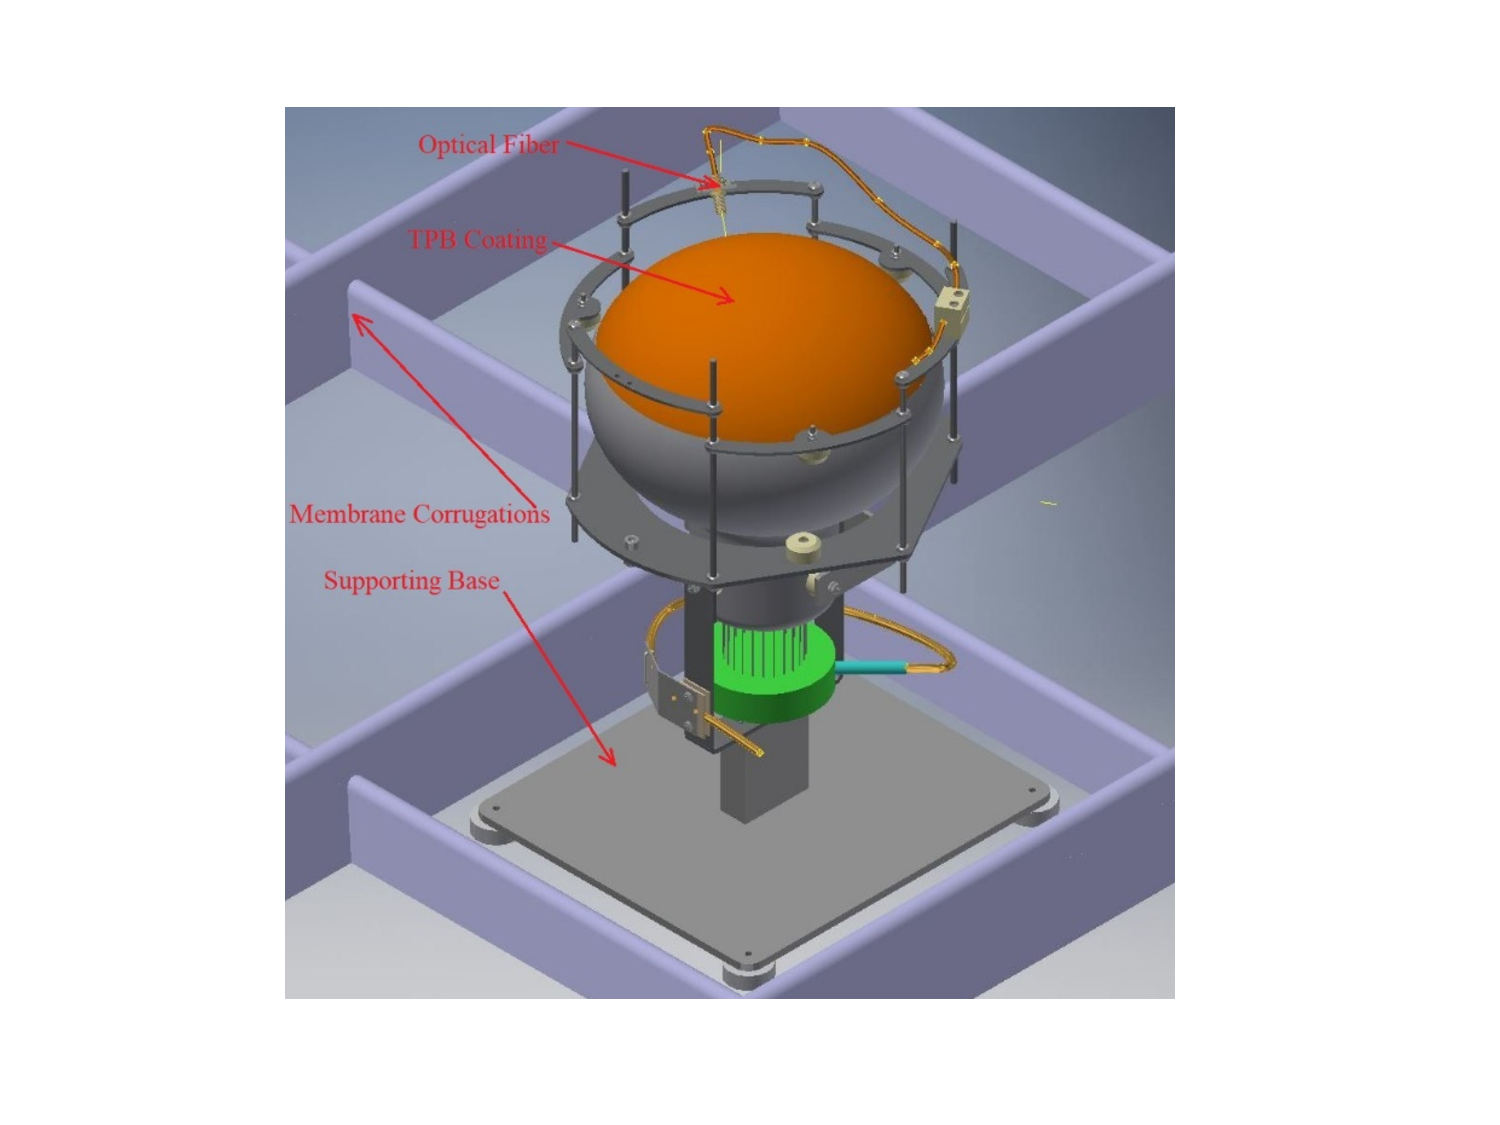
\includegraphics[width=0.42\textwidth]{dppd_3_2}
%\end{dunefigure}

\begin{dunefigure}[Picture of the Hamamatsu R5912-MOD20 \dword{pmt} fixed on the membrane floor of \dword{pddp}.]{fig:dppd_3_2}
{Picture of the cryogenic Hamamatsu R5912-MOD20 \dword{pmt} fixed on the membrane floor of \dword{pddp}. The optical fiber of the calibration system is also visible.}
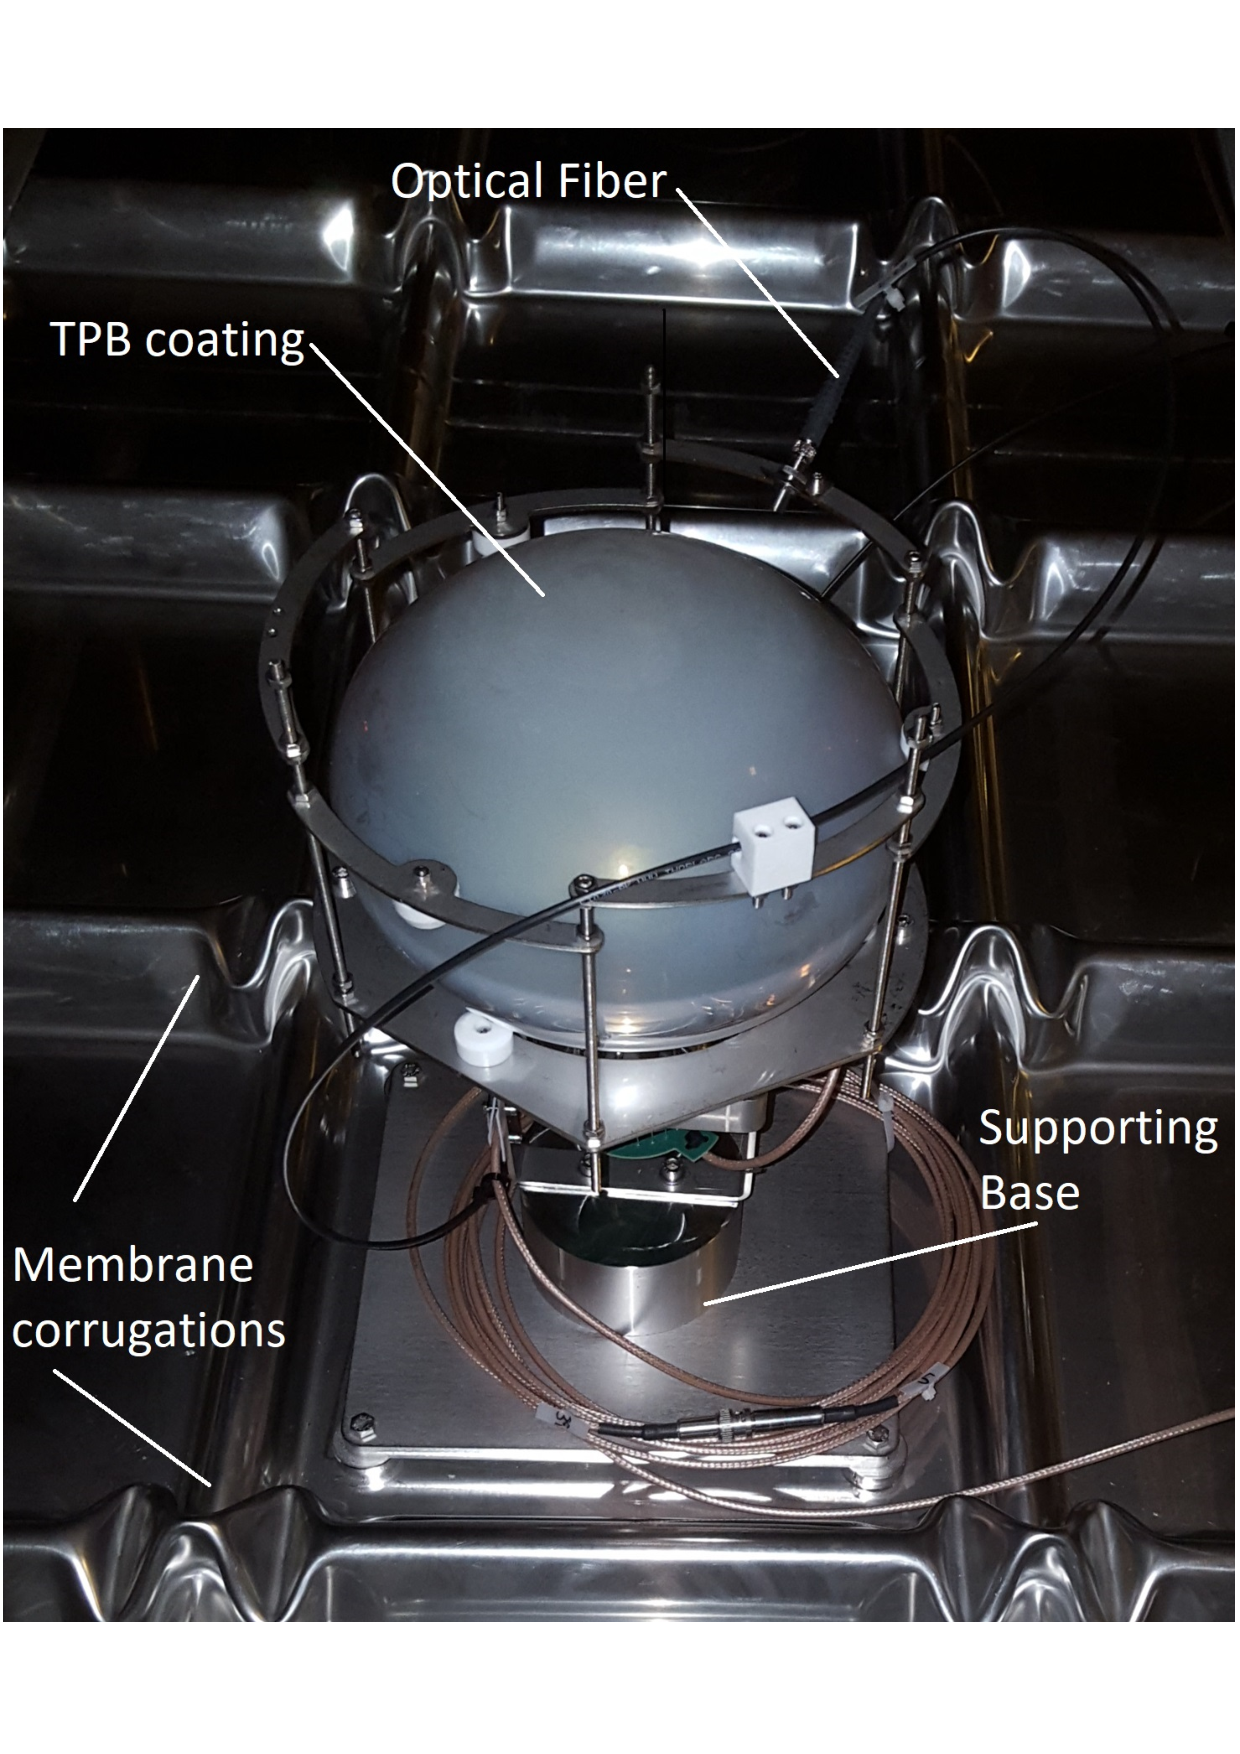
\includegraphics[width=0.42\textwidth]{dppd_3_n2}
\end{dunefigure}

%\fixme{Update Fig.~\ref{fig:dppd_3_2} of PMT support structure.}

%The \dword{hv} and \dual \dword{pds} consortia is studying an alternative to the table-like assembly of the ground grid: the concept of individual ground grids for each \dword{pmt}. In this option, the grids would be mechanically attached to the support structure. This will increase the acceptance of the \dwords{pmt} at larger angles.

The support frame structure mainly comprises \num{304}L stainless steel with some small Teflon (PTFE) pieces assembled by A4 stainless steel screws that minimize the mass while securing the \dword{pmt} support to the cryostat membrane. The design %was done taking 
takes into account the shrinking of the different materials during the cooling process to avoid breaking the \dword{pmt} glass.
Over-pressure tests were carried out for \dword{pddp}, and further tests ensure correct performance under pressure. An individual \dword{pmt} mount has been designed and tested in the  \dword{wa105} prototype~\cite{Zambelli:2017dkg}, and the same design is used for \dword{pddp}.

Installation of an individual ground grids mechanically attached to the \dword{pmt} support structures is also under consideration by the \dword{hv} and \dual \dword{pds} consortia (See Appendix~\ref{sec:dp-pds-appendix-grid}).

%%%%%%%%%%%%%%%%%%%%%%%%%%%%%%%%%%%%%%%%%%%%%%%%%%%%%%%%%%%%%%%%%%%

\subsection{Reflector/\dshort{wls} Panel Assemblies}
\label{subsec:dp-pds-mechanics-reflectors}

The reflector/\dword{wls} panels that will be mounted on the inner surface of the \dword{fc} will be \SI{1}{\mm} thick \SI{93}{\cm} $\times$ \SI{93}{\cm} G10/FR4 plates, with the central \SI{91}{\cm} (H) $\times$ \SI{93}{\cm} (W) area laminated with reflective foil, which is coated with \dword{tpb} (see Fig.~\ref{fig:dppd_reflective_panel}). The panels will be supported by G10/FR4 support bars. Six horizontal bars of \SI{199}{\cm} (three at the front and three at the back), six vertical bars of \SI{186}{\cm} (all at the back) and four reflector/\dword{wls} panels will form a unit reflector/\dword{wls} panel assembly to be mounted on the \dword{fc}. The panels will be sandwiched between the horizontal support bars along the non-laminated edges. Six vertical bars will be placed on the side of the panels without the reflective coating, aligning the holes. The structure will then be assembled by placing \num{24} screws.

The horizontal support bars will be attached to the FRP I-beams of the \dword{fc}, which are spaced \SI{2}{\m} apart, by stainless steel screws. One end of the bar will be tightly screwed, while the other loosely to allow motion due to differential thermal contractions. Figure \ref{fig:dppd_reflective_panel_support} shows sketches of the horizontal support bars with one of the two screw holes elongated to allow the support bar movement on the mounting screw.

\begin{dunefigure}[Sketches of the reflector/\dword{wls} panel assembly horizontal support bars.]{fig:dppd_reflective_panel_support}
{Sketches of the reflector/\dword{wls} panel assembly horizontal support bars (not to scale). (a) The top and bottom bars, (b) the middle bar, (c) the extended top and bottom bars to be mounted on the end submodules of the \dword{fc} super-modules, and (d) the special extended top and bottom bars to be mounted on the end submodules of the corner \dword{fc} side wall super-modules.}
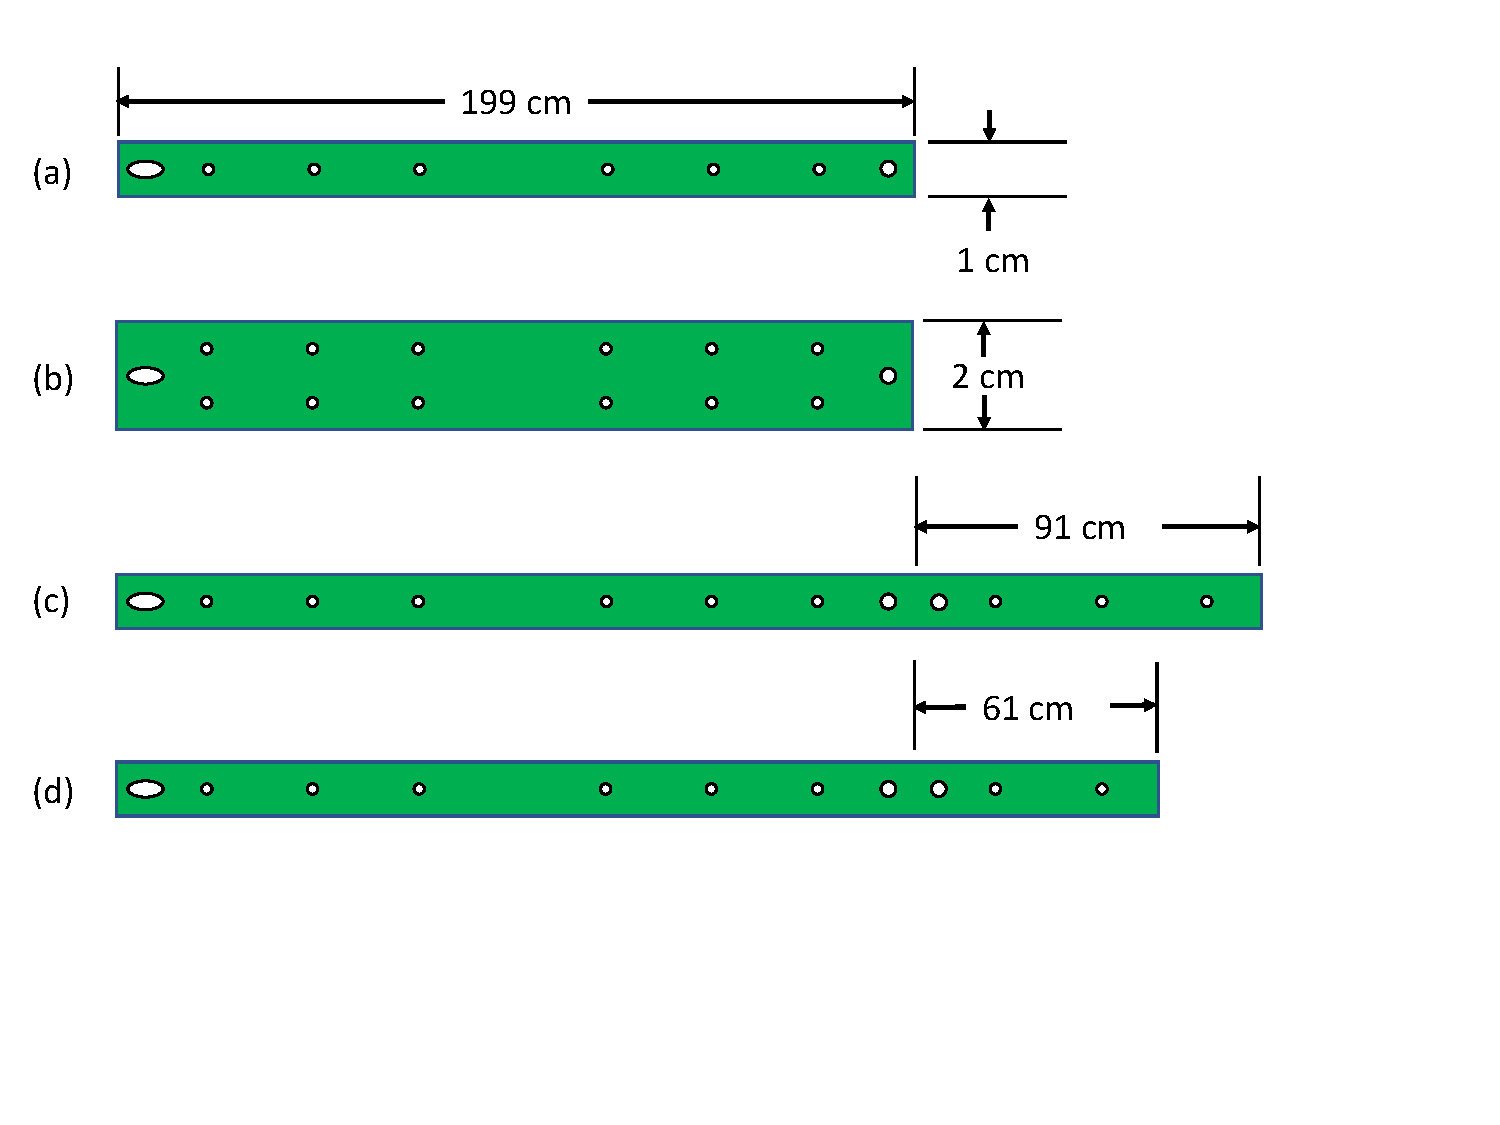
\includegraphics[width=0.65\textwidth]{dppd_reflective_panel_support}
\end{dunefigure}

The reflector/\dword{wls} panel assemblies at the inter-super-module areas will have extended structures: \SI{260}{\cm} (W) $\times$ \SI{186}{\cm} (H) for the corner side wall \dword{fc} sub-modules to accommodate the \num{2.4} degree tilt of the end walls, and \SI{290}{\cm} (W) $\times$ \SI{186}{\cm} (H) for all other \dword{fc} sub-modules at the intersection of two \dword{fc} super-modules. The extended assemblies will house \num{6} reflector/\dword{wls} panels, two of them in an extended part which is not supported at the end. Figure \ref{fig:dppd_reflective_panel_support} (c) shows the sketch of the support bar to be installed at the end submodules of the \dword{fc} super-modules except the end submodules of the corner \dword{fc} side wall super-modules of which the corresponding horizontal support bar is shown in Fig.~\ref{fig:dppd_reflective_panel_support} (d). The special extended assemblies to be installed at the end submodules of the corner side wall super-modules will be \SI{30}{\cm} shorter than the regular extended assemblies to accommodate the approximately \SI{25}{\cm} approach of the end walls at middle drift distance (\SI{6}{\m}).

Figure \ref{fig:dppd_reflective_panel_onFC} shows inside (left) and outside (right) sketches of a unit reflector/\dword{wls} assembly. The blue bars are the I-beams of the \dword{fc}, the dark green bars are the horizontal and vertical support bars of the reflector/\dword{wls} panel assembly. The grey surfaces are the \dword{tpb} coatings on the panels. The vertical and horizontal gaps between the reflector/\dword{wls} panels allow liquid flow. 

\begin{dunefigure}[Sketches of the inside and outside views of a partial \dword{fc} submodule with a reflector/\dword{wls} panel assembly.]{fig:dppd_reflective_panel_onFC}
{Sketches of the inside with the reflective/\dword{wls} coating (left) and outside without the reflective/\dword{wls} coating (right) views of a partial \dword{fc} submodule with a reflector/\dword{wls} panel assembly. The blue bars are the FRP I-beams of the \dword{fc}. The dark green bars are the horizontal and vertical support bars. The grey surfaces are the \dword{tpb} coatings on the panels.}
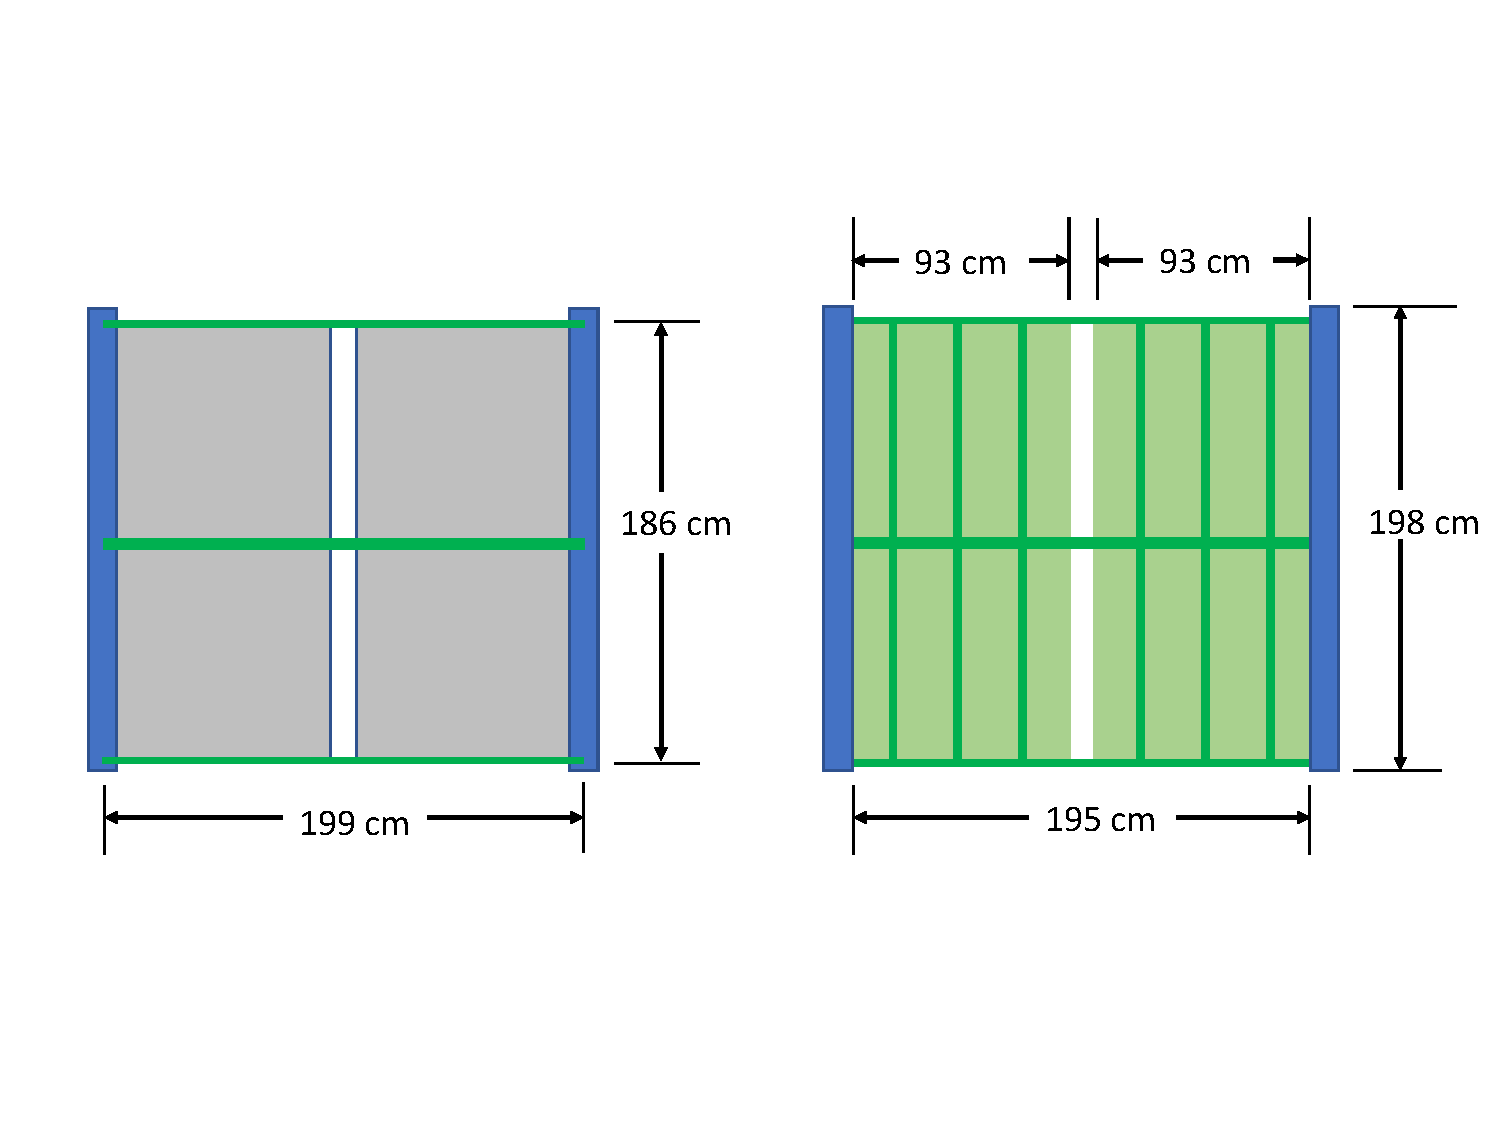
\includegraphics[width=0.8\textwidth]{dppd_reflective_panel_onFC}
\end{dunefigure}
\section{Readout Electronics}
\label{sec:fddp-pds-electronics}



\section{Calibration System}
\label{sec:dp-pds-calibration}

A photon calibration system is required in the DP module to calibrate the \dwords{pmt} installed in the \dword{lar} volume. The goal is to determine the \dword{pmt} gain and monitor the stability of the \dword{pmt} response. One of the main goals of the \dword{pds} is to provide a trigger for non-beam physics. The trigger is based on the amplitude of \dword{pmt} signals. The amplitudes of the \dword{pmt} signals are summed for groups of certain \dwords{pmt} and/or for all \dwords{pmt} and then, these input signals are discriminated according to the trigger logic. An equalized \dword{pmt} response allows using the same threshold definition for all \dword{pmt} groups, simplifying the determination of trigger efficiency. In addition to measuring the \dword{pmt} gain, the calibration system is also designed to monitor the stability of the \dword{pmt} response. % and its quantum efficiency. 
In addition to the necessary \dword{pmt} characterization at cryogenic temperature before installation~\cite{Belver:2018erf}, and based on past experience with \dword{wa105} detector operations~\cite{Aimard:2018yxp}, we conclude that a light calibration system is needed during experiment data taking.

%%%%%%%%%%%%%%%%%%%%%%%%%%%%%%%%%%%%%%%%%%%%%%%%%%%%%%%%%%%%%%%%%%%%

\subsection{Calibration System Design}

An \dword{led}-driven fiber calibration system~\cite{Cuesta:2017nrs,Conrad:2015xta,Caccianiga:2003fm,ADAMSON2002325,Belver:2019lqm} is designed so a configurable amount of light reaches each \dword{pmt}. The calibration light is provided by a blue \dword{led} of \SI{465}{\nm} using a Kapustinsky~\cite{KAPUSTINSKY1985612} circuit as \dword{led} driver and transmitted by a fiber system ending with an optical fiber installed at each \dword{pmt} (see Figure~\ref{dppd-6-LCS}). Twenty groups of six \dwords{led} placed in a hexagonal geometry and a reference sensor check the performance of the \dword{led} in the center of each group. The direct light goes to the fiber, and the stray light to the \dword{sipm} used as reference sensor. Each \dword{led} is connected to an external fiber going to one feedthrough. Then, fibers are connected inside the cryostat, and each fiber is attached to a 1-to-7 fiber bundle, so that one fiber is finally installed pointing at each \dword{pmt}. The \dwords{pmt} are oriented with the first dynode perpendicular to the Earth magnetic field and the fiber parallel to the first dynode to have a similar gain to the one obtained with diffuse light. The components placed outside the cryostat at room temperature form the \textit{external system}, and the ones installed inside it at cryogenic temperature form the \textit{inner system}. 

%############################################
%\begin{figure}[ht]
%\bigskip
%\centering
% \includegraphics[height=0.6\textwidth]{graphics/LCSdiagram_DUNE.pdf}
%\caption{Sketch of the \dword{dune} \dword{fd} \dfirst{pds} light calibration system. The external system at room temperature is shown in blue and the inner system at cryogenic temperature in black.}
%\label{dppd-6-LCS}
%\end{figure}

\begin{dunefigure}[Sketch of the \dword{dune} \dword{fd} \dword{pds} light calibration system.]{dppd-6-LCS}
{Sketch of the \dword{dune} \dword{fd} \dword{pds} light calibration system. The external system at room temperature is shown in blue and the inner system at cryogenic temperature in black.}
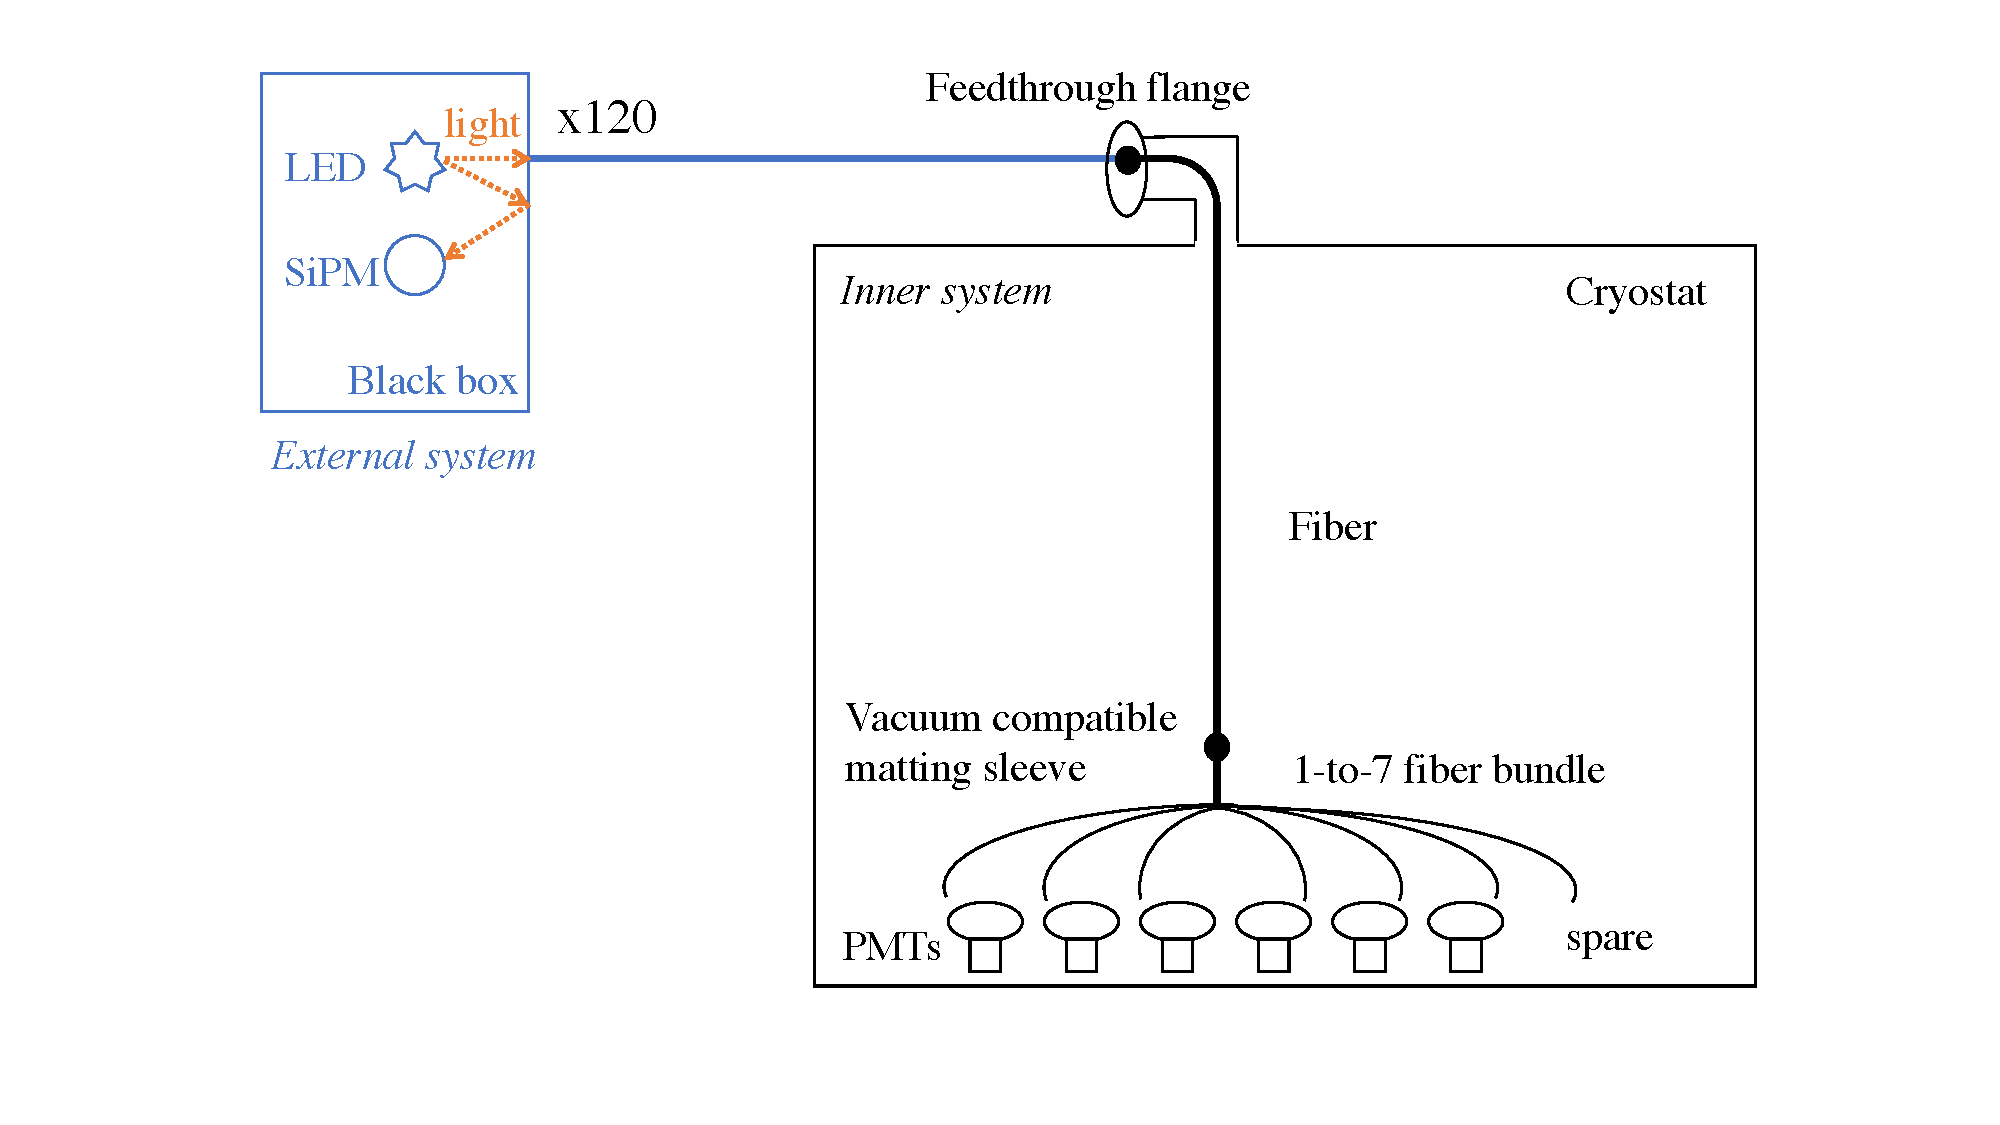
\includegraphics[width=0.7\textwidth]{dppd_LCSdiagram_DUNE}
\end{dunefigure}

%############################################

%%External system
The design of the external components is driven by the need for a cost-effective system. An additional requirement is that a reference light sensor monitors the amount of the injected light. The light is injected in form of several \si{\ns} long pulses provided by a Kapustinsky circuit. The set up consists of a commercial black box in which a light guide structure is mounted. There are \num{20} structures, and each has six arms and a central part, as shown in Figure~\ref{fig_source}. On each of the six arms, an electronics board containing a Kapustinsky circuit is mounted. The \dword{led}, NSPB300B from Nichia Corp.\footnote{www.nichia.com}, with a peak wavelength of \SI{465}{nm} is placed  on the PCB in front of an optical SMA to SMA feedthrough. On the other side of each feedthrough, an optical fiber, FG105LCA-CUSTOM-MUC from Thorlabs\footnote{www.thorlabs.com}, is connected. The fiber transports the light to one of the \num{120} feedthroughs in the instrumentation flange on top of the cryostat. While a large fraction of the LED light is emitted forward, a small fraction, the stray light, is emitted under a large angle and reaches by reflection to the central region of the light guide structure where it is detected by a \dword{sipm}, MicroFJ-30035-TSV-TA from SensL\footnote{www.sensl.com}.


%############################################
%\begin{figure}[h!]
%\centering
%\includegraphics[width=0.25\textwidth]{graphics/LightGuide.jpg}\label{fig:lightguide}
%\includegraphics[width=0.55\textwidth]{graphics/Stray.png}\label{fig:stray}
%\caption{(Left) Picture of the light guide structure during the development phase. The six arms are visible, and on one of them a prototype \dword{led} driver is mounted. (Right) Schematics of the light way from the \dword{led} to the reference sensor.}
%\label{fig_source}
%\end{figure}

\begin{dunefigure}[Picture of the light guide structure during the development phase and the schematics of the light way from the \dword{led} to the reference sensor.]{fig_source}
{(Left) Picture of the light guide structure during the development phase. The six arms are visible, and on one of them a prototype \dword{led} driver is mounted. (Right) Schematics of the light way from the \dword{led} to the reference sensor.}
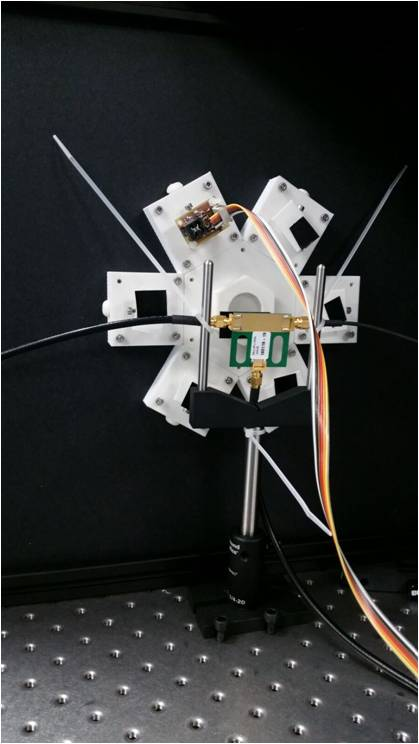
\includegraphics[width=0.25\textwidth]{dppd_LightGuide.jpg}
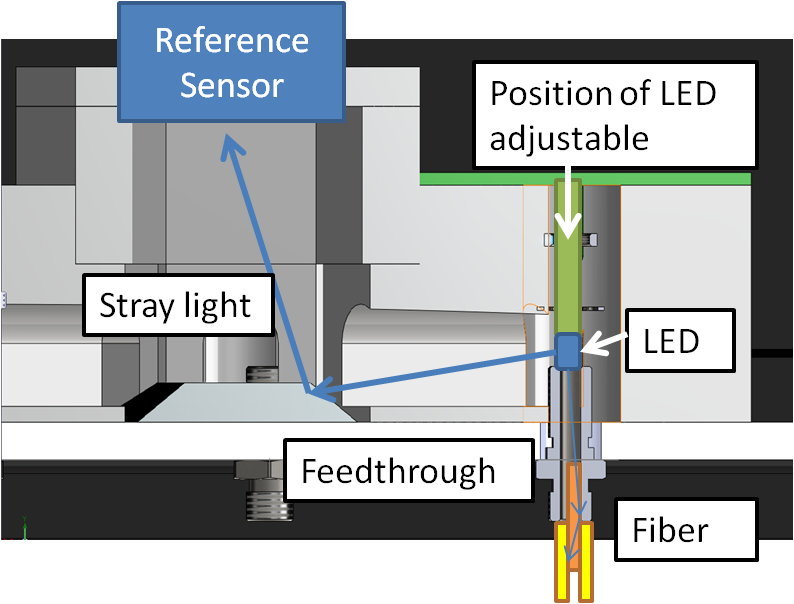
\includegraphics[width=0.6\textwidth]{dppd_Stray.png}
\end{dunefigure}




%############################################

%%Inner system
The inner system is designed to minimize light losses at cryogenic temperatures. The external fibers are connected to 120 female optical feedthroughs from Allectra\footnote{www.allectra.com} installed at \num{20} flanges. Inside the cryostat, a single long fiber, FT800UMT from Thorlabs, goes down from each optical feedthrough routed along the walls of the cryostat to the bottom of the cryostat where a \num{1}-to-\num{7} fiber bundle, comprising FT200UMT fibers from Thorlabs, is connected to each long fiber. A total of \num{720} of these fibers are guided to the \dwords{pmt} at the bottom of the detector. The end of the fiber is fixed at the \dword{pmt} support structure pointing the photocathode. The fibers and bundles are \num{0.39}\,NA TECS$^\text{TM}$ hard-clad, multimode, step-index fibers with high OH (hydroxyl) content to increase the light transmission at low wavelengths. To optimize the light transmission of the fiber-bundle connection, the inner fibers have a diameter of \SI{800}{\um}, big enough to distribute uniformly the light at the bundle entrance, total diameter \SI{700}{\um}. From the mechanical point of view, the described approach of bundles attached to fibers is safer than connecting  the bundles directly to the feedthroughs. To have good homogeneity of the light at the fiber-bundle connections, SMA connectors are chosen. Vacuum compatible SMA to SMA mating sleeves are required to avoid \dword{lar} freezing inside the connector, which would reduce light transmission.

Alternatives to the calibration system baseline design described here are also being considered. See Appendix~\ref{sec:dp-pds-appendix-calibration}. 

%\fixme{Alternatives to illuminate many \dwords{pmt} at once with fibers on top of field cage being investigated for \dword{pddp}. If we end up installing such an alternative design in \dword{pddp}, we should adapt text here.}

%Alternatives to this design will be pursued with R\&D measurements in order to make  it  more  effective,  reduce  the  cost and  mitigate  issues  related  to  the  scaling. These alternatives include reducing the amount of fibers, studying other options for the reference sensor, and increasing the input light if necessary. To reduce the number of fibers, light diffusers can be used, so that one fiber can illuminate at least 4 PMTs. For instance, a diffuser could be placed at the ground grid.

%%Validation measurements
%In order to validate the design, the most important result comes from the ProtoDUNE-DP performance. In any case, since the fibers to be used in DUNE FD will be longer, dedicated calculations and measurements to confirm that sufficient light reaches the PMTs will be performed. Also, alternative designs, will be validated in different laboratories.  The possibility of using a diffuser can be tested in a vessel. The light source will also be validated by studying the different options in the lab. All these measurements will be performed at room temperature and in liquid nitrogen to test the behavior at cryogenic temperatures. Once the design is fixed, basic characterization measurements will be performed on the fibers upon receiving them from the manufacturer. Those measurements will consist of providing light with a known source and measuring the output with a power meter. Measurements at cryogenic temperatures may not be needed at this point.

%Finally, during the photon calibration system installation, each fiber and source will be re-tested to check that the expected light is arriving to each PMT using a photodiode. A dedicated procedure will be designed with this purpose, similar to the one used in ProtoDUNE-DP.

\section{Photon Detector Simulation}
\label{sec:dp-pds-simulation}

A detailed simulation of the \dshort{pds} response is essential both to compare with data from \dshort{pds} prototypes (see Section~\ref{sec:dp-pds-prototypes}) and to validate the \dword{fd} baseline design for its projected performance (see Section~\ref{sec:dp-pds-performance}).

%%%%%%%%%%%%%%%%%%%%%%%%%%%%%%%%%%%%%%%%%%%%%%%%%%%%%%%%%%%%%%%%%%%

\subsection{Simulation Framework And Assumptions}
\label{subsec:dp-pds-simulation_assumptions}

The simulation of the \dword{pds} response is integrated in \dword{larsoft}, the liquid argon software toolkit used by the \dune Collaboration for simulation and reconstruction. The simulation is divided in three steps: light generation, light propagation, and light detection.

For a \dword{mip}, an energy of about \SI{2}{\MeV/\cm} is deposited in \dword{lar}. Through decays of excited argon states and ion recombination, about \num{40000} scintillation photons are emitted per \si{\MeV} deposited at null drift field. At the nominal drift field of \SI{500}{\V/\cm}, this amount reduces down to about \num{24000} photons per \si{\MeV} as the recombination process weakens. This signal, known as S1 (see Section~\ref{sec:dp-pds-overview}), is common to the single and dual phase technologies.

In the gas layer of the dual phase design, the electrons are amplified through Townsend avalanche in the \dword{lem} holes and lead to an electroluminescence signal called S2 (see Section~\ref{sec:dp-pds-overview}). The electroluminescence gain, $G_{EL}$, i.e., the number of photons produced per electron crossing the liquid-gas interface, depends on the voltages applied to the \dword{lem}. In our simulations, we typically assume a gain of \SI{300}{photons per extracted electron}. The S1 and S2 signals have similar characteristics for wavelength and time constants. 

Because of different mechanisms during photon propagation (Rayleigh scattering, absorption by impurities in the \lar or by elements constituting the detector), only \num{1e-3} fraction of the photons produced in the \lar active volume reaches the \dword{pmt} photo-cathodes. The direct simulation of the large number of photons generated for each track crossing the active volume would require a considerable amount of CPU power and time. Profiting from the fact that the photon emission is isotropic and the detector is uniform and symmetric, it was decided to generate the photon propagation in the detector in a dedicated Geant4 simulation only once and then to store the results in a photon library.

The active volume is divided into voxels, and a large number of photons are isotropically and uniformly generated in every voxel. The number of photons collected by each \dword{pmt} and the propagation time are stored and later parametrized. For long voxel-\dword{pmt} distances (typically larger than \SI{1}{\m}), a landau function is well suited to reproduce the time distribution. The detection probability, called visibility, the landau parameters (most probable value, $\sigma$) and the minimal time needed by the photon to reach the \dword{pmt} are stored in a photon library for all voxel-\dword{pmt} combinations. When a track is generated in the standard \dual \dword{larsoft} simulation toolkit, for each step of the track, the light map is looked up to assign the number of photons to be collected at each \dword{pmt} and the arrival time distribution due to the propagation. 

To generate photon libraries, a comprehensive modelling of the geometry for the \dword{wa105}, \dword{pddp}, and \dword{dp} \dword{fd} detectors are implemented in \dword{gdml} files. The \dword{gdml} files include the main elements relevant for light propagation, such as the cathode, the \dword{fc}, the \dwords{lem}, and the ground grid. Most detector elements are assumed to be fully absorptive. Thus, when photons reach any of these surfaces, they are removed from the simulation. One exception is \dword{wls} reflector foil surfaces, which are assumed to have \SI{100}{\%} \dshort{wls} efficiency for \SI{127}{\nm} \dshort{lar} light and 93\% reflectivity for \SI{430}{\nm} light re-emitted by the wavelength shifter material. To quantify the effect of the \dshort{wls} reflector foils for the \dword{dp} \dword{fd} module, three geometries have been tested: no foils, foils entirely covering all four \dword{fc} vertical walls (full foils, in the following), and foils covering only the upper half of the \dword{fc} (half foils, in the following). For the \dword{pds} prototypes, no foil geometries have been simulated.

As far as \dword{lar} optical properties are concerned, the simulations assume a \SI{61}{\cm} Rayleigh scattering length for \SI{127}{\nm} light, no Rayleigh scattering for visible light, and a \SI{20}{\m} absorption length for all wavelengths. The response of the \dword{pmt} is simulated assuming an effective quantum efficiency of \num{0.12} for \SI{127}{\nm} light. This value includes the \dword{tpb} response of the coated photo-cathode \cite{Bonesini:2018ubd}. For visible light emitted by \dword{wls} foils, the \dword{pmt} quantum efficiency is taken to be \num{0.20}. A dark count rate of \SI{1.7}{\kilo\hertz} at cryogenic temperature is assumed, as obtained during \dword{pddp} \dword{pmt} calibration \cite{Belver:2018erf}. A linear response of the \dword{pmt} is assumed, multiplying the number of photons reaching the photo-cathode with the single photo-electron response measured in the laboratory for a gain of \num{1e7}. In this case, the single-PE response has a time width of \SI{6}{\nano\s}, and an amplitude of \SI{15}{mV}. The digitization of the waveform is simulated considering a sampling rate of \SI{250}{MHz}\footnote{This is the sampling frequency used in the \dshort{wa105} readout, but slower frequencies of \SI{65}{MHz} or \SI{2.5}{MHz} are being considered for the \dword{dp} \dword{pds}.}, a resolution of \SI{0.5}{mV/ADC}, and an electronics noise of \SI{0.8}{ADC counts \dword{rms}} as measured in \dshort{wa105}, see Section~\ref{sec:dp-pds-prototypes}. Therefore, based on \dshort{wa105} measurements, the \dword{spe} to baseline noise \dword{rms} ratio assumed in the simulations exceeds \num{30}.

%%%%%%%%%%%%%%%%%%%%%%%%%%%%%%%%%%%%%%%%%%%%%%%%%%%%%%%%%%%%%%%%%%%

\subsection{Expected Light Yields}
\label{subsec:dp-pds-simulation_yields}

Table~\ref{tab:dp-pds-light-yields} gives the detected light yields expected in the \dune \dword{fd} geometry, for the three different \dword{wls} reflector foil geometries mentioned above. The yield is computed by averaging over all \lar voxels contained in the \dword{tpc} active volume. A voxel size of \SI{1}{\m^3} is considered in \dword{dp} \dshort{fd} simulations. The average yield is \num{5.4}, \num{8.0} and \SI{12.2}{PEs/MeV} for the no foils, half foils and full foils geometries, respectively. The higher yield for the foil geometries is partly due to the higher number of photons reaching the \dword{pmt} photo-cathodes, and partly due to the higher \dword{pmt} quantum efficiency for visible light. As shown in Table~\ref{tab:dp-pds-light-yields}, a 11.3\% (33.8\%) fraction of photons reaching the \dwords{pmt} is \dword{wls} visible light, in the half foils (full foils) geometry.

\begin{dunetable}
[Average light yields in the \dune \dword{fd} geometry.]
{crrr}
{tab:dp-pds-light-yields}
{Average light yields in the \dune \dword{fd} geometry for different \dword{wls} reflector foil configurations. The total incident light yields and the fractions of incident \dword{wls} light at the \dword{pmt} photo-cathodes, as well as the total detected light yields, are given.}
%\rowcolor{dunesky} 
Configuration & Incident light yield & Fraction of incident & Detected light yield \\
\rowcolor{dunesky} 
 & (photons/\si{MeV}) & \dword{wls} light (\%) & (PEs/\si{MeV}) \\ 
%\hline
No Foils   &  45 &  0.0 &  5.4 \\
Half Foils &  62 & 11.3 &  8.0 \\
Full Foils &  83 & 33.8 & 12.2 \\ 
%\hline
\end{dunetable}

\begin{dunefigure}[Expected 1D light yields in the full \dword{dp} \dshort{fd} cryostat.]{fig:dppd_fd_light_yield_comparisons}
{Expected light yield in the full \dword{dp} \dshort{fd} cryostat. The yield units are number of photo-electrons per \si{\MeV} of deposited energy. The 1D yields are shown as a function of the drift (transverse) direction in the left (right) panel, averaging over the other two spatial coordinates (not shown). The three histograms correspond to three different geometries: no \dword{wls} reflector foils, foils fully covering \dword{fc}, foils covering upper \dword{fc} half.}
\raisebox{0.1cm}{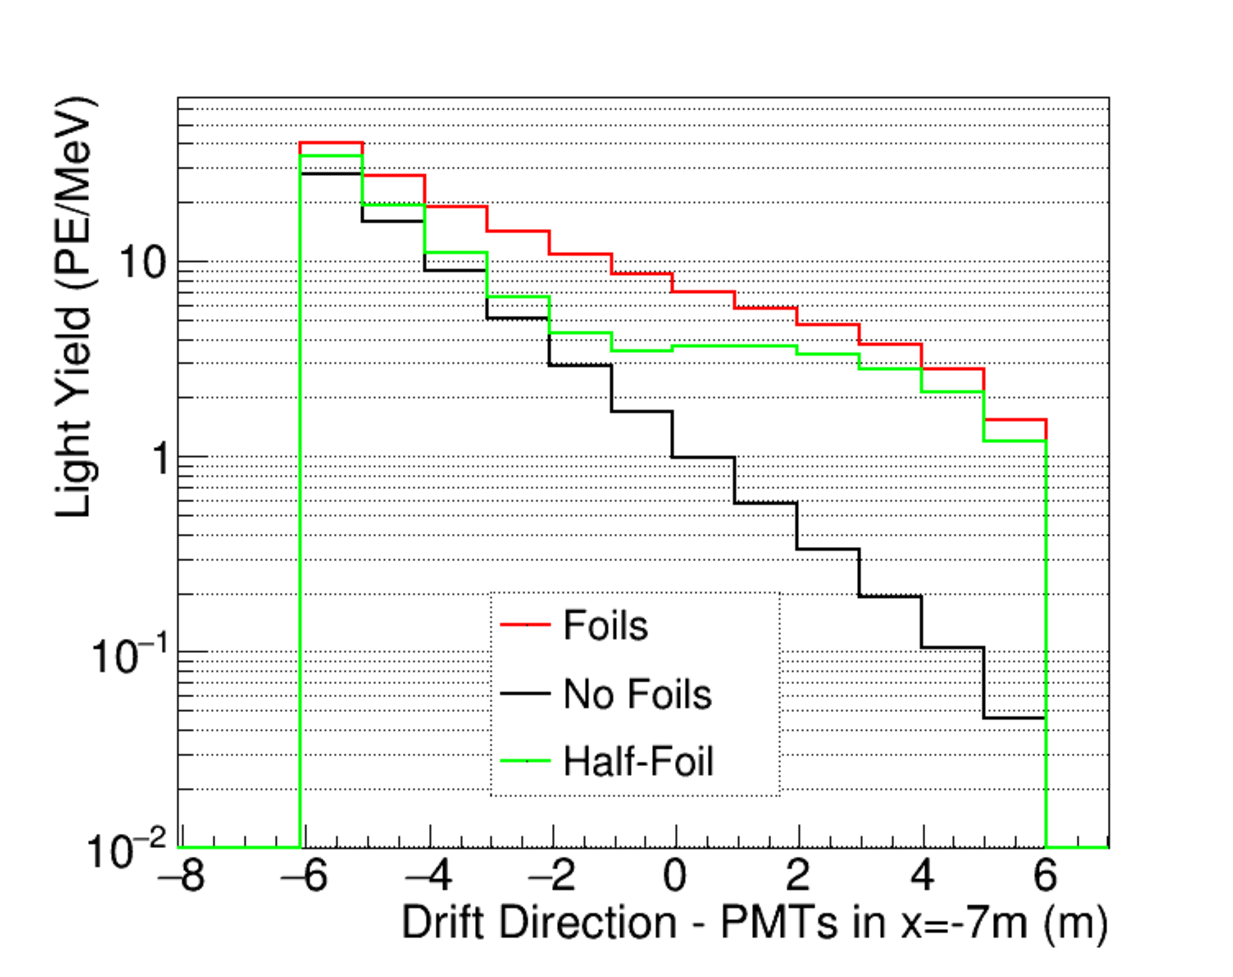
\includegraphics[width=0.49\textwidth]{graphics/dppd_PhotLibProjectionComparison_Drift.pdf}} \hfill
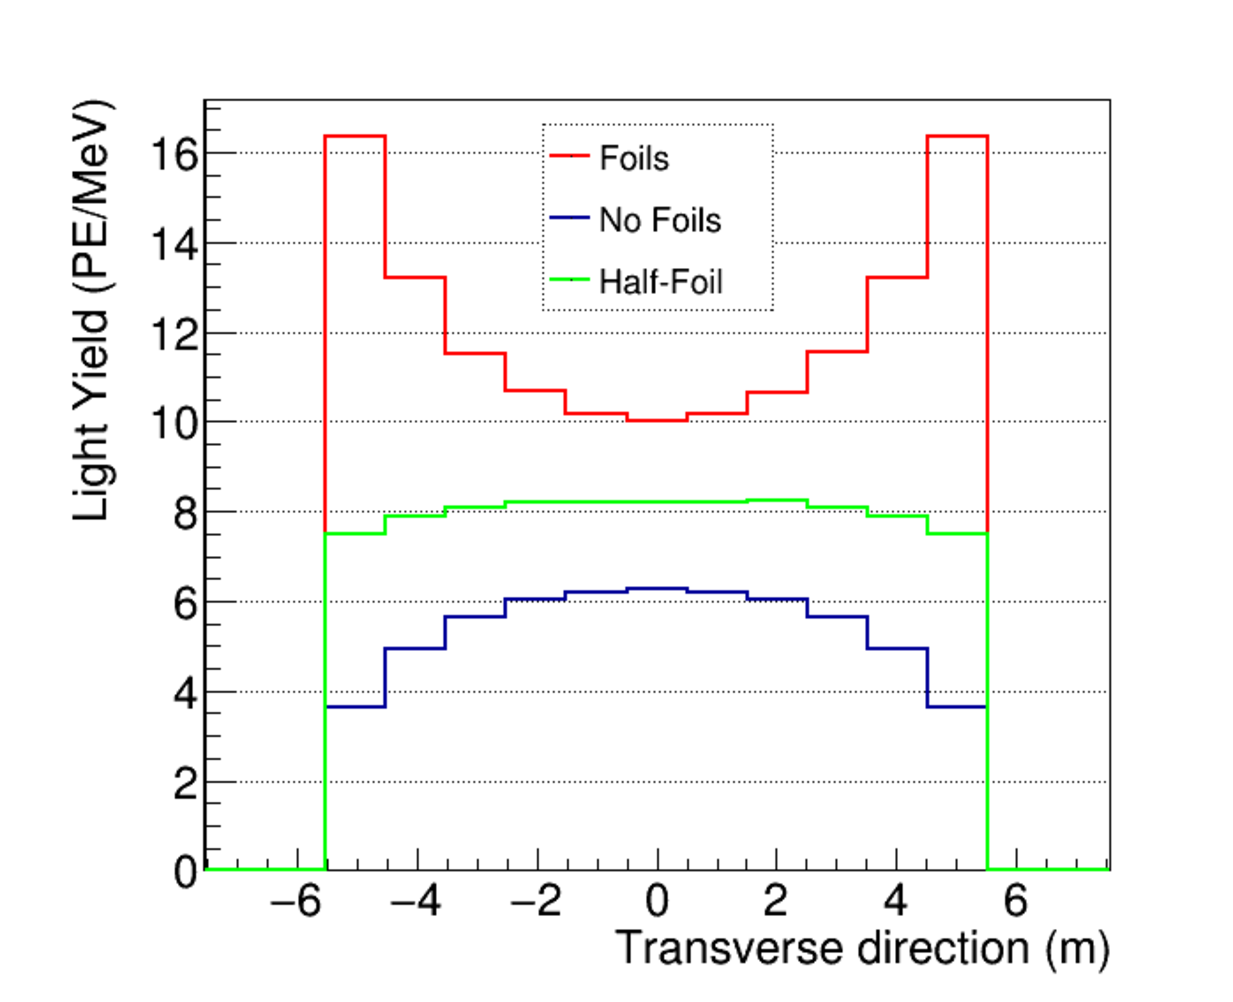
\includegraphics[width=0.49\textwidth]{graphics/dppd_PhotLibProjectionComparison_Trans.pdf}
\end{dunefigure}

We can also see the effect of the \dword{wls} reflector foils on the expected light yields in Fig.~\ref{fig:dppd_fd_light_yield_comparisons}, where the yields are shown as a function of the drift coordinate (left panel) and transverse coordinate (right panel), and averaging over the two other spatial coordinates. The drift coordinate is the vertical one, while the transverse coordinate is the horizontal direction perpendicular to the neutrino beam direction. The left panel provides better appreciation of the main trend in the spatial response, namely the light yield reduction with increasing distance from the cathode. The \dword{wls} reflector foils are particularly useful in improving the yields at small drift distances, where the yields are lower. The foils reduce the very large non-uniformity in spatial response between cathode and anode by more than one order of magnitude. The full foils geometry provides better yields than half foils in the lower half of the detector. The difference between the two geometries is less significant at small drift distances. Being the most inefficient region of the \dword{pds}, the latter is the most important one to optimize through foils. In addition, the right panel shows that the half foils geometry is the one providing the best uniformity along the transverse direction. These plots justify why the half \dword{wls} foils geometry has been selected for the \dword{pds} baseline design.     

\begin{dunefigure}[Expected 2D light yield in the full \dword{dp} \dshort{fd} cryostat.]{fig:dppd_fd_light_yield}
{Expected light yield in the full \dword{dp} \dshort{fd} cryostat, for the half \dword{wls} reflector foils geometry. The yield units are number of photo-electrons per \si{\MeV} of deposited energy. The 2D yield is shown as a function of the drift (vertical axis) and transverse (horizontal axis) directions, averaging over the third spatial coordinate (not shown). The red contours indicate the \dshort{tpc} active volume. The \dwords{pmt} are located at a drift coordinate of \SI{-7}{\m}.}
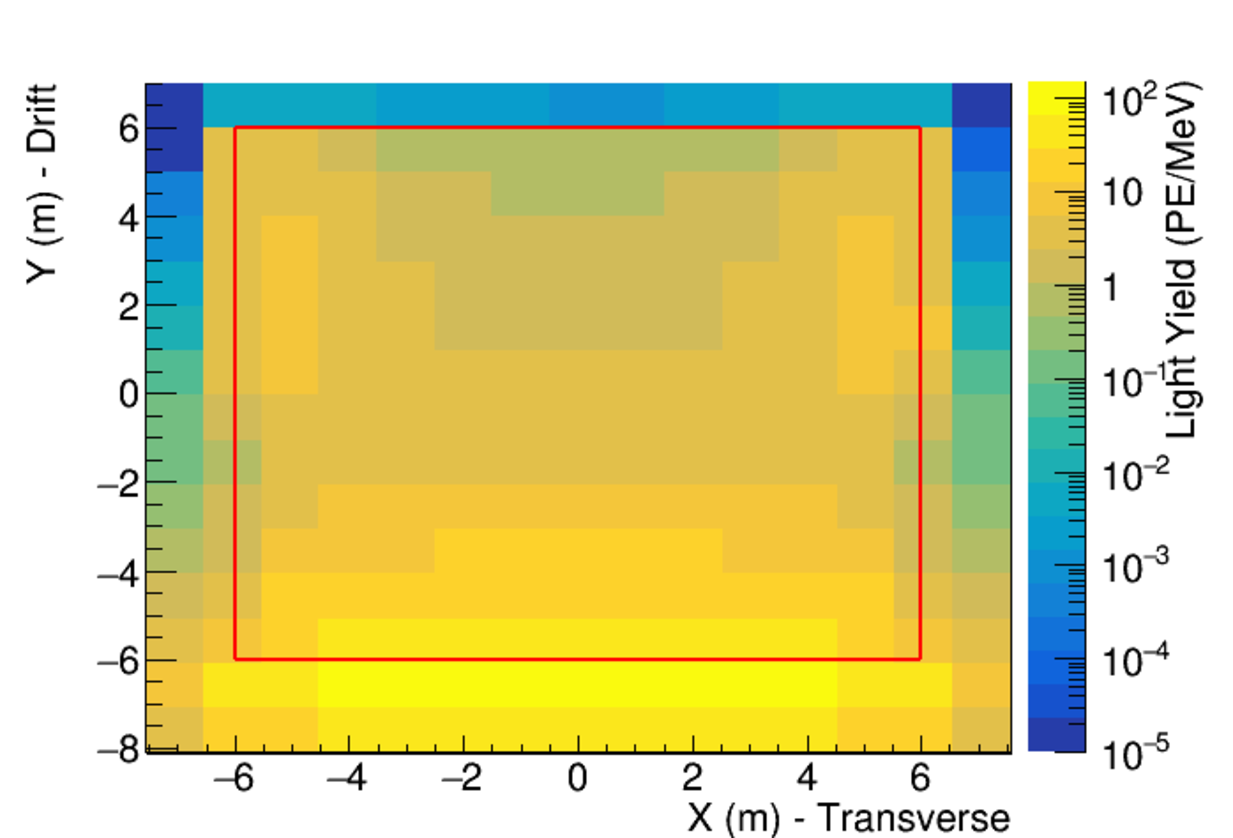
\includegraphics[width=0.65\textwidth]{graphics/dppd_PhotLibHalfFoil_longuerrange.pdf} 
\end{dunefigure}

Figure~\ref{fig:dppd_fd_light_yield} shows the detected light yield, for the half foils baseline geometry, as a function of drift and transverse directions simultaneously, and averaging over the beam direction. Near the cathode plane ($Y=$\SI{-6}{m} in this figure) the highest light yield is expected near the center of the active volume ($X=0$). The opposite is true near the anode plane ($Y=$\SI{+6}{m}).  


\section{Validation with Data from Photon Detector System Prototypes}
\label{sec:fddp-pds-prototypes}



\section{Baseline Design Validation and Projected Photon Detector Performance}
\label{sec:dp-pds-performance}

After the initial simulation studies described in the \dshort{tp} \cite{Abi:2018rgm}, we have progressed toward a more realistic understanding of the projected \dshort{pds} performance using the \dshort{larsoft} framework:
%
\begin{itemize}
\item Optical simulations are now performed in the \dword{dp} \dword{fd} module geometry. In the \dword{fd} \dshort{tp}, physics studies assumed the \dword{pddp} geometry. Considering the lack of any optical segmentation in the \dword{dp} design, light is simulated in the full \dpactivelarmass \dshort{tpc} active volume. Simulation assumptions for light generation and light transport are described in Section~\ref{subsec:dp-pds-simulation_assumptions}. For each of the \dpnumpmtch \dwords{pmt}, simulations take into account how the photon detection probabilities and the photon propagation times vary throughout the \dshort{tpc} active volume.
%
\item The electronics response and the reconstruction of optical hits and optical clusters has been simulated. Simulation assumptions for light detection by the \dwords{pmt} are also described in Section~\ref{subsec:dp-pds-simulation_assumptions}. Optical hits are the reconstructed optical signals on single \dshort{pmt} waveforms and are characterized by a hit time, amplitude, and charge. Optical hits must have an amplitude of at least \SI{10}{ADC counts} above baseline. Optical clusters refer to a collection of \dshort{pmt} hits correlated in time and space. They are typically induced by the same underlying flash of scintillation light in \lar. The parameters of the clustering algorithm are discussed later in this section.

%
\item The physics studies now also include radiological backgrounds. Simulating radiological backgrounds is critical in realistically optimizing the optical reconstruction parameters. The radiological model includes several radio-isotopes throughout the \lar volume, with \SI{1.01}{\becquerel/\kg} of $^{39}$Ar providing the most activity. In addition, an impinging neutron flux of \SI{e-5}{\cm$^{-2}$\s$^{-1}$} is accounted for.
\end{itemize} 

Expected \dword{pds} light yields in the \dword{pddp} and \dword{dp} \dword{fd} module geometries are discussed in Section~\ref{subsec:dp-pds-simulation_yields}

%%%%%%%%%%%%%%%%%%%%%%%%%%%%%%%%%%%%%%%%%%%%%%%%%%%%%%%%%%%%%%%%%%%%

\subsection{Event $t_{0}$ Reconstruction}
\label{subsec:dp-pds-performance_t0}

As discussed in Section~\ref{sec:dp-pds-requirements}, event $t_0$ reconstruction for non-beam events via the \dshort{pds} is particularly important to fiducialize nucleon decay candidates in \dword{dune}. Proton decay signal events with a %\ptoknubar 
$p\rightarrow K^{+} \bar\nu$ final state have been simulated with GENIE \cite{Andreopoulos:2009rq} throughout the \dword{dp} \dshort{tpc} active volume, and their optical clusters were reconstructed using the full simulation and reconstruction chain. \dword{ndk} events should deposit approximately \SI{400}{\MeV} visible energy in the \lar. The same reconstruction algorithm has also been applied to the simulated radiological backgrounds. In a first cluster reconstruction step, three parameters are optimized to group optical hits into separate clusters:
%
\begin{description}
\item[Maximum cluster duration:] maximum time difference among all \dshort{pmt} hits in the cluster.
\item[Maximum hit time distance:] maximum time difference between successive \dshort{pmt} hits in the cluster. By definition, this quantity is smaller than, or equal to, the maximum cluster duration.
\item[Maximum hit distance:] maximum spatial distance between neighbouring \dshort{pmt} hits in the cluster. 
\end{description}

For each chosen set of parameters (maximum cluster duration, maximum hit time distance, maximum hit distance), a threshold for minimum cluster charge (in \dwords{pe}) is defined, so a fixed, and tolerable, radiological background rate above threshold and per \SI{8}{\milli\s} maximum drift time is obtained. The chosen parameters are those that maximize the efficiency of detecting a \dword{ndk} cluster higher than this minimum cluster charge. For the \dword{pds} baseline design with half foils, the optimal values for the maximum cluster duration, maximum hit time distance and maximum hit distance were found to be \SI{100}{\ns}, \SI{100}{\ns} and \SI{5.5}{\m}, respectively. In other words, optical hits belonging to the same cluster are required to be nearly coincident in time, but only loosely correlated in space. As expected, it was also found that this optimization process yields a different result for a no foil \dword{pds} configuration, where light is more concentrated in space. 

After clustering optical hits as described above, and without applying any threshold on cluster charge, several optical clusters per event are reconstructed. At this stage, any deposit resulting in at least one optical hit is reconstructed by the \dshort{pds}, giving negligible \dword{ndk} optical cluster inefficiency but very high radiological background cluster multiplicity per event. 

In a second optimization step, we define the $t_0$ candidate clusters in the event as the ones fulfilling one additional condition: {\bf cluster spatial position}.

Albeit much less accurate than the \dshort{tpc} response, the \dshort{pds} response also provides some spatial information about the event in the plane perpendicular to the drift direction. The position of the $t_0$ candidate cluster in the plane perpendicular to the drift must be within \SI{1.5}{\m} of the simulated \dword{ndk} decay vertex\footnote{The matching in position with the MC truth information is of course only possible in simulations. However, we expect the \dshort{tpc} imaging performance to be so superior to the \dshort{pds} one that matching \dshort{pds} position with MC truth position is essentially equivalent to matching \dshort{pds} position with \dshort{tpc} reconstructed position.}. Because radiological clusters are randomly distributed with respect to the \dword{ndk} vertex, this position matching provides a strong background cluster suppression of about two orders of magnitude.

We define the {\bf \dword{ndk} $t_0$ reconstruction efficiency} as the efficiency to reconstruct at least one $t_0$ candidate cluster associated to the \dword{ndk} energy deposit. As shown below, the cluster spatial position requirement causes some inefficiency for events farther from the \dshort{pds} because of poorly reconstructed cluster spatial position in the plane perpendicular to the drift.

In general, several $t_0$ candidate clusters will be reconstructed per event, induced by the \dword{ndk} signal, by radiological activity, and by \dshort{pmt} dark counts. If more than one choice exists, event $t_0$ information is associated to the $t_0$ candidate cluster of highest charge. For events where at least one $t_0$ candidate cluster exists, we define the {\bf \dword{ndk} $t_0$ reconstruction purity} as the probability for the highest charge $t_0$ candidate cluster in the event to be associated with the \dword{ndk} signal. A purity value $<1$ can be obtained if the highest charge $t_0$ candidate cluster is due to radiological activity. The choice of the $t_0$ candidate cluster with the highest charge is made to maximize purity because radiological clusters have, on average, fewer reconstructed \dwords{pe} per cluster. As discussed in Section~\ref{sec:dp-pds-requirements}, we require a high purity to minimize $t_0$ reconstruction ambiguities.
%

\begin{dunefigure}[Optimization of $t_0$ candidate cluster spatial position reconstruction for \dword{ndk} events.]{fig:dppd_ndk_optimization}
{Efficiency, purity, and efficiency times purity for the $t_0$ candidate cluster to be correctly associated to the \dword{ndk} energy deposit, as a function of the maximum 2D distance between the \dshort{pds}-reconstructed position of the $t_0$ candidate cluster and the actual \dword{ndk} vertex, in the plane perpendicular to drift. A maximum distance of \SI{1.5}{\m} optimizes the product of efficiency times purity.}
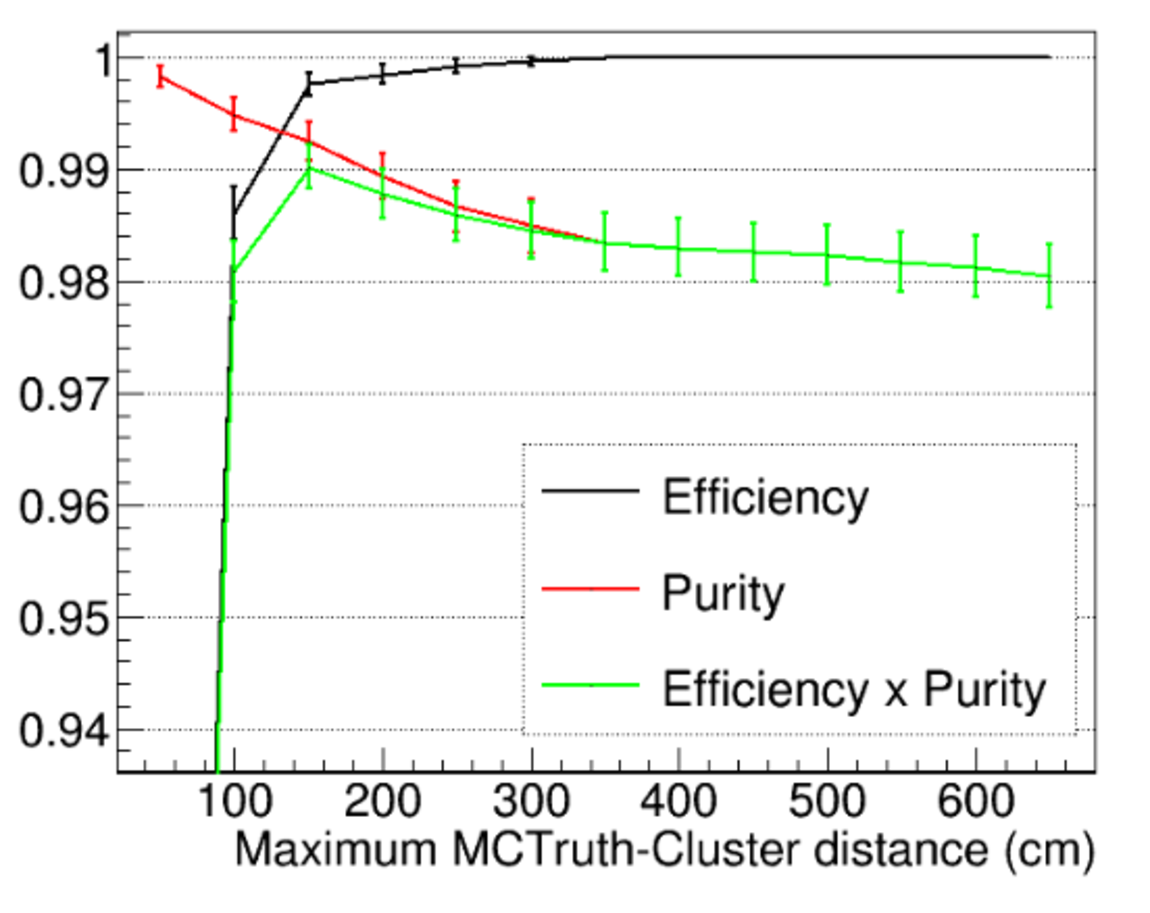
\includegraphics[width=0.5\textwidth]{graphics/dppd_ndk_optimization.pdf}
\end{dunefigure}

Figure~\ref{fig:dppd_ndk_optimization} illustrates how the \dword{ndk} signal efficiency, purity, and efficiency$\times$purity averaged over the entire \dshort{tpc} active volume vary as a function of the maximum 2D distance between the $t_0$ candidate cluster reconstructed position and the \dword{ndk} vertex actual position in the plane perpendicular to drift. A maximum distance of \SI{1.5}{\m} optimizes the product of efficiency$\times$purity. For this optimal distance, an average efficiency value of \num{99.8}\% and purity value of \num{99.2}\% are obtained.  

Figure~\ref{fig:dppd_ndk_efficiency} shows how the \dword{ndk} $t_0$ reconstruction efficiency and purity vary as a function of the nucleon decay vertex distance from the cathode plane for the optimal cluster reconstruction parameters described above. Two configurations are compared: the proposed baseline design with half foils, and a design with no foils along the \dword{fc}. For the baseline design, both the efficiency and purity remain $>90\%$ throughout the \dword{tpc} active volume, satisfying the detector requirements laid out in Sec.~\ref{subsec:dp-pds-requirements_requirements}. From Figure~\ref{fig:dppd_fd_light_yield_comparisons}, a light yield of \SI{1}{PE/\MeV} is expected at the anode plane in the half foil simulation. Because of this, the \dword{pds} minimum light yield required at the anode position is also \SI{1}{PE/\MeV} (see Table~\ref{tab:specs:just:DP-PDS}). 

On the other hand, for the no foil configuration, both efficiency and purity drop rapidly at large distances from the cathode. This is due to the marked reduction in the detected \dword{ndk} light yield as the energy deposition occurs at increasingly larger distances from the cathode, see Figure~\ref{fig:dppd_fd_light_yield_comparisons}. In this case, the efficiency (purity) remains $>90\%$ only for distances up to \SI{10}{\m} (\SI{7}{\m}) from the cathode. This large improvement in efficiently and accurately reconstructing event $t_0$ information for \dword{ndk} events is the main, but not only, motivation to introduce reflector/\dword{wls} foils along the \dword{fc} walls in the baseline design.

\begin{dunefigure}[Nucleon decay $t_0$ reconstruction efficiency and purity.]{fig:dppd_ndk_efficiency}
     {Nucleon decay $t_0$ reconstruction efficiency (left panel) and purity (right), defined in text, as a function of decay vertex distance from the cathode. Two \dword{pds} designs are compared: no foils and half foils (baseline). The anode plane is at a drift position of \SI{+600}{\cm}, the cathode plane at a drift position of \SI{-600}{\cm},  and \dshort{pmt} plane is at a drift position of \SI{-700}{\cm}.}
    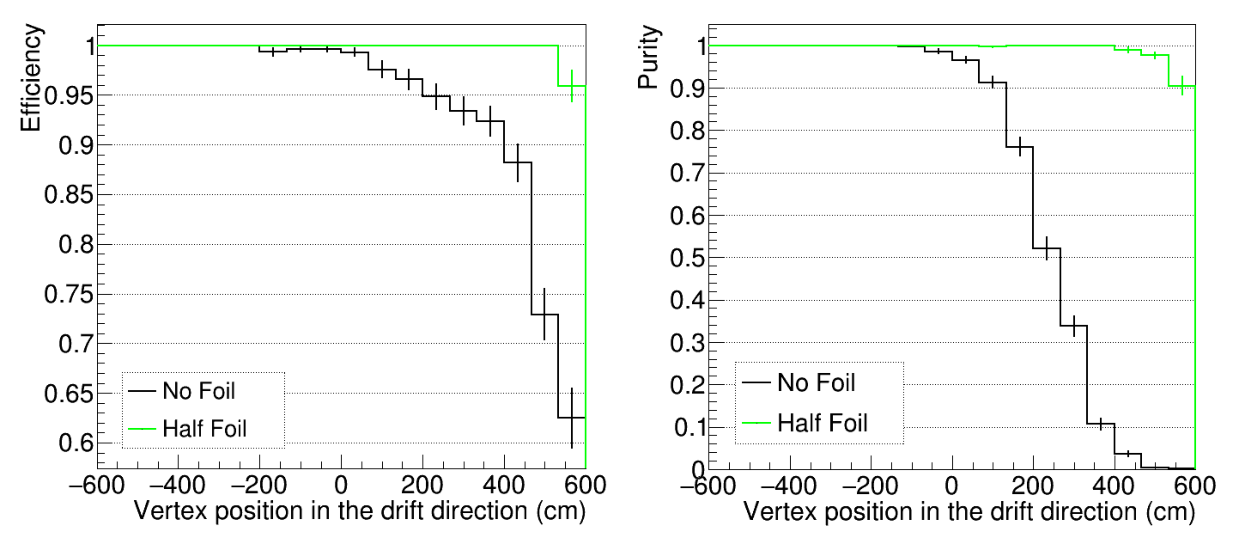
\includegraphics[width=0.90\textwidth]{graphics/dppd_ndk_efficiency.pdf}
    \end{dunefigure}

%%%%%%%%%%%%%%%%%%%%%%%%%%%%%%%%%%%%%%%%%%%%%%%%%%%%%%%%%%%%%%%%%%%%

\subsection{Supernova Burst Triggering}
\label{subsec:dp-pds-performance_trigger}

We have also studied how well the \dword{dp} \dshort{pds} triggers on an \dword{snb} occurring in our galactic neighbourhood. As described in Section~\ref{sec:dp-pds-requirements}, this is one of the primary goals of the \dword{pds}. To this end, \dword{snb} \nue \dword{cc} interactions have been generated with MARLEY \cite{marley} in our baseline \dword{pds} design with reflector/\dword{wls} panel assemblies installed in the top half of the \dword{fc}. In \dword{dune}, a real-time algorithm should provide trigger primitives by searching for \dshort{pmt} hits and optical clusters, where the latter combine several hits together based on their time/spatial information. Compared to the \dword{ndk} case, the reconstructed optical signals are much weaker because the typical deposited energies per \dword{snb} neutrino interaction are approximately \SI{20}{\MeV}. The online clustering process is similar to the offline cluster reconstruction discussed in Section~\ref{subsec:dp-pds-performance_t0}, albeit with some differences related to the lack of trigger information and detailed event reconstruction at this stage:
%
\begin{itemize}
\item Real-time optical clusters must have a minimum hit multiplicity to suppress clusters induced by radiological activity or \dword{pmt} dark counts. The higher the hit multiplicity, the lower the background cluster rate.
\item \dword{pds} spatial information is only used to group hits into separate clusters,  not to match \dword{pds} clusters with \dword{tpc} tracks in the plane perpendicular to the drift as in Section~\ref{subsec:dp-pds-performance_t0}.
\item Real-time optical clusters must be continuously reconstructed, while in Section~\ref{subsec:dp-pds-performance_t0}, only the \SI{7.5}{\milli\s} period preceding a charge-based trigger signal, corresponding to the maximum drift time, is considered.
\end{itemize}
%
In this case, the optimal real-time cluster reconstruction parameters, including a minimum hit multiplicity per cluster requirement, yield a \SI{0.05}{\Hz} radiological background cluster rate for an \dword{snb} \nue \dword{cc} signal cluster efficiency of \SI{11.8}{\%}. Once the optimal cluster parameters are found, the computation of the \dshort{pds}-based \dword{snb} trigger efficiency as a function of \dword{snb} distance is performed as follows:

\begin{itemize}
\item First, the minimum number of reconstructed clusters required in a \SI{2}{\s} time window  to issue a trigger is found\footnote{A \SI{2}{\s} time window was found to be optimal and is assumed throughout this section.}. The minimum cluster multiplicity is set by the requirement of one fake trigger per month at most (see Section~\ref{sec:dp-pds-requirements}) and by the radiological background cluster rate. The higher the background cluster rate, the higher the minimum cluster multiplicity must be to meet the $<$\num{1}/month fake trigger rate requirement. As mentioned above, the clustering optimization procedure yields a background cluster rate of \SI{0.05}{\Hz} or, on average, \num{0.1} clusters per \SI{2}{\s} window. For such a background rate level, a minimum cluster multiplicity of $\ge$\num{3} per \SI{2}{\s} time window is required for a $<$\num{1}/month fake trigger rate.
%
\item Second, and given the cluster parameters and minimum cluster multiplicity defined in the first step, the \dword{snb} triggering efficiency as a function of the number of \dword{snb} interactions is computed. For a \SI{11.8}{\%} average efficiency of reconstructing single \dword{snb} \nue interactions with the \dshort{pds}, and a minimum cluster multiplicity of \num{3} to issue a trigger, approximately \num{3}/\num{0.118}$\simeq$ \num{25} interactions must occur in the \dword{fd} module and within \SI{2}{\s} to obtain a non-negligible trigger efficiency. 
%
\item Third, and finally, the \dword{snb} triggering efficiency as a function of \dword{snb} distance is obtained. We use the theoretical assumptions shown in Figure~\ref{fig:dppd_snbassumptions} to extract the number of \dword{snb} neutrino interactions in a \SI{2}{\s} time window and in one \dword{dp} \dword{fd} module as a function of \dword{snb} distance. The left panel of Figure~\ref{fig:dppd_snbassumptions} shows the time-integrated expected number of \dword{snb} neutrino interactions as a function of distance, while the right panel in Figure~\ref{fig:dppd_snbassumptions} shows the assumed time profile of the burst during the first \SI{10}{\s}. Several hundred \dword{snb} neutrino interactions are expected in one \dword{dp} \dword{fd} module for a \SI{10}{\kilo\parsec} distant \dword{snb}\footnote{It is customary to evaluate the performance of \dword{snb} detectors for a \dword{snb} distance of \SI{10}{\kilo\parsec}, as this is approximately the distance to the Galactic Center.}, and about half of them are expected within the first \SI{2}{\s}. Given our earlier estimate that about \num{25} interactions should be sufficient for a non-negligible trigger efficiency, clearly, the \dshort{pds} should provide high \dword{snb} trigger efficiency for an \dword{snb} at a \SI{10}{\kilo\parsec} distance.
\end{itemize}

\begin{dunefigure}[SN burst triggering assumptions.]{fig:dppd_snbassumptions}
     {Left panel: expected number of \dword{snb} \nue \dshort{cc} interactions in one \dpactivelarmass active mass DP module as a function of \dword{snb} distance. The different green lines indicate different \dword{snb} models. Right panel: expected time profile of the \dword{snb}.}
    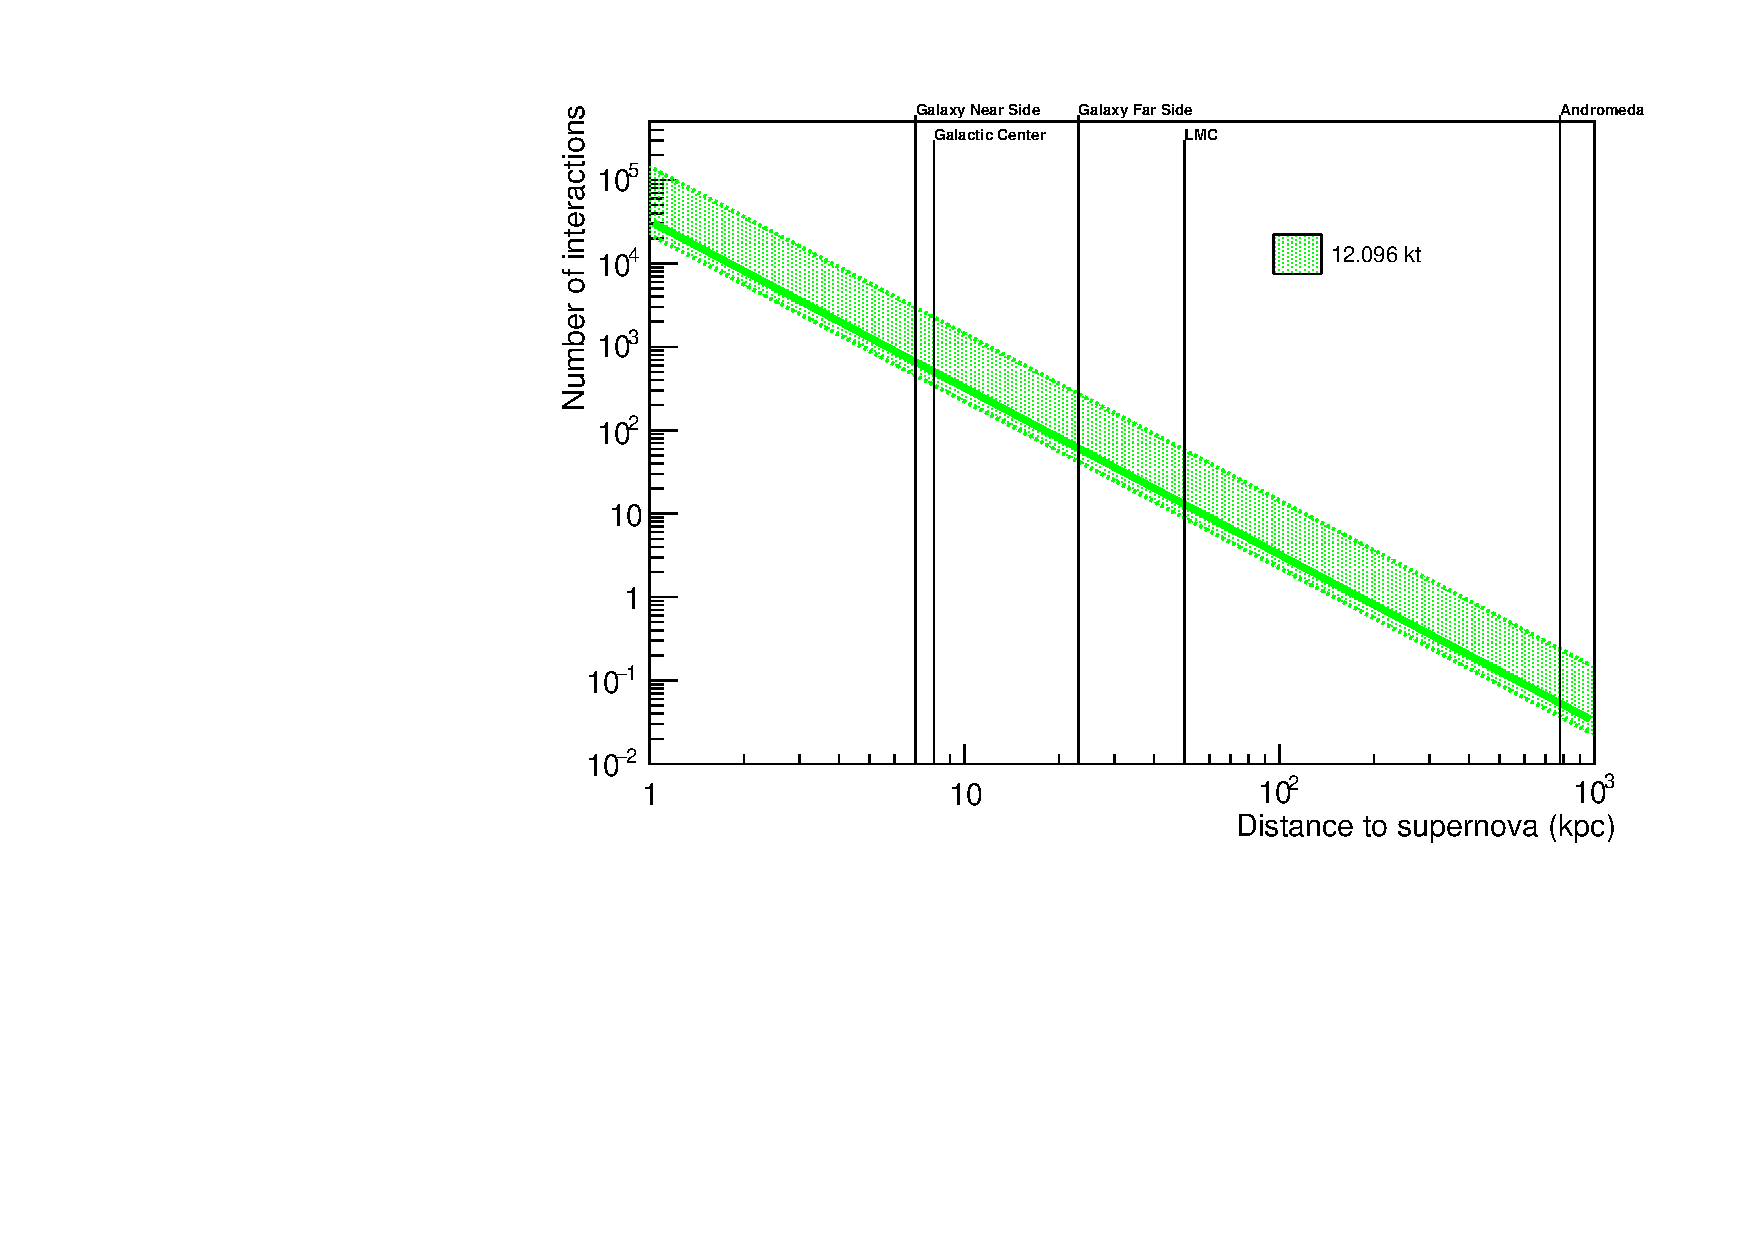
\includegraphics[width=0.49\textwidth]{graphics/dppd_events_vs_sndistance.pdf} \hfill
    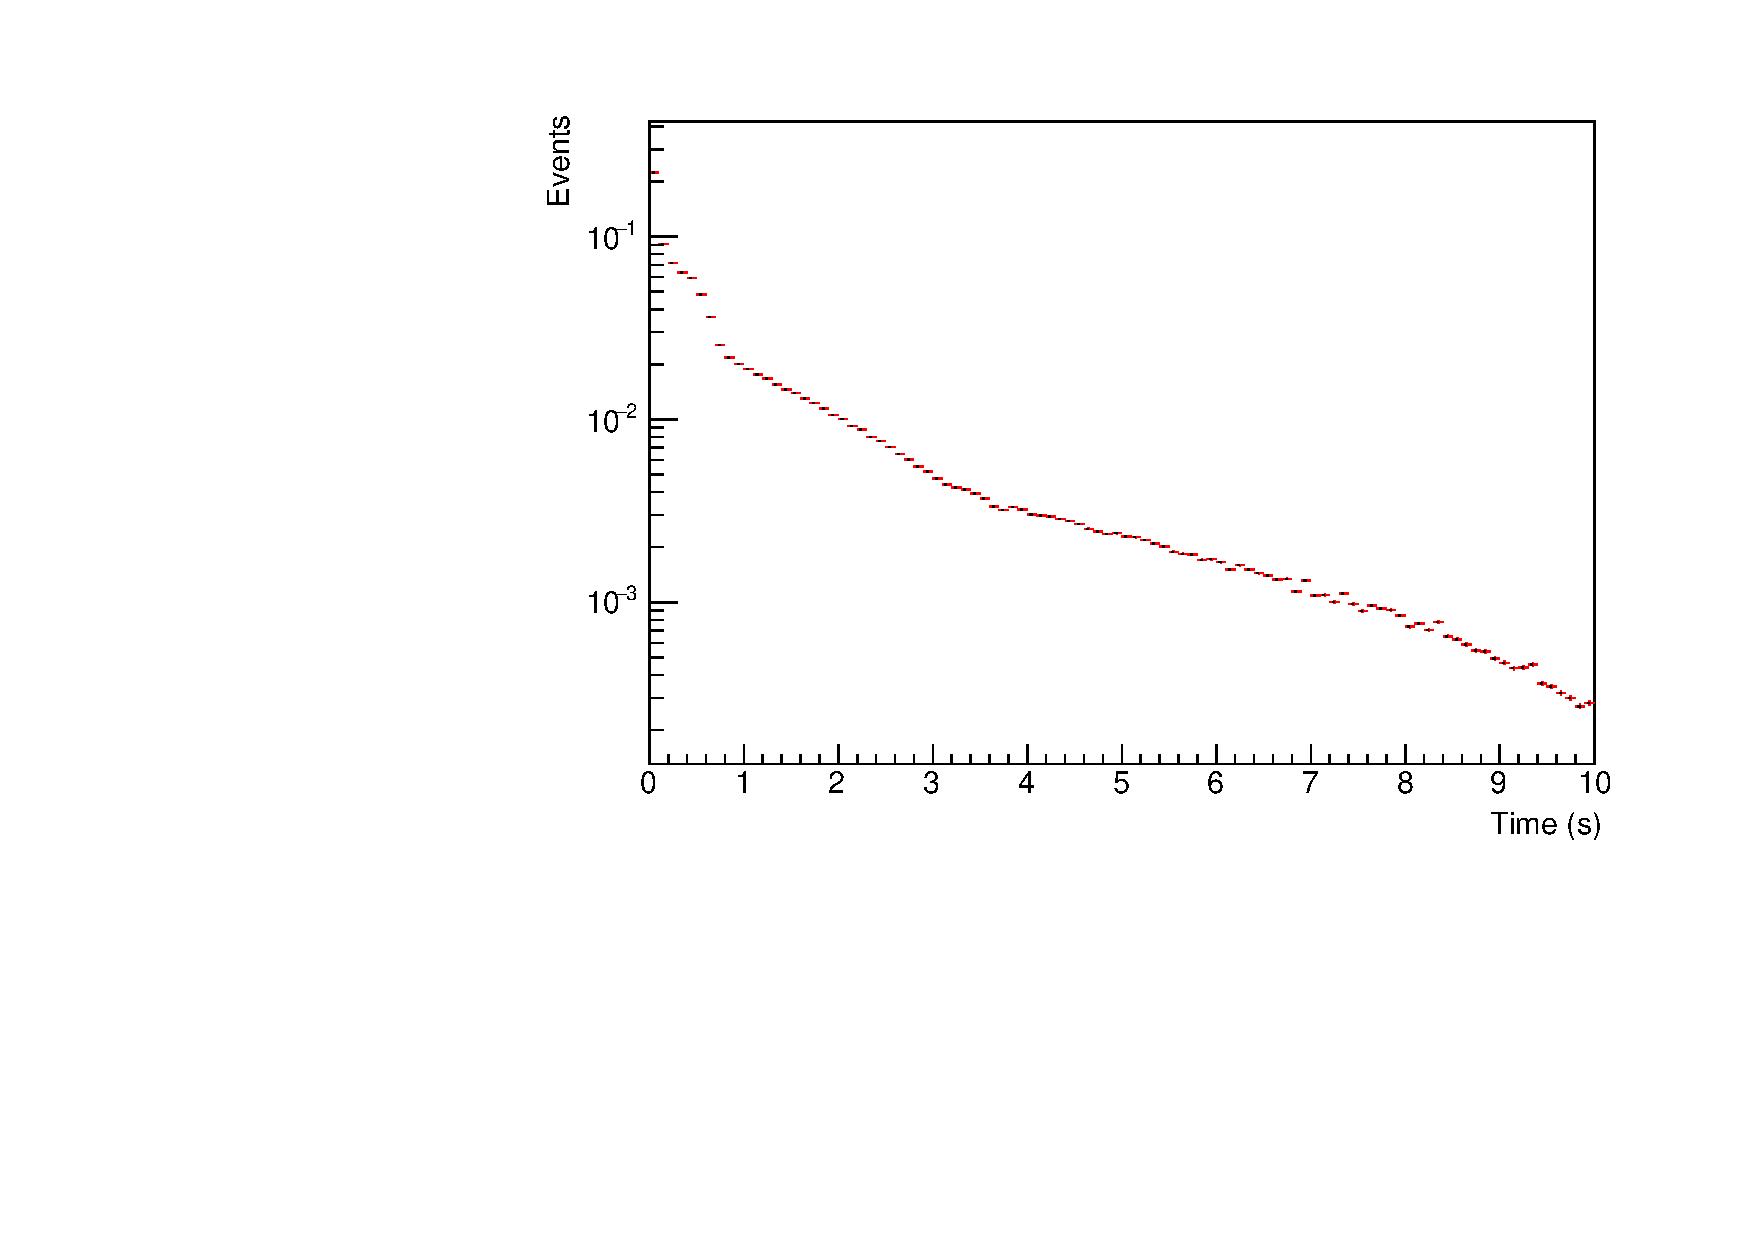
\includegraphics[width=0.49\textwidth]{graphics/dppd_sntime_profile.pdf} 
    \end{dunefigure}

The \dword{snb} triggering efficiency, computed following the procedure described above and as a function of \dword{snb} distance, is shown in Figure~\ref{fig:dppd_snbefficiency_vs_sndistance_half_foils}. The figure shows how the \dword{snb} triggering efficiency is affected by different choices in cluster reconstruction parameters. The best trigger efficiency found for the cluster parameters, yielding the lowest background cluster rate, is \SI{0.05}{\Hz}. In this case, a trigger efficiency in excess of \num{90}\% is obtained up to \dword{snb} distances of approximately \SI{25}{\kilo\parsec}. Therefore, the \dshort{pds} should yield a highly efficient trigger for \dword{snb} occurring anywhere in the Milky Way. 

\begin{dunefigure}[\dword{snb} triggering efficiency for different cluster reconstruction parameters.]{fig:dppd_snbefficiency_vs_sndistance_half_foils}
     {\dword{snb} triggering efficiency using \dword{dp} \dshort{pds} information as a function of \dword{snb} distance. Different curves indicate different choices of the optical cluster reconstruction parameters, resulting in different \dword{snb} \nue signal detection efficiencies (DE) and radiological background rates (BGR).}
    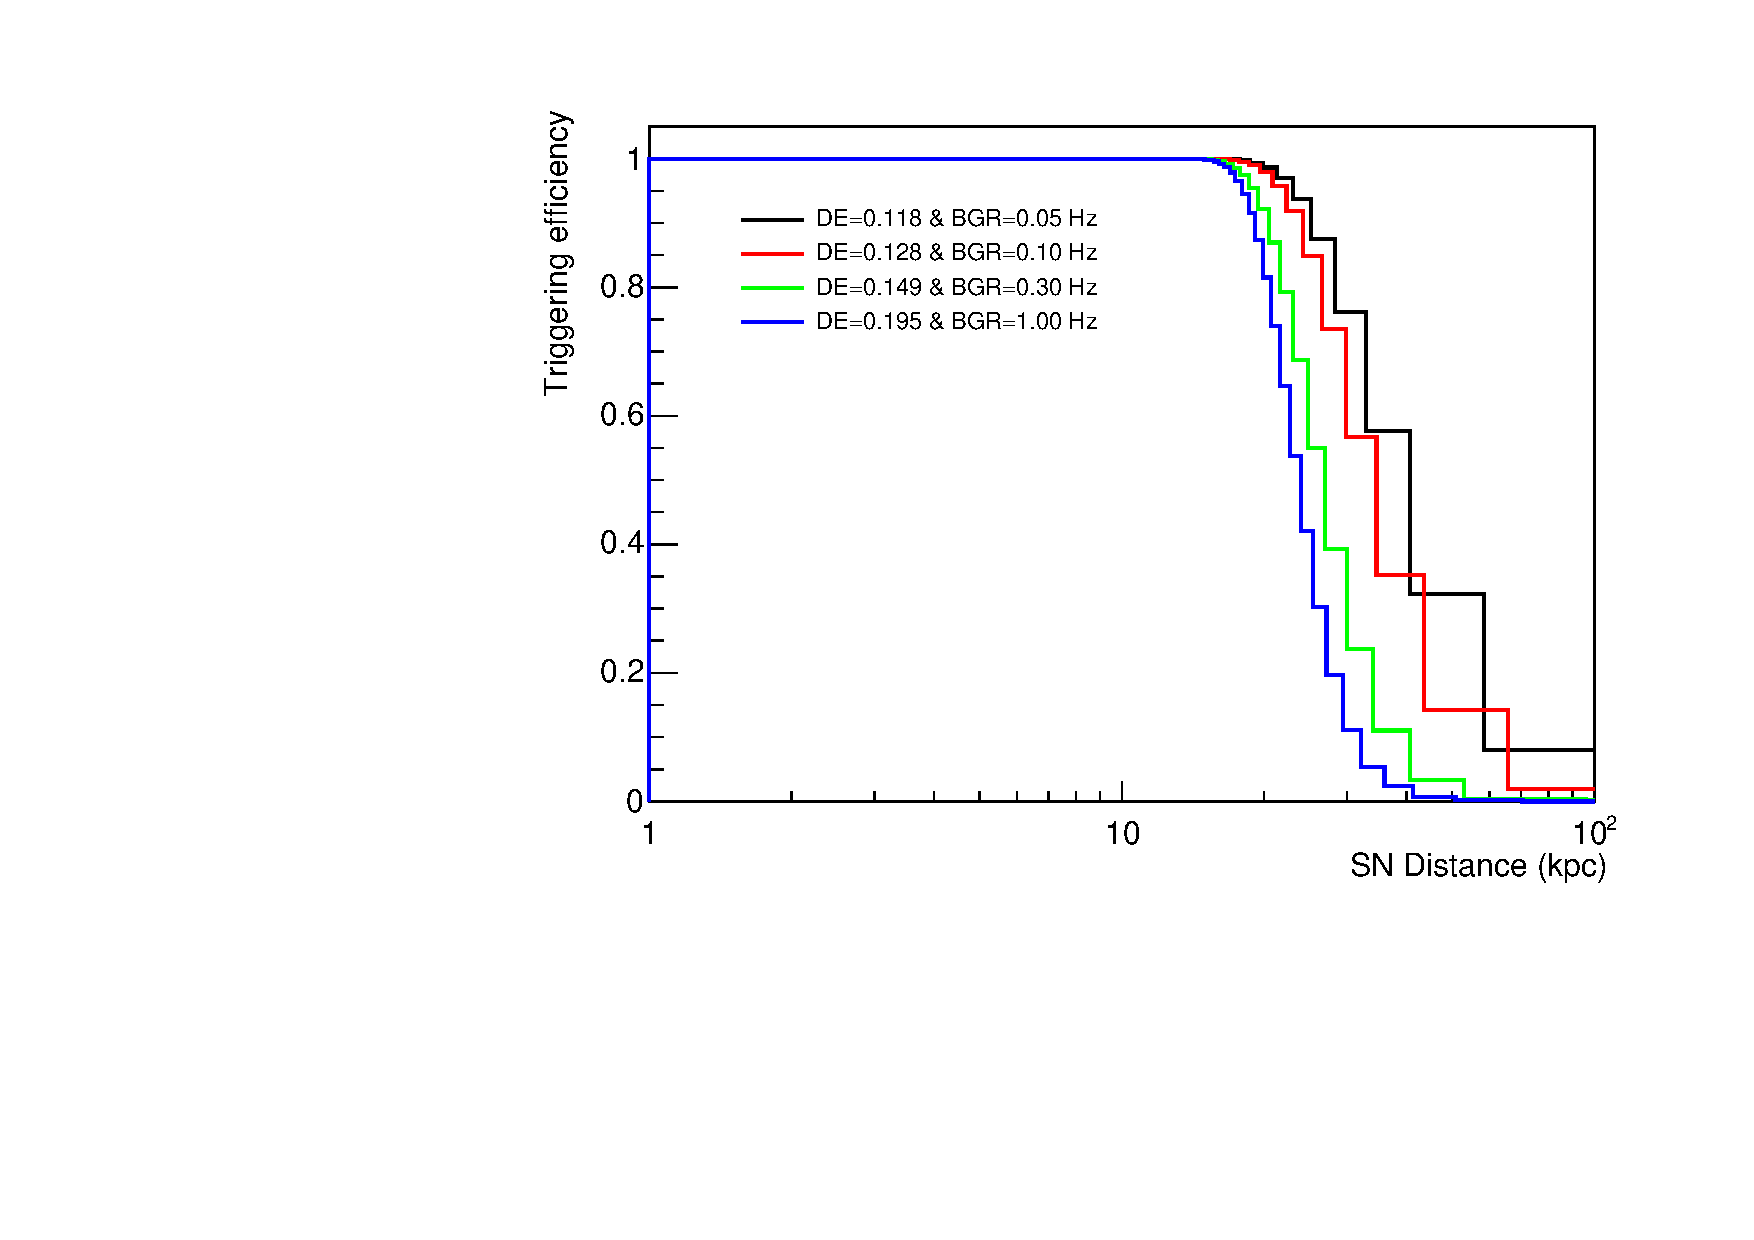
\includegraphics[width=0.6\textwidth]{graphics/dppd_snbefficiency_vs_sndistance_half_foils.pdf}
    \end{dunefigure}

Figure~\ref{fig:dppd_snbefficiency_vs_sndistance_comparison} shows how the \dword{snb} trigger efficiency of the baseline configuration with \dword{wls} reflector foils along the upper \dword{fc} half compares with alternative choices, namely no foils and full foils. Our minimum \dword{snb} trigger efficiency requirement of \num{90}\% at \SI{20}{\kilo\parsec} (see Sec.~\ref{subsec:dp-pds-requirements_requirements}) should be (barely) reachable even for the no foil configuration. In this case, the average light yield is expected to be about \SI{5}{PEs/MeV}, see Table~\ref{tab:dp-pds-light-yields}. For this reason, Table~\ref{tab:specs:just:DP-PDS} quotes \SI{>5}{\dwords{pe}/\MeV} as the average light yield requirement. On the other hand, the results improve noticeably with increased foil coverage, as $>$\num{90}\% trigger efficiency extends to approximately \num{25} and \SI{36}{\kilo\parsec} for the half foil and full foil configurations, respectively. 

\begin{dunefigure}[\dword{snb} triggering efficiency for different \dword{wls} foil configurations.]{fig:dppd_snbefficiency_vs_sndistance_comparison}
     {\dword{snb} triggering efficiency as a function of \dword{snb} distance for three different \dword{wls} foil configurations.}
    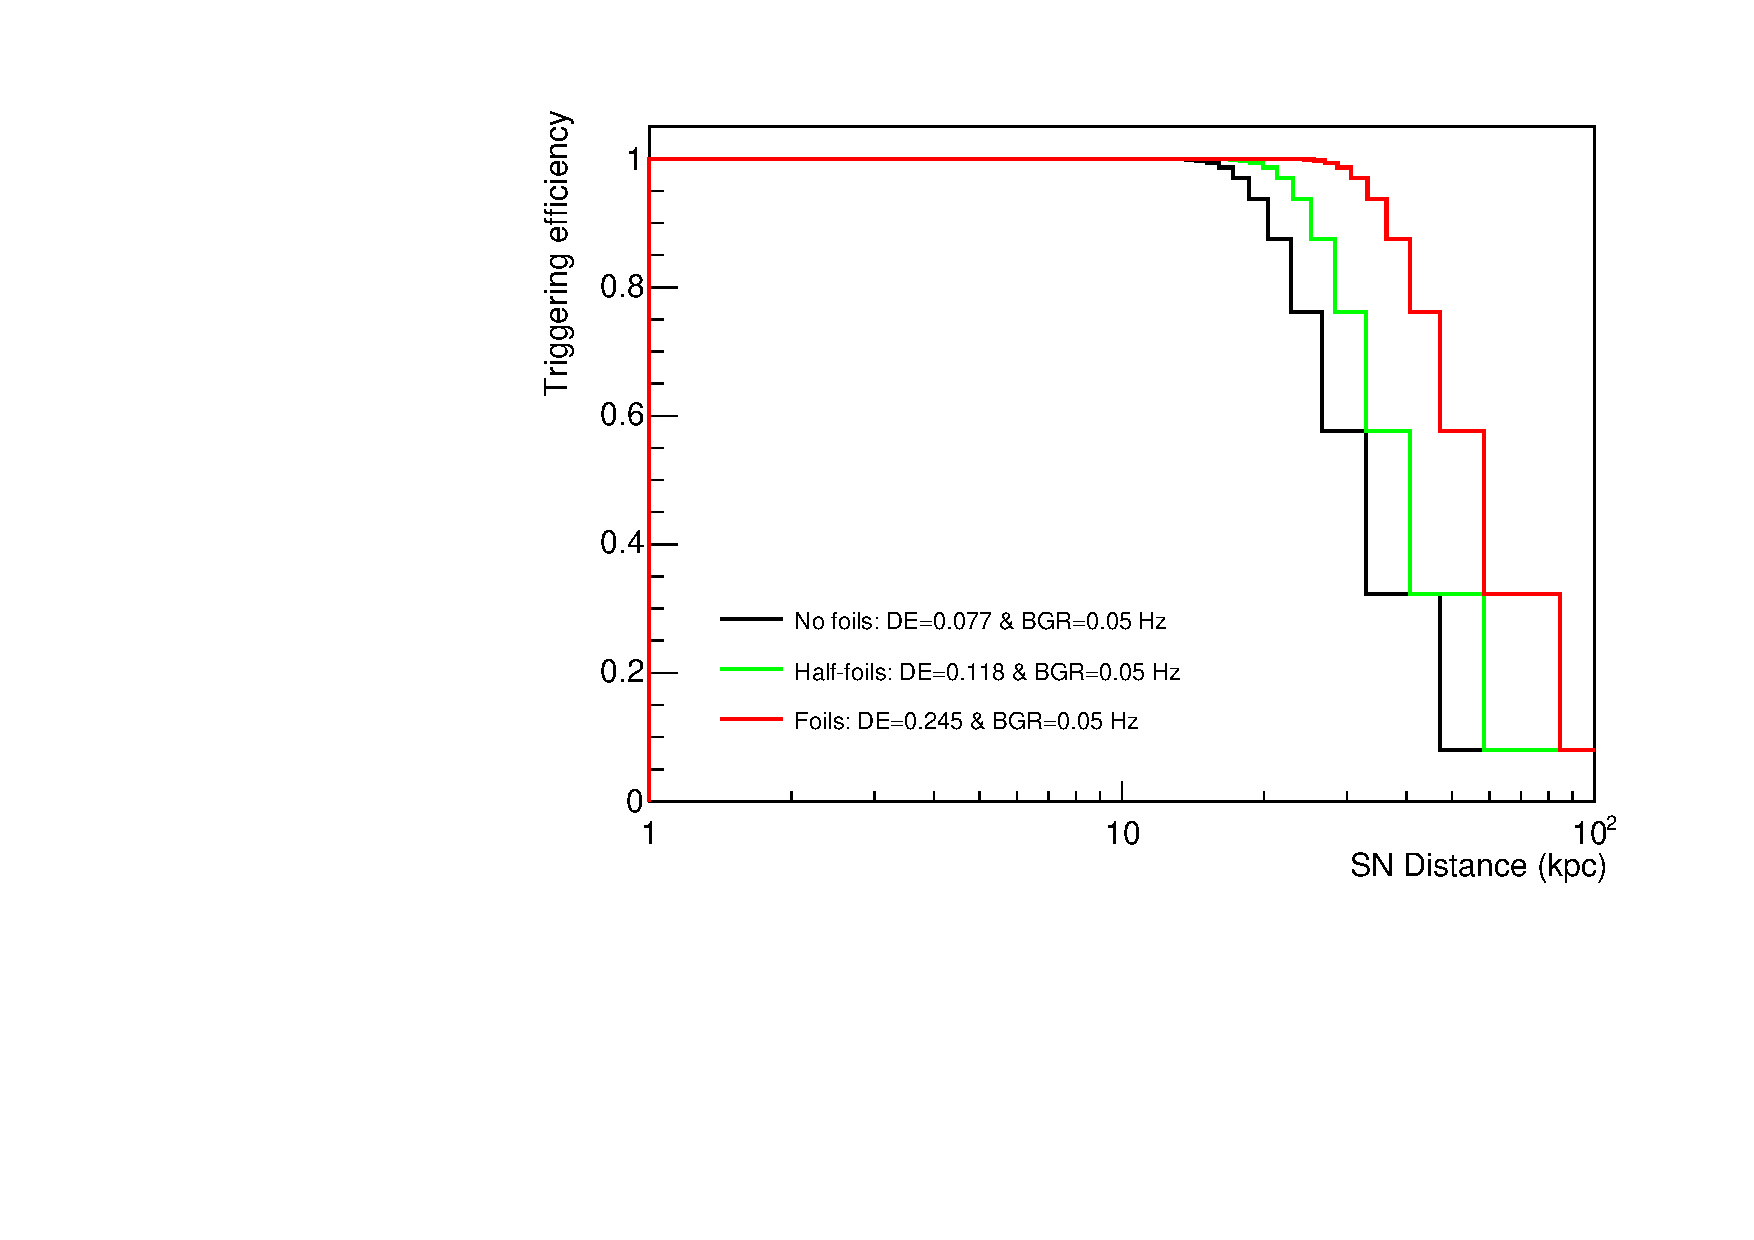
\includegraphics[width=0.6\textwidth]{graphics/dppd_snbefficiency_vs_sndistance_comparison.pdf}
    \end{dunefigure}

%%%%%%%%%%%%%%%%%%%%%%%%%%%%%%%%%%%%%%%%%%%%%%%%%%%%%%%%%%%%%%%%%%%%

\subsection{Event Energy Reconstruction}
\label{subsec:dp-pds-performance_calorimetry}

In addition to timing and triggering information, the \dword{pds} can also provide event energy information via the intensity of the reconstructed optical flashes. We focus in this section on beam neutrino interactions generated via the \dshort{genie} event generator \cite{Andreopoulos:2009rq}, as described in Section~\ref{subsec:dp-pds-requirements_requirements}.

A first requirement for a competitive energy reconstruction performance with the \dword{pds} is that optical hit saturation effects are kept to a manageable level by the \dword{pds} and associated readout electronics. Figure~\ref{fig:dppd_saturation} shows the expected average hit charge and average hit amplitude as a function of drift position of the neutrino interaction vertex for \SI{3}{\GeV} beam \nue \dshort{cc} interactions. For each event, the average is computed by considering hit \dshort{pds} channels only, that is, \dwords{pmt} detecting a charge of at least \SI{1}{PE}. The average hit charge per event is approximately \SIrange{50}{300}{} for \SI{3}{\GeV} beam \nue \dshort{cc} interactions throughout the \dword{tpc} active volume. The average charge is expressed in \dwords{pe}, with the average amplitude in \dwords{pe} per \SI{4}{\nano\s} time bin. This time bin width is comparable with the \SI{6}{\nano\s} timescale characteristic of the prompt scintillation light in \dshort{lar}. For events near the cathode plane, about \SI{300}{\dwords{pe}} per hit channel are detected, corresponding to a maximum amplitude over \SI{4}{\nano\s} of about \SI{50}{\dwords{pe}}. The factor of 6 difference between average charge and average amplitude is because only \SI{23}{\%} of the scintillation light is prompt and (to a smaller extent) because of additional time smearing introduced by light propagation to the same \dword{pmt} from different \dshort{lar} voxels containing energy deposits. From these plots, we conclude that the \dshort{pds} signal readout should withstand signal amplitudes of at least \SI{100}{\dwords{pe}} over \SI{6}{\nano\s} to mitigate saturation effects (see Table~\ref{tab:specs:just:DP-PDS}).

\begin{dunefigure}[Average charge and amplitude per hit channel in beam neutrino interactions.]{fig:dppd_saturation}
{Expected average hit charge (left panel, in \dwords{pe}) and average hit amplitude (right panel, in \dwords{pe} per \SI{4}{\nano\s} time bin) as a function of event drift position for \SI{3}{\GeV} beam \nue \dshort{cc} interactions. The scatter plots  contain one entry per event, and the average is for hit \dshort{pds} channels only.}
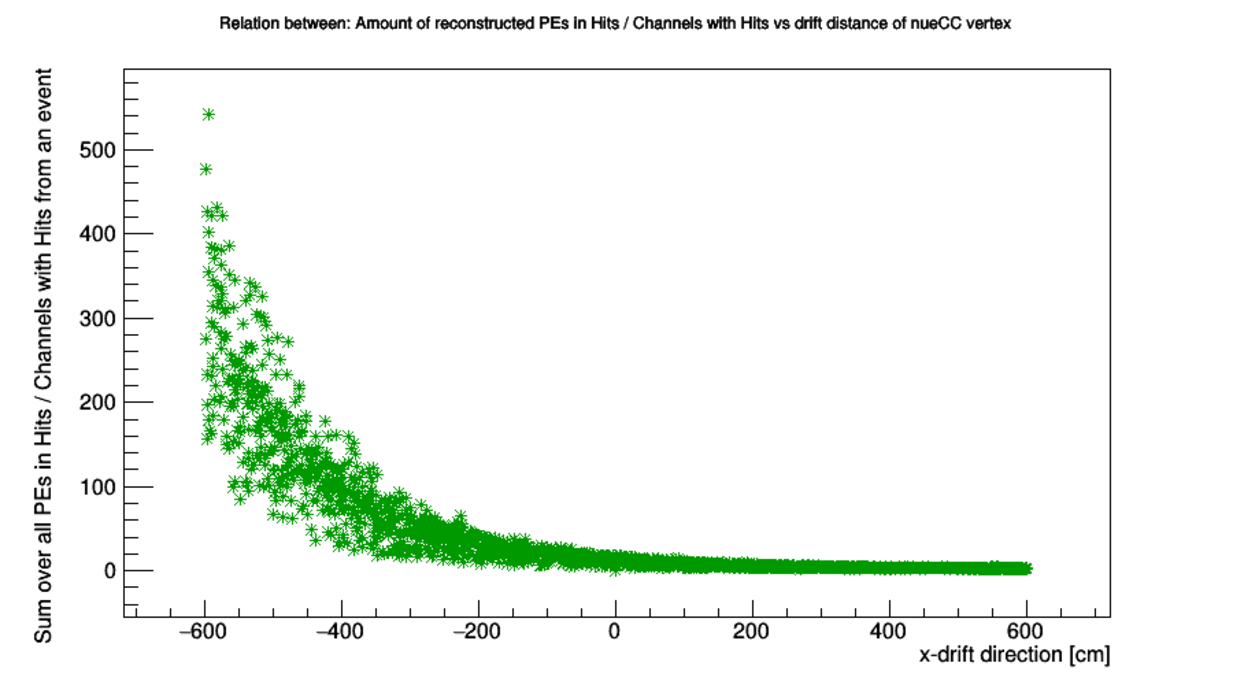
\includegraphics[trim={0cm 0cm 0cm 1.cm}, clip, width=0.49\textwidth]{graphics/dppd_avg_charge_per_channel.pdf} \hfill
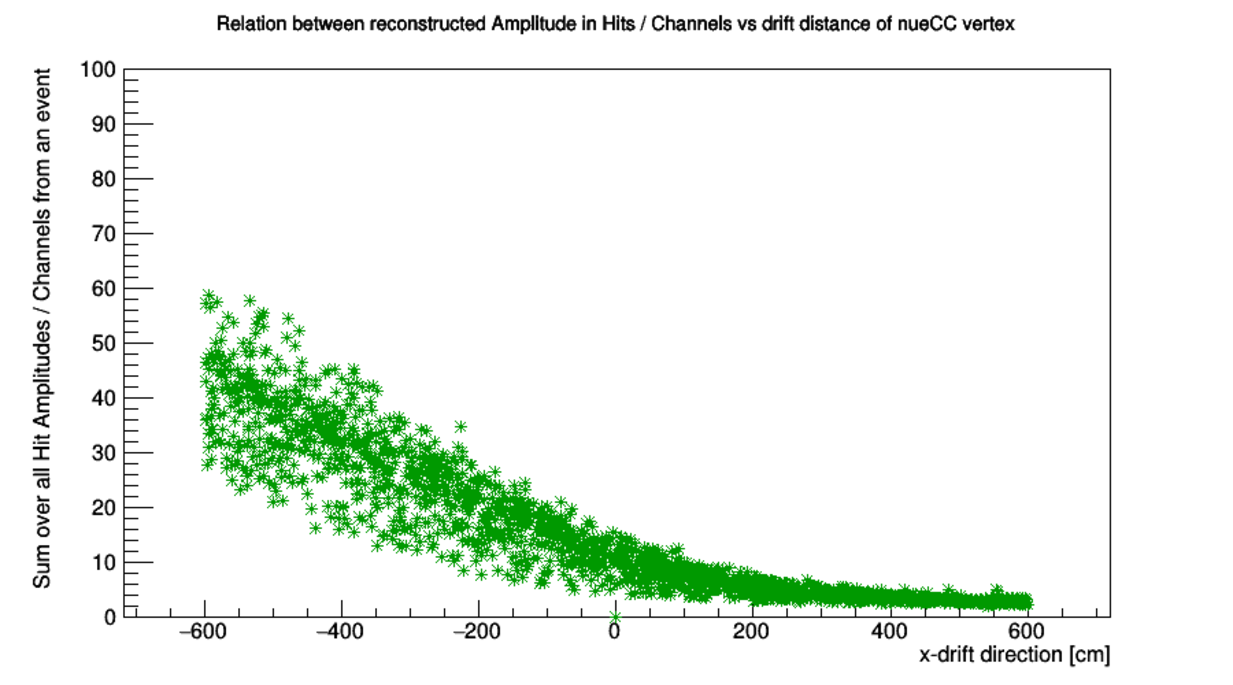
\includegraphics[trim={0cm 0cm 0cm 1.cm}, clip, width=0.49\textwidth]{graphics/dppd_avg_amplitude_per_channel.pdf}
\end{dunefigure}

The neutrino energy for the same \SI{3}{\GeV} beam \nue \dshort{cc} interactions has been reconstructed using \dword{pds} information as follows:
%
\begin{equation}
\label{eq:dppd_ereco} 
%    E_{\rm reco} = \frac{Q}{\varepsilon_{\rm \dword{pmt}}\cdot %V_{\dword{pds}}(\vec{x}_{\rm int})\cdot Y}
E_{\rm reco} = \frac{Q}{\varepsilon_{\rm PMT}\cdot V_{PDS}(\vec{x}_{\rm int})\cdot Y}
\end{equation}
%
\noindent where $Q$ is the total charge (in \dwords{pe}) of all \dword{pmt} hits reconstructed in the event, $\varepsilon_{\rm PMT}$ is the \dword{pmt} quantum efficiency, $V_{PDS}(\vec{x}_{\rm int})$ is the \dword{pds} visibility at the neutrino interaction vertex $\vec{x}_{\rm int}$, defined as the fraction of \lar scintillation photons that reach one of the \dword{pmt} photo-cathode surfaces, $Y=\SI{2.4e4}{photons/MeV}$ is the scintillation light yield, and $E_{\rm reco}$ is the resulting reconstructed energy. In Eq.~\ref{eq:dppd_ereco}, we include \dword{pmt} dark counts in time coincidence with the beam, and we assume that \dword{tpc} information will provide the neutrino interaction vertex information that is needed for the visibility estimate. The event energy reconstructed in this way is shown in the right panel of Fig.~\ref{fig:dppd_beam_calorimetry}, for a sample of neutrino interactions occurring in the \lar fiducial volume. The distribution peaks at about \SI{2.2}{GeV}, somewhat lower than the generated neutrino energy of \SI{3}{GeV}. A gaussian fit to this distribution yields about a \num{20}\% resolution. This value meets the requirement described in Sec.~\ref{subsec:dp-pds-requirements_requirements}, and confirms that the \dword{pds} should be able to provide energy information that is competitive with the \dune \dword{tpc}. Figure~\ref{subsec:dp-pds-requirements_requirements} also shows, in the left panel, the true deposited energy $E_{\rm depo}$ in the \lar active volume for the same simulated events. This distribution shows how an ideal detector could reconstruct event energy, for beam neutrino events. From the comparison of $E_{\rm depo}$ and $E_{\rm reco}$, we conclude that a significant portion of the bias and smearing seen in $E_{\rm reco}$ is already present at the $E_{\rm depo}$ level, and hence cannot be corrected for in a model-independent way. Figure~\ref{fig:dppd_beam_calorimetry2} shows that $E_{\rm reco}$ and $E_{\rm depo}$ are highly correlated, as expected. 

\begin{dunefigure}[Deposited energy and \dword{pds}-reconstructed energy for beam neutrino interactions.]{fig:dppd_beam_calorimetry}
{Expected deposited energy in \lar (left panel) and \dword{pds}-reconstructed energy (right panel) for \SI{3}{\GeV} beam \nue \dshort{cc} interactions in the \lar fiducial volume. A gaussian fit is superimposed to the reconstructed energy distribution.}
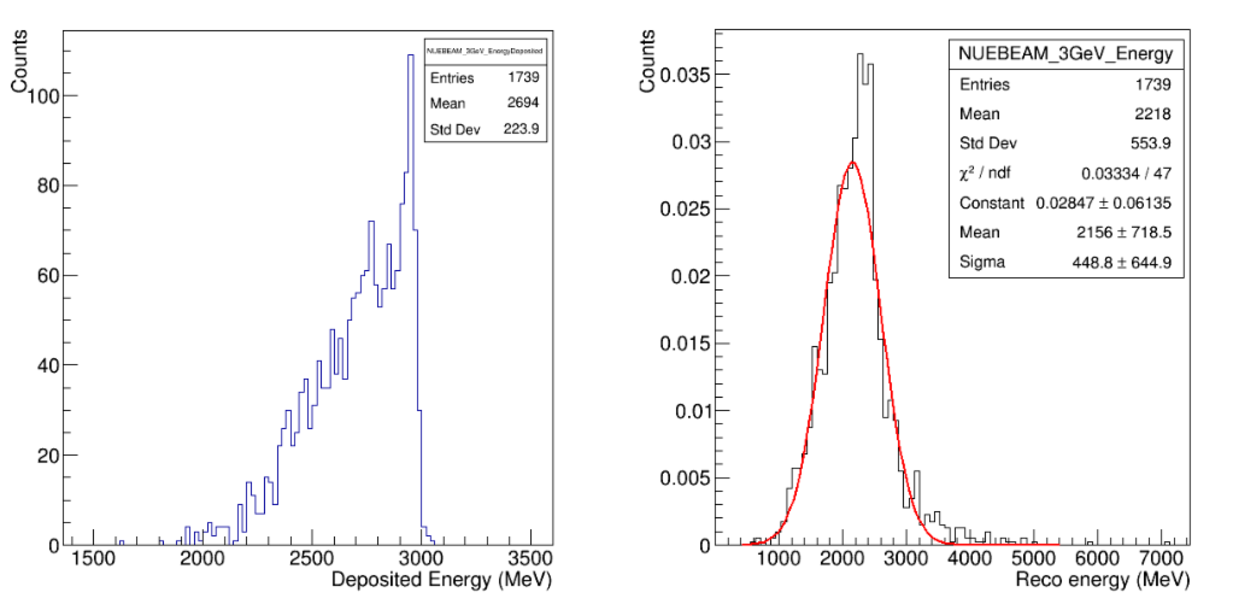
\includegraphics[width=0.95\textwidth]{graphics/dppd_beam_calorimetry.pdf} 
\end{dunefigure}

\begin{dunefigure}[Correlation between \dword{pds}-reconstructed energy and deposited energy for beam neutrino interactions.]{fig:dppd_beam_calorimetry2}
{Correlation between \dword{pds}-reconstructed energy (vertical axis) and true deposited energy in \lar (horizontal axis) for \SI{3}{\GeV} beam \nue \dshort{cc} interactions in the \lar fiducial volume.}
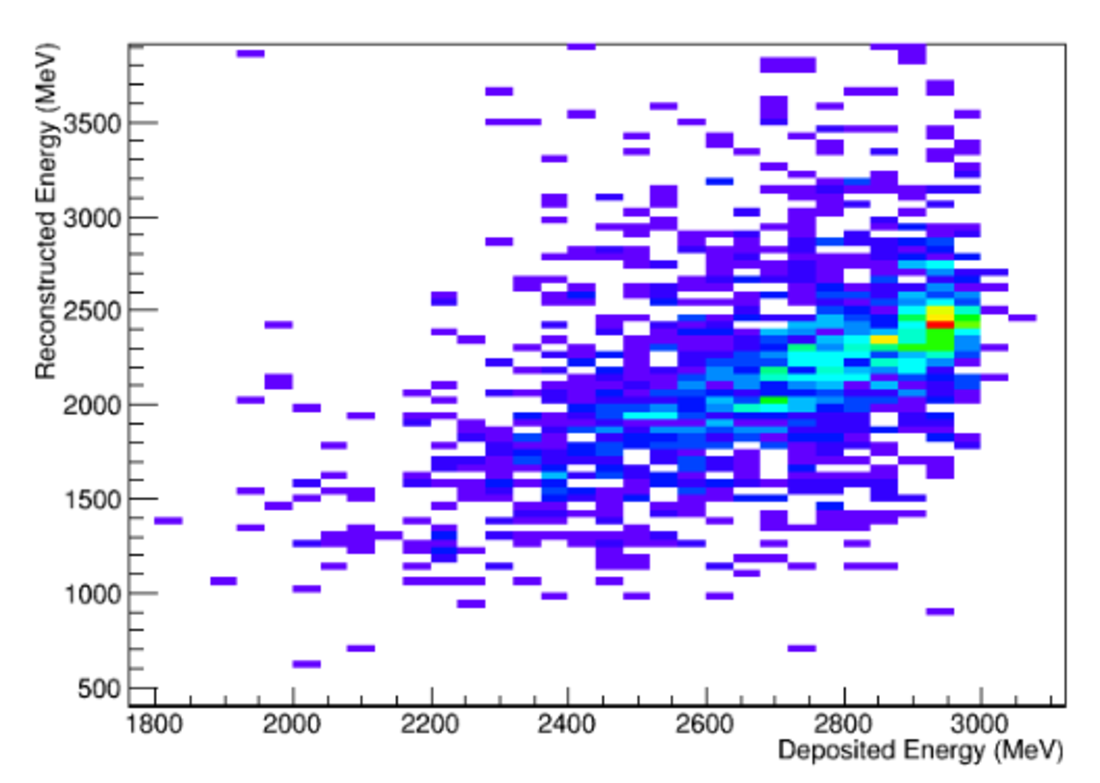
\includegraphics[width=0.60\textwidth]{graphics/dppd_beam_calorimetry2.pdf} 
\end{dunefigure}

We expect to improve the energy resolution performance shown above in two ways:
\begin{description}
   \item[Improved \dword{pds} design:] the results shown above were obtained for the no \dword{wls} foil detector configuration. Studies for the baseline half foil configuration are ongoing. Because of the more uniform response of the baseline design, we expect that the energy resolution will improve.  
   \item[Improved energy reconstruction algorithm:] Eq.~\ref{eq:dppd_ereco} assumes that all the energy is deposited at the neutrino vertex. In practice, events have a certain spatial extent and energy deposition pattern, which the \dword{tpc} can accurately measure. A reconstruction algorithm that accounts for the event extent is expected to perform better, and is under development.
\end{description}
 
\section{Quality Control and Quality Assurance}
\label{sec:dp-pds-quality}

The \dword{qa} and \dword{qc} procedures for the \dual \dword{pds} are based on our experience with the \dword{pddp}. The \dwords{pmt} of the \dual \dword{pds} will go through a series of performance and functionality tests at various locations until commissioning. The mechanical assembly of the \dwords{pmt} will go through mechanical tests, the high voltage cables will be tested for continuity and resistance, the high voltage/signal splitters will be tested for electronics integrity, and the calibration fibers will be tested for high quality transmission. Below  are the details of the quality assurance and control procedures.

\subsection{Quality Control During Production and Assembly}

The \dword{qc} performed at the different institutions, after receiving the \dwords{pmt} from the manufacturer, include \dword{qc} testing before accepting or returning the \dwords{pmt} using established acceptance and rejection criteria. \dword{qc} also includes checking the construction of the base boards, support structures, cables, \dword{hv}/signal splitters, and light calibration units. \dword{qc} also includes mechanical tests of the assembly and performance tests of the \dwords{pmt} and electronics, both at room temperature and when necessary, at cryogenic temperatures. The institutes that perform these tests are referred to as production and assembly sites.

\begin{itemize}
\item The \dwords{pmt} will be visually inspected as they are received from the manufacturer.

\item 
%The baseboards will be tested for electronics integrity as they are produced, before they are connected to the \dwords{pmt}. Once they are connected, mechanical integrity will be tested. 
The \dword{pmt} support structure design is already validated by immersing its mounted \dword{pmt} in cryogenic temperatures and at an over-pressure equivalent to a depth of \SI{12}{m} in \lar{}. Design validation tests are carried out to confirm that the \dword{pmt} base design fulfills the specifications at room and cryogenic temperatures. A cable with a \dword{shv} connector is soldered to each \dword{pmt} base to facilitate the different base and \dword{pmt} tests and the final \dword{pmt} connection during the installation. The \dword{pmt} bases are labeled (on the cable) to track them. After production of the \dword{pmt} base boards, each is individually tested before connecting to the \dwords{pmt} to verify that components are correctly mounted. Later they are cleaned and tested at maximum voltage in an argon gas environment to confirm that no sparks occur. After mounting the bases on the \dwords{pmt}, they are tested again %in argon gas 
at maximum voltage to confirm that no sparks occur due to poor soldering.

\item All the light readout units (\dword{pmt} + base + support) will be tested and characterized in liquid nitrogen to check performance at cryogenic temperature and to obtain a database with the most important parameters for each \dword{pmt} (for example, gain versus voltage, dark counts). The \dword{pmt} base number attached to each \dword{pmt} will also be included in the database.

\item The wrapping materials and techniques are studied with one fully assembled light readout unit. The handling, transportation, and installation scenarios are carefully studied, and the transportation box design is validated. The transport box and \dword{pmt} wrapping must ensure complete darkness.

\item The light output of the \dwords{led} and fiber light transmission from the light calibration system will be measured with a power meter.

\item The high voltage cables will be tested for continuity and for resistance.

\item The high voltage/signal splitters will be tested for electronics integrity followed by  performance tests with a reference \dword{pmt}.

\end{itemize}

%\subsection{Quality Control at the Integration and Testing Facility}
\subsection{Quality Control at the Coating, Testing and Storage Facility}

The \dwords{pmt} will be transported to the \dword{ctsf}, envisaged to be established %in South Dakota 
near the experiment site. As the \dword{pmt} boxes are received, they will be visually inspected to verify they were safely transported. The \dword{tpb} coating of the \dword{pmt} windows will be performed at the \dword{ctsf}. The \dword{pmt} windows will be cleaned before the coating is applied. The \dword{qc} of the cleaning will be qualitative based on experience. The \dwords{pmt} will then be placed in the evaporator, and the coating will be applied. The first few samples will undergo microscopic examination and surface uniformity tests, and the coating procedure will be validated. Subsequent production \dwords{pmt} will be randomly sampled for basic coating \dword{qa}.

Once the coating is finished, the \dwords{pmt} will be packed in special underground transport assembly and placed inside the original transportation boxes. The \dwords{pmt}, however, will not be placed in the cartons. They will have protective covers over the windows. Before being placed in the transportation assembly, the \dwords{pmt} will undergo functionality tests individually. Once all the \dwords{pmt} in a box are validated, the box will be closed and transported to the underground hall.

The \dword{ctsf} is also the primary reception point for the other \dword{dp} \dword{pds} equipment, including cables, fibers, light calibration systems, and \dword{hv}/signal splitters. These boxes will be inspected for verify they were safely transported. Unless signs of  damage to the transportation boxes are obvious, no \dword{qc} inspection will be performed on the individual items. If  damage is identified, the boxes will be opened and visual/functional \dword{qc} tests will be performed. If damaged items can be repaired, that will be done at the \dword{ctsf}. If the damage is not repairable, the items will be returned to the manufacturer or the production/assembly sites.

\subsection{Quality Control at the Underground Areas}

After  transportation from the \dword{ctsf} to \surf, the \dwords{pmt} will be tested for proper functionality in a dedicated light-tight box in the clean room. During installation, the \dword{pmt} database will be updated with the position of each \dword{pmt} (identified by its serial number and base number) in the \dword{detmodule}. After installation, the full connection from the \dword{fe} to the \dwords{pmt} will be checked. The \dword{fe} channel and splitter number connected to each \dword{pmt} will be included in the \dword{pmt} database.

The \dword{hv}/signal cables and the calibration fibers will be transported to the cryostat roof long before the \dwords{pmt} themselves. As they arrive, they will be checked for potential damage during transportation. These tests will include continuity tests for the \dword{hv}/signal cables and qualitative transmission tests for the calibration fibers.

The last step of \dword{qc} will be to test the entire system using the full readout chain (Section~\ref{subsec:dp-pds-commissioning}).

\section{Interfaces}
\label{sec:dp-pds-interfaces}

The \dword{pds} has several interfaces with other subsystems and the global \dword{dune} systems. The interface documents related to \dword{dp} \dword{pds} are given in Table~\ref{tab:dppd_t_8}. Only some of the basic interfaces are summarized below. 

\begin{dunetable}
[\dual \dword{pds} interface documents]
%{|l|c| p{0.8\textwidth}}
{p{0.25\textwidth}p{0.5\textwidth}l}
{tab:dppd_t_8}
{\dual \dword{pds} interface documents.}

%\dual \dword{pd} Interface Document & DUNE docdb number \\ \toprowrule
Interfacing System & Description & Linked Reference \\ \toprowrule
\dword{dp} electronics & Electronics racks, connectors & \citedocdb{6772} \\
\dword{hv} & \dword{fc}, cathode, \dword{gg} and \dword{pds} \dword{pmt} and reflector/\dword{wls} panel assemblies installation sequence, possibility of individual \dwords{gg} on the \dword{pmt} support structures  & \citedocdb{6799} \\
\dword{daq} & Data format, trigger distribution & \citedocdb{6802} \\
%\dword{cisc} & 6781 \\
\dshort{cisc} & Layout of cryogenic instrumentation, slow control of the \dword{pds} power supplies and calibration system & \citedocdb{6781} \\ %capitalize first letter dword workaround
\dune Physics & Physics requirements & \citedocdb{7087} \\
Software and Computing & Development of simulation, reconstruction, and analysis tools & \citedocdb{7114} \\
Calibration & Global monitoring of \dword{pds} \dwords{pmt} & \citedocdb{7060} \\
%\dword{itf} & 7033 \\
%\dword{itf} & Shipping and receiving of the \dword{pds} components, \dword{tpb} coating of the \dwords{pmt} & \citedocdb{7033}\\
Detector and Facilities Infrastructure & \dword{pmt} supporting bases, cable trays, feedthrough flanges, access to conventional facilities, participation in the \dword{ddss} & \citedocdb{6979} \\
\dshort{uit} & Transportation of the \dword{pds} components to and between underground areas, clean room activities, storage, and installation & \citedocdb{7006} \\
\end{dunetable}

%\fixme{Update to standard table format for interface document tables, Sec.~3.5.2 in \url{https://dune.bnl.gov/docs/guidance.pdf}.}

\begin{itemize}

\item \dword{dp} Electronics: The \dword{pds} shares the same \dword{fe} electronics standard as the charge readout, which is \dword{utca}-based \cite{utca}. The \dword{dp} electronics will provide data in continuous streaming %(\num{12} bits at \SI{2.5}{\MHz} sampling) 
of all \dword{pds} channels over the \SI{10}{\Gbps} links. The number of photomultipliers to be read out is \dpnumpmtch, to be distributed among \num{60} AMC cards (\num{20} \dword{utca} crates for the \num{20} \dword{pds} sectors, \num{36} readout channels in \num{3} AMC cards/crate). Readout racks for the sectors will be \SI{6}{\m} apart along the \SI{60}{\m} side and on both sides. Deeper understanding of \dword{pmt} characteristic (e.g., saturation, recovery time, ringing, pre- and after-pulsing) will be provided by \dword{dp} \dword{pds}. The type of connectors used at the FE input panel will be determined by the \dword{dp} Electronics Consortium and will be implemented by \dword{dp} \dword{pds}.

\item \dword{hv}: This interface includes the consideration of the distance between the cathode/ground grid and the \dword{pmt} planes, the installation of the reflector/\dword{wls} panel assemblies on the inner surface of the \dword{fc} and the possible implementation of the ground grid at the individual \dword{pmt} level. The \dword{hv} consortium and \dword{pds} consortium will be communicating to harmonize the underground installation.

\item \dword{daq}: The hardware interface uses mainly optical fibers. \dword{dp} \dword{pds} provides trigger and data in continuous streaming;  the interface also includes the \dword{daq} software.

\item \dshort{cisc}: The main interface points with the \dword{cisc} are the layout of the cryogenic instrumentation (e.g. purity monitors, temperature sensors and light emitting system for the cameras) and the \dword{pmt} support structures and cabling, as well as the slow control of the \dword{pds} power supplies and calibration system. The \dword{pds} \dwords{pmt} are part of \num{20} sectors with \num{36} \dwords{pmt} each and will be controlled with \num{20} \dword{hv} crates.

\item \dune Physics: \dual \dword{pds} has interfaces with the overall physics requirements on energy and time as well as classification of events, decay modes, and neutrino flavors.

\item Software and Computing: This interface involves developing the simulation, reconstruction, and analysis tools.

\item Calibration: The \dword{pds} participates in the \dword{dune} global calibration task force and will provide handles to allow global monitoring of \dword{pmt} performance.

%\item \dword{itf}: The operations at the \dword{itf} are described in Section~\ref{subsec:dp-pds-itf}. The interface items can be summarized as shipping and receiving of the \dword{pds} components, \dword{tpb} coating of the \dword{pmt} windows, basic functionality testing, repairing, and repackaging at the facility. The interface includes recycling and returning packaging materials.

\item Detector and Facilities (\dword{lbnf}) Infrastructure: The \dword{pds}
\dword{pmt} supporting base on the cryostat floor; cold cables and cable trays; and the feedthroughs are the major interfaces with the facility. The cable trays from the ceiling \fdth flanges to the bottom of the cryostat in which the cables and calibration fibers are routed fall under the responsibility of the facility. Installing the \dwords{pmt} and connecting the fibers and \dword{hv}/signal cables to the \dwords{pmt} fall under the responsibility of \dword{pds}. Other interfaces with the facility include access to conventional facilities and participation in the \dword{ddss}.

\item \dshort{uit}: This interface with the \dword{uit} includes the transportation of \dword{pds} components to and between underground areas, clean room activities, storage, and coordination of the installation with the other teams. The details are described in Section~\ref{subsec:dp-pds-undergroundinstallation}.

\end{itemize}


\section{Installation, Integration, and Commissioning}
\label{sec:dp-pds-installation}

\subsection{Transport and Handling}

\dwords{pmt} will be transported on a standard EUR pallet that is \SI{1.2}{\m} $\times$ \SI{1}{\m}. Figure~\ref{fig:dppd_11_2} shows the largest capacity commercially available box. The box can hold \num{36} \dwords{pmt} in three levels of \num{4} $\times$ \num{3} arrays. Individual \dwords{pmt} will be placed in cartons with their bases, support structures, and short \dword{hv} cables soldered to the bases at the production/assembly sites. For shipping to \dword{ctsf}, \num{36} \dwords{pmt} will then be placed in the transport boxes.

\begin{dunefigure}[An example transportation box to be used for all transport purposes i.e. from remote sites to the \dword{ctsf} and from \dword{ctsf} to \surf.]{fig:dppd_11_2}
{An example transportation box to be used to transport items from remote sites to the \dword{ctsf} and from \dword{ctsf} to \surf.}
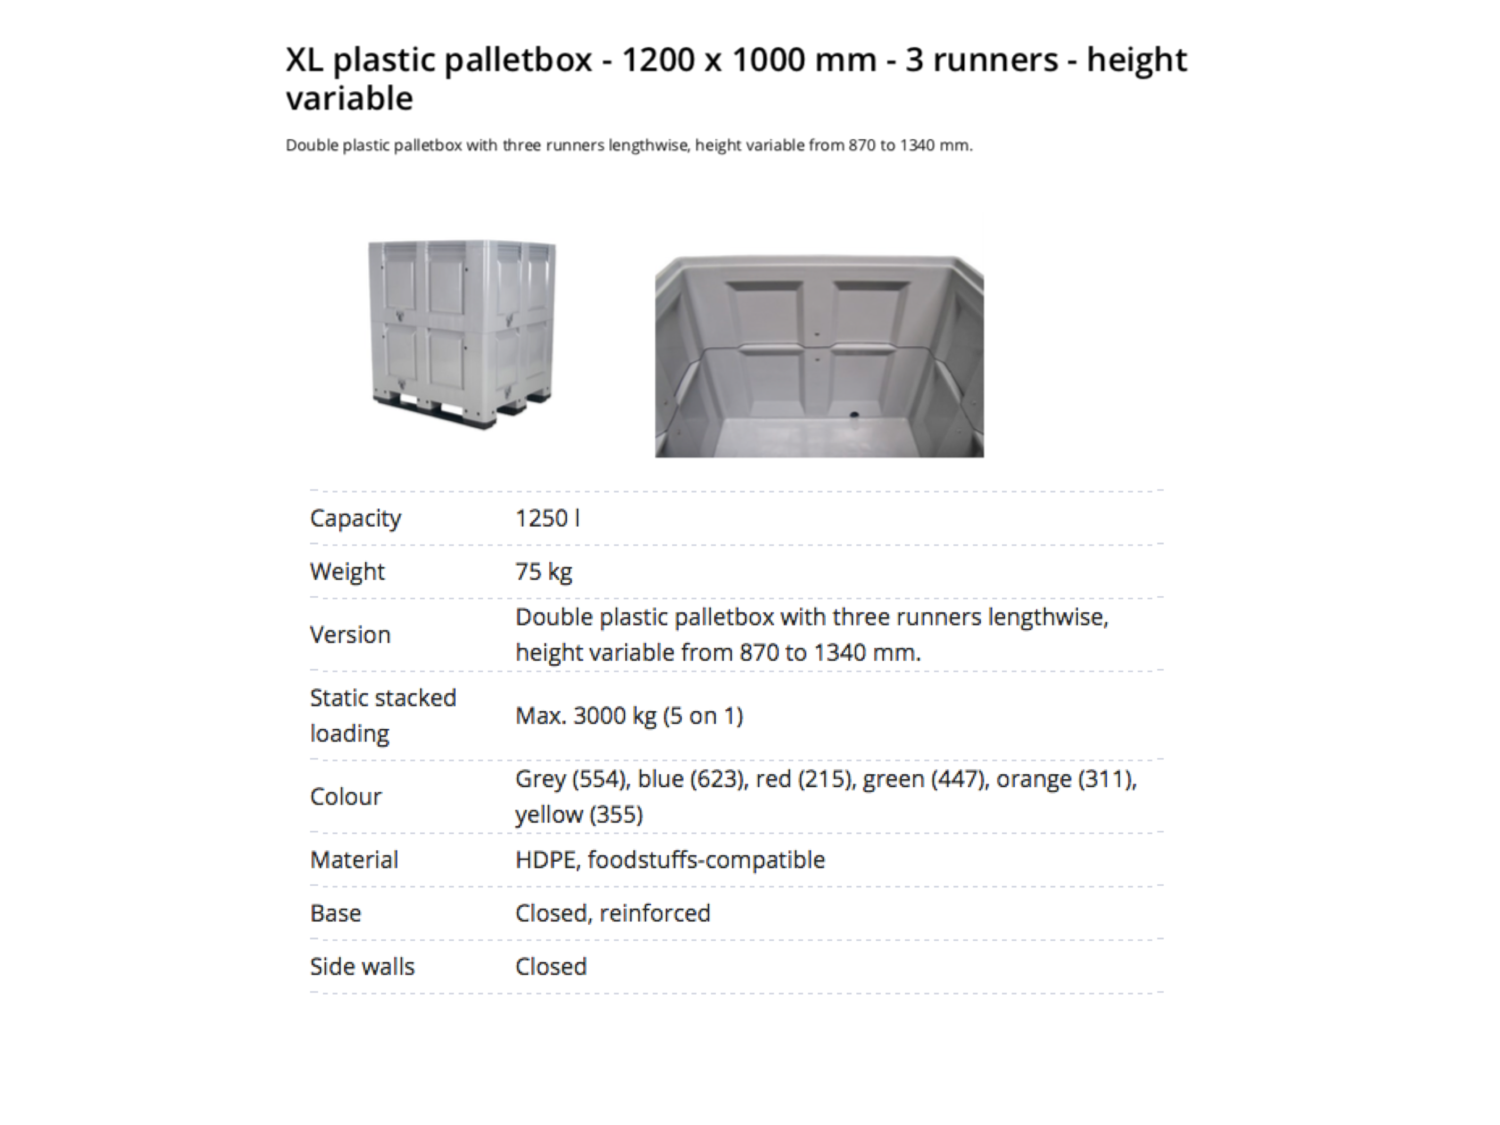
\includegraphics[width=0.5\textwidth]{dppd_11_2}
\end{dunefigure}

Following the \dword{ctsf} operations, the \dwords{pmt} will be placed in a custom structure in \num{4} $\times$ \num{3} arrays. The structure will be assembled with metal and plastic parts so the entire structure, together with the \dwords{pmt}, can be moved into the clean room underground. Three of these structures will be placed on top of each other inside the boxes with the crane. The individual cartons that held the \dwords{pmt} will be recycled at the \dword{ctsf}. The local movement of the transportation boxes in the \dword{ctsf} can be done with compact warehouse forklifts. The \dword{ctsf} will also be used as the storage area for the large \dword{pmt} transportation boxes before they are sent to \surf. The boxes will be stored in single-shelf racks to the right and left of the entrance to the work area (Fig.~\ref{fig:dppd_11_3}). The first set of boxes will be placed on the floor and the second set will be on a shelf that is \SI{1.5}{\m} off the ground. This area can store the entire \dual \dword{pds} \dword{pmt} inventory of \dpnumpmtch \dwords{pmt} in \num{20} boxes. The \num{80} spare \dwords{pmt} can be placed in three boxes, which can be stored on the floor in the available space in the work area as the \dual \dword{pds} \dword{ctsf} operations are finished.

The large \dword{pds} boxes will be wrapped with plastic foil at the \dword{ctsf} that will be opened in \dwords{sas} underground. After removing the plastic wrapping, the transport boxes, with their entire contents, will be moved into the cleanroom. The \dword{pds} boxes can be moved around the underground areas with a pallet jack. Each \num{4} $\times$ \num{3} structure will be removed from the transportation box and moved inside the cleanroom by the crane. The structure will go in the dark box for functionality tests of the \num{12} \dwords{pmt}. The transportation boxes will be used for storage before installation. Empty boxes will be returned to \dword{ctsf}. At most, three \dword{pds} boxes will be in the cleanroom at a time.

The \num{4} $\times$ \num{3} structure will be moved by crane into the cryostat and placed on the cryostat floor at a location convenient to the active installation area. The \dwords{pmt} will then be installed one by one. 

%\subsection{Integration and Testing Facility Operations}
\subsection{Coating, Testing and Storage Facility Operations}
\label{subsec:dp-pds-itf}

The \dword{ctsf} will be \SI{10}{\m} $\times$ \SI{8}{\m} with a (\SI{12}{\ft}) ceiling equipped with a gantry crane. The facility will be used to apply the \dword{tpb} coating on the \dword{pmt} windows, for \dword{qc} of the \dwords{pmt}, and for storage and preparation for transport to \surf. If the option of installing individual ground grids on the \dword{pmt} support structures, which is under consideration by the \dual \dword{pds} and \dword{hv} consortia, is realized, this operation will also be performed at the \dword{ctsf}. The layout of the \dword{ctsf} is shown in Figure~\ref{fig:dppd_11_3}.

\begin{dunefigure}[The layout of the \dword{ctsf}.]{fig:dppd_11_3}
{The layout of the \dword{ctsf}.}
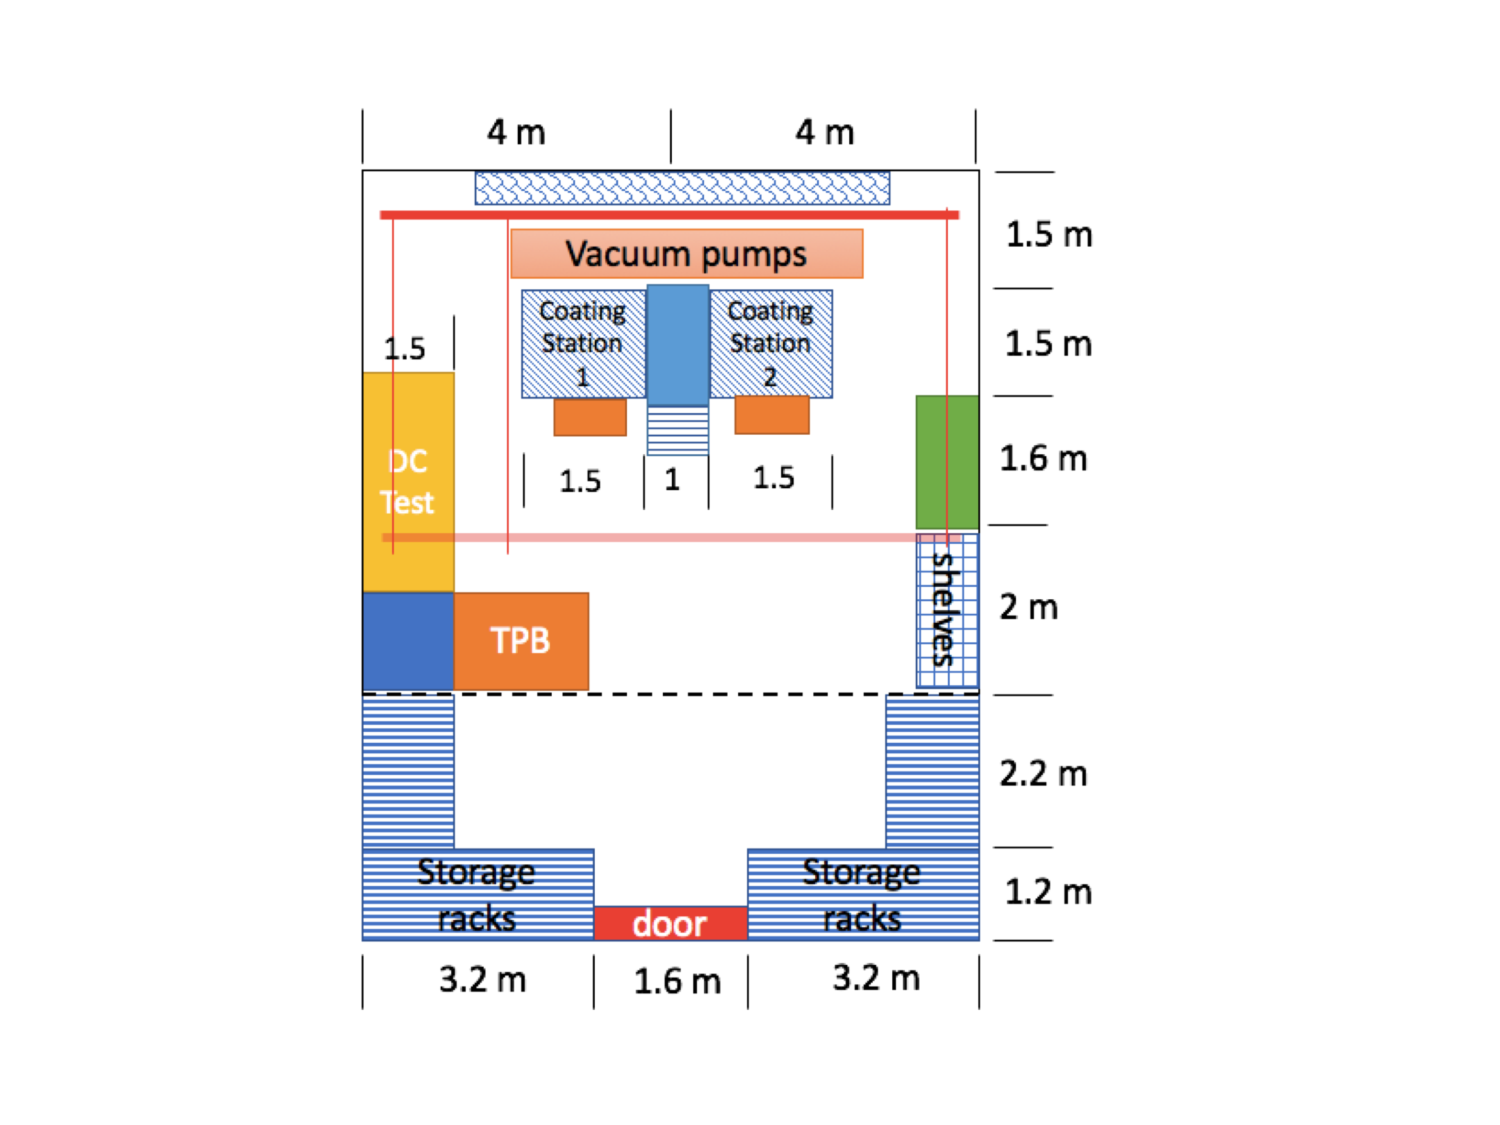
\includegraphics[width=0.4\textwidth]{dppd_11_3}
\end{dunefigure}

Two coating stations will be \SI{1.5}{\m} $\times$ \SI{1.5}{\m}. Figure ~\ref{fig:dppd_11_4} shows pictures of a \dword{tpb} coating station at the \dword{cern} thin film facility. Between the two coating stations, an elevated platform, accessible by stairs, will be placed. This platform will be used to reach the top of the evaporator (approximately \SI{1.5}{\m} high from the ground level) and inside the vessel. Cooling water, nitrogen, and electricity will be provided from the outlets placed along the \SI{8}{\m} wall (indicated with wavy lines in Figure~\ref{fig:dppd_11_3}). Vacuum pumps will be placed in the immediate vicinity of the evaporators. Control electronics will also be placed next to the evaporator chambers. 

\begin{dunefigure}[Pictures of a single \dword{tpb} coating station (courtesy of Wil Vollenberg, \dword{cern}-TE Department).]{fig:dppd_11_4}
{Pictures of a single \dword{tpb} coating station (courtesy of Wil Vollenberg, \dword{cern}-TE Department).}
\includegraphics[width=0.8\textwidth]{dppd_11_4}
\end{dunefigure}

The \dwords{pmt} will be taken out of their individual cartons when they arrive at the \dword{ctsf}. The \dwords{pmt} will first be tested for basic functionality in their cartons to verify that they have been safely transported from the remote sites and will be kept in these boxes until the windows are coated. The \dword{pmt} windows will be cleaned with acetone and isopropanol before the evaporation. This will be done in the flow device/fume hood shown as a green box along the \SI{10}{\m} wall in Fig.~\ref{fig:dppd_11_3}. The gantry crane (indicated with red bars in Fig.~\ref{fig:dppd_11_3}) can move parts between the coating stations and the work desks. It will be used to remove the vessel lid and support it while the \dword{pmt} is installed for coating.

Following the evaporation procedure, an acrylic protective plates will be installed to cover the coated \dword{pmt} windows.
%, and the \dwords{pmt} will be placed in individual dark plastic protective bags. 
The \dwords{pmt} will be tested again for basic functionality. They will then be attached to the \num{4} $\times$ \num{3} structure for transportation to \surf.

At the \dword{ctsf}, the \dword{pmt} windows will be coated at a rate of \num{4} \dwords{pmt}/day or \num{20} \dwords{pmt}/week and \num{80} \dwords{pmt}/month. Given the installation rate of \num{120} \dwords{pmt}/month, the \dword{ctsf} operations should start before installation begins. \dword{ctsf} has sufficient storage capacity for the entire \dword{pmt} inventory of the \dword{pds}. 

\subsection{Underground Installation and Integration}
\label{subsec:dp-pds-undergroundinstallation}

The cryostat cable/fiber installation will precede the installation of the \dword{fc}. The cables/fibers will be routed from the flanges to the bottom of the cryostat. The total cable/fiber mass (length) is approximately \SI{50}{\kg} (\SI{25}{\m}) per sector with an average mass/length of \SI{2}{\kg/\m}, where one sector comprises \num{36} \dwords{pmt} (see Section~\ref{sec:dp-pds-overview_layout}). The free ends of the cables/fibers will be temporarily attached to the cryostat floor so they can be easily accessed during installation. The cable/fiber and tray installation will be done on both sides of the cryostat. At this stage, the \dword{hv} cables will be transported in a single box from the \dword{ctsf} to \surf. At the same time, a separate box containing \num{120} calibration fiber + fiber bundle assemblies will be transported from the \dword{ctsf} to \surf. The boxes will be transported to the cryostat roof so the cables/fibers can be hung through the feedthroughs for installation in the cable trays.  

Once the plastic wrap is removed, the \dword{pds} \dword{pmt} box and its entire contents can be moved to the clean room. The \dwords{pmt} will undergo functionality tests inside the custom design dark box, which can cover the entire structure of \num{4} $\times$ \num{3} \dwords{pmt}. The dark box will have a high voltage patch panel and allow consecutive tests of all \num{12} \dwords{pmt} in one testing session without intervention. The test will be a simple check for healthy \dword{pmt} operations. Once the operation of the \dwords{pmt} is verified, the structure can be moved into the cryostat.

Inside the cryostat, the \dwords{pmt} will be removed from the structure. %The window protections will be kept on the \dwords{pmt}. 
The \dwords{pmt} will be mounted on the membrane floor in the areas between the membrane corrugations using their support structures. The attachment is done using a stainless steel support base that can be point-glued to the membrane. The weight of the support and the \dword{pmt} exceeds the buoyancy force of the system. Furthermore, these supports also ensure stability against possible lateral forces acting on the \dwords{pmt} due to the liquid flow. Once the attachment is complete, the short \dword{hv} cables will be connected to the cold \dword{hv} cables with SHV barrel connectors. The calibration fibers will be routed and connected to the support structure. Once all the \dwords{pmt} of a given \dword{pds} sector are installed, the cables and fibers will be fixed in their final positions.

The installation will be done at a rate of \num{30} \dwords{pmt}/week. After installation, the empty \dword{pmt} boxes and the transport structures will be taken back to \dword{ctsf}.

Table~\ref{tab:dppd_t_11_1} summarizes the quantities related to the \dual \dword{pds} installation.

\begin{dunetable}
[Quantities related to the \dual \dword{pds} installation.]
{lc p{0.8\textwidth}}
{tab:dppd_t_11_1}
{Quantities related to the \dual \dword{pds} installation.}
Parameter & Value \\
Number of \dual \dword{pds} sectors	& \num{20} \\
Number of \dwords{pmt} per sector	& \num{36} \\
Number of calibration fibers per sector	& \num{6} \\
Number of feedthrough flanges per sector	& \num{1} \\
Total number of feedthrough flanges	& \num{20} \\
Number of \dword{hv} racks per sector	& \num{1} \\
Frequency of transportations to \surf from \dword{ctsf}	& \num{4} \dword{pds} boxes per month \\
Rate of installation	& \num{30} \dwords{pmt}/week \\
\end{dunetable}

The reflector/\dword{wls} panels will be assembled into a unit panel assembly on a dedicated table underground immediately prior to the installation following the procedure described in Section \ref{sec:dp-pds-mechanics}. They will be placed in a storage structure that can hold three regular and two extended reflector/\dword{wls} panel assemblies to be installed in one row of an \dword{fc} super-module. The installation of the panel assemblies will be synchronized with the installation of the \dword{fc} modules, which is described in Section \ref{sec:fddp-hv-transport-install} and depicted in Fig. ~\ref{fig:dp-super-module-installation-secuence}. Once a row of the \dword{fc} super-module is installed, the five reflector/\dword{wls} panel assemblies will be mounted on the FRP I-beams of the \dword{fc} submodules, starting from one end of the row and progressing towards the other. Figure \ref{fig:dppd_reflective_panel_installation_sequence} depicts the installation sequence of a unit reflector/\dword{wls} panel. The sequence can be described as below:

\begin{enumerate}
\item Put the top two screws accessing the back side through the top liquid flow opening (Fig.~ \ref{fig:dppd_reflective_panel_installation_sequence}  left).
\item Place two nuts in the closed holes of the long holding bar. Slide the long bar behind the panel to the level of the middle bar by holding it through the central liquid flow opening. Put the two middle bar screws and remove the long bar through the bottom liquid flow opening after sliding it all the way down (Fig.~ \ref{fig:dppd_reflective_panel_installation_sequence}  center).
\item Put the bottom two screws accessing the back side through the bottom liquid flow opening (Fig.~ \ref{fig:dppd_reflective_panel_installation_sequence}  right).
\end{enumerate}

\begin{dunefigure}[The schematic view of the installation sequence of a unit reflector/\dword{wls} panel assembly on the \dword{fc} I-beams.]{fig:dppd_reflective_panel_installation_sequence}
{The schematic view of the installation sequence of a unit reflector/\dword{wls} panel assembly on the \dword{fc} I-beams.}
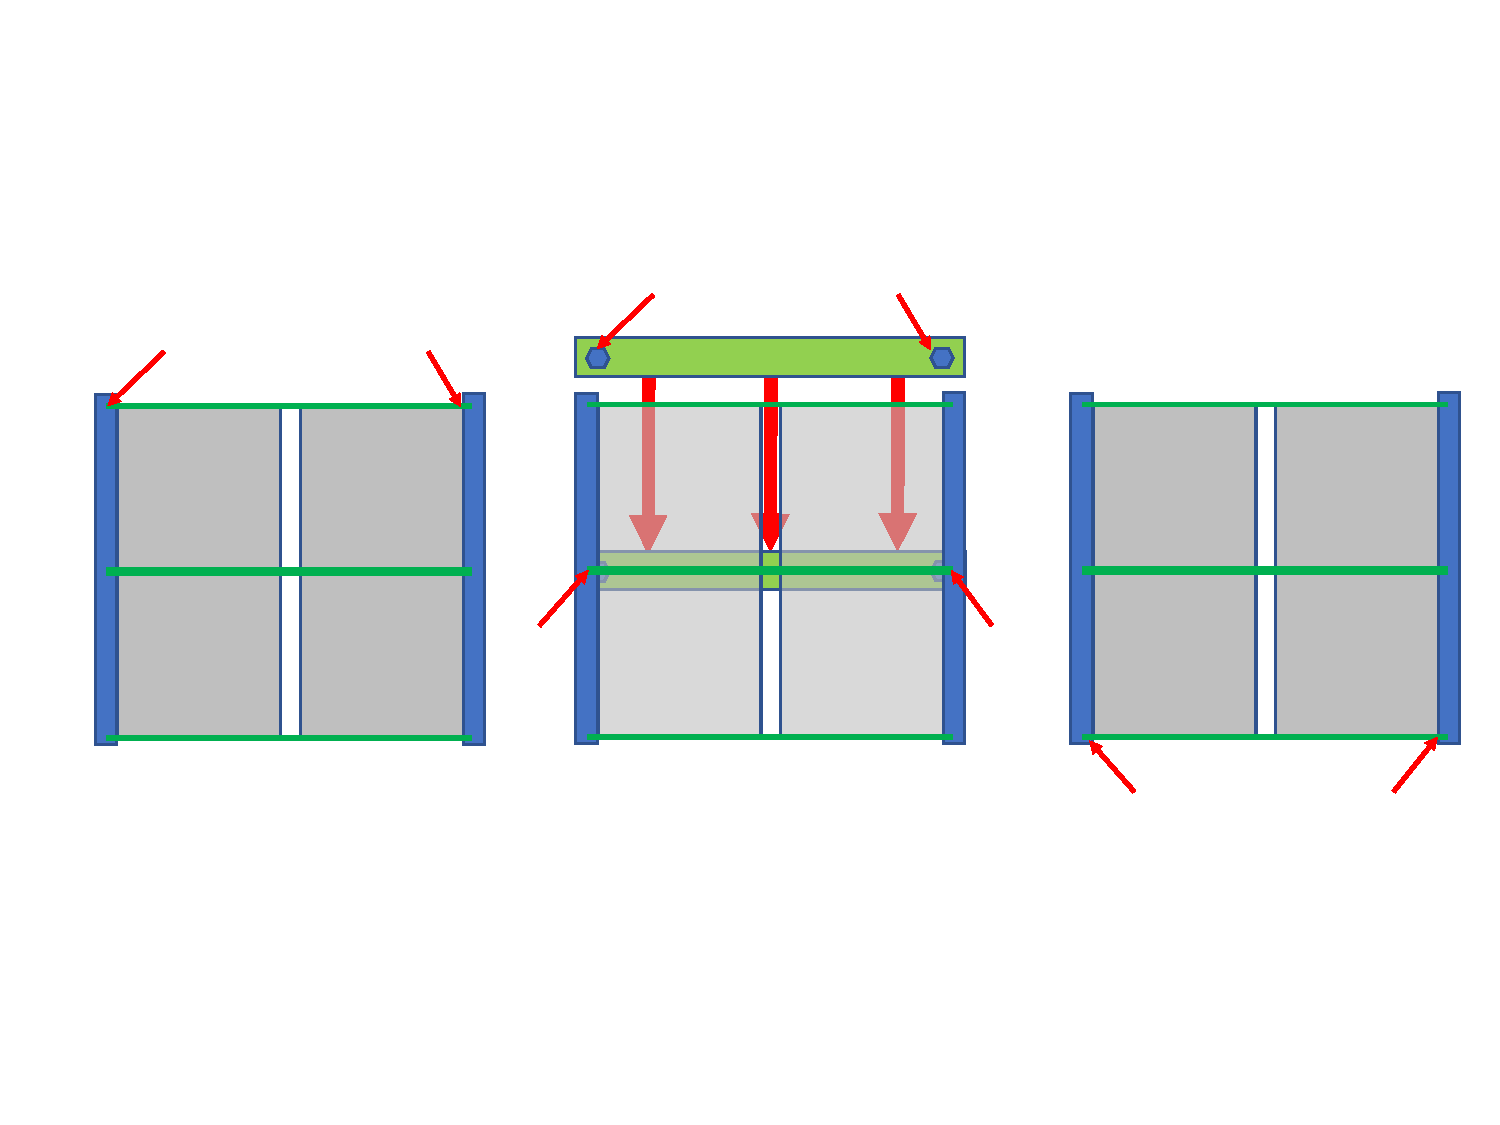
\includegraphics[width=0.8\textwidth]{dppd_reflective_panel_installation_sequence}
\end{dunefigure}

\subsection{Commissioning}
\label{subsec:dp-pds-commissioning}

The commissioning of the \dword{pds} is performed in partitions. The size of a single partition will be mainly determined by the \dword{daq} and the \dword{hv} systems. The \dword{daq} and \dword{hv} partitions are commissioned, including the relevant control systems, before the \dwords{pmt} are connected to these systems.

The exact availability of the cryostat as a sufficiently dark environment depends on the overall installation schedule. Once it is possible, the \dwords{pmt} are powered up, and basic functionality and performance checks are carried out. These include pedestal data taking, i.e., recording event data with external periodic triggering, and tests with the calibration system where the data taking is triggered in synchronization with a light source, as described in Section \ref{sec:dp-pds-calibration}.

Basic performance characteristics of the \dwords{pmt}, e.g., the dark count rate and gain, will be validated with the commissioning tests. Issues related to installation can then be identified and eliminated. A commissioned sector becomes a part of the overall detector and can join the global calibration data taking and commissioning.



\section{Risks}
\label{sec:dp-pds-risks}

Table \ref{tab:risks:DP-FD-PDS} summarizes the risks associated with the \dual \dword{pds}. Severity level assigned for each risk is indicated as L (low), M (medium), and H (high). Severity levels are split into three columns: probability for a risk to occur (P), and impact in terms of cost (C) and schedule (S) that the materialization of a risk would have. Below, we discuss these risks and mitigation plans for each risk item.


% risk table values for subsystem SP-FD-PDS
\begin{longtable}{p{0.18\textwidth}p{0.20\textwidth}p{0.32\textwidth}p{0.02\textwidth}p{0.02\textwidth}p{0.02\textwidth}} 
\caption{Risks for DP-FD-PDS \fixmehl{ref \texttt{tab:risks:DP-FD-PDS}}} \\
\rowcolor{dunesky}
ID & Risk & Mitigation & P & C & S  \\  \colhline
RT-DP-PDS-001 & Insufficient light yield due to inefficient \dword{pds} design & Increase \dword{pmt} photo-cathode coverage and/or \dword{wls} reflector foils coverage. & L & M & L \\  \colhline
RT-DP-PDS-002 & Poor coating quality for \dword{tpb} coated surfaces and \dword{lar} contamination by \dword{tpb} & Test quality and ageing properties of \dword{tpb} coating techniques. Elaborate improved techniques if needed. & M & L & L \\  \colhline
RT-DP-PDS-003 & \dword{pmt} channel loss due to faulty \dword{pmt} base design & Improve \dword{pmt} base design from analysis of possible failure modes in \dword{pddp}. Optimize clustering algorithms to mitigate possible chanel loss. & L & L & L \\  \colhline
RT-DP-PDS-004 & Bad \dword{pmt} channel due to faulty connection between \dword{hv}/signal cable and \dword{pmt} base & Enhcanced connectivity tests in \lntwo prior to installation. Optimize clustering algorithms to mitigate possible chanel loss. & L & L & L \\  \colhline
RT-DP-PDS-005 & Incorrect choice of feedthroughs for the cabling and installation in the cryostat & Improve feedthrough design in case unsatisfactory noise levels during \dword{pddp} operations are present. & L & L & L \\  \colhline
RT-DP-PDS-006 & \dword{pmt} signal saturation & Tuning of \dword{pmt} gains. In the worst case, redesign front-end electronics to adjust the analog input range of ADC. & M & L & L \\  \colhline
RT-DP-PDS-007 & Excessive electronics noise to distinguish \dword{lar} scintillation light & Measurement of noise levels during commissioning prior to \lar filling. Modifications to grounding, shielding, or power distribution schemes. & M & L & L \\  \colhline
RT-DP-PDS-008 & Availability of resources for work at the installation/integration site less than planned & Move expert personnel temporarily from institutions involved in the \dword{pds}consortium to the integration/installation site. & M & L & L \\  \colhline
RT-DP-PDS-009 & Damage of \dwords{pmt} during shipment to the experiment site & Special packaging to avoid possible \dword{pmt} damage during shipment. Contingency of \num{ 10}\% spare \dwords{pmt}. & L & L & L \\  \colhline
RT-DP-PDS-010 & Damage of optical fibers during installation & Fibers will be the last \dual \dword{pds} item to be installed. Detailed documentation for all \dual \dword{pds} installation tasks.   & L & L & L \\  \colhline
RT-DP-PDS-011 & Excessive exposure to ambient light of \dword{tpb} coated surfaces, resulting in degraded performance & \dword{tpb} coated surfaces temporarily covered until cryostat closing. Detailed installation procedure to minimize exposure to ambient light. & L & L & L \\  \colhline
RT-DP-PDS-012 & \dword{pmt} implosion during \dword{lar} filling & No mitigation necessary, considering \SI{7}{bar} pressure rating of \dwords{pmt} and experience with same/similar \dwords{pmt} in other large liquid detectors. & L & L & L \\  \colhline
RT-DP-PDS-013 & Insufficient light yield due to poor \dword{lar} purity & Procurement of \dword{lar} from the manufacturer will require less than \SI{3}{ppm} in nitrogen. & M & L & L \\  \colhline
RT-DP-PDS-014 & \dword{pmt} channel or \dword{pds} sector loss due to failures in \dword{hv}/signal rack & Ease of maintenance outside cryostat and availability of spares for all components of at least one \dword{hv}/signal rack. & L & L & L \\  \colhline
RT-DP-PDS-015 & Unstable response of the photon detection system over the lifetime of the experiment & Channel-level instabilities corrected via light calibration system. Detector-level instabilities corrected via cosmic-ray muon calibration data. & L & L & L \\  \colhline

\label{tab:risks:DP-FD-PDS}
\end{longtable}

%%%%%%%%%%%%%%%%%%%%%%%%%%%%%%%%%%%%%%%%%%%%%%%%%%%%%%%%%%%%%%%%%%%%

\subsection{Design and Construction Risks}
\label{sec:dp-pds-risks_design}

\begin{itemize}

\item Because of the long drift distance and the position of the cathode and ground grid on top of the \dwords{pmt}, the number of photons detected by the \dwords{pmt} might not be sufficient at some geometrical acceptances (RT-DP-PDS-001). This is estimated as low-probability risk, given that the current \dword{pds} design has been optimized based on detailed simulations. The \dword{pds} baseline design includes \dword{wls} reflector foils precisely to address the risk of insufficient light levels, see Sec.~\ref{sec:dp-pds-simulation}. The detailed understanding of the light levels observed in the \dword{wa105} and particularly in \dword{pddp} will further mitigate this risk. The \dune \dword{fd} \dword{pds} design is essentially a large-scale replica of the recently installed \dword{pddp} \dword{pds}. The most notable exception is the \dword{wls} reflector foils, that is considered to be tested in a \dword{pddp} \dword{pds} upgrade. The largest variation in light yield occurs along the drift direction, where the extrapolation from \dword{pddp} size to the \dune \dword{fd} module size is only a factor of two. If higher \dword{pds} detection efficiency turns out to be necessary, the number of \dwords{pmt} may be increased and/or the surface area of \dword{wls} reflector foils may be increased.

\item Past experience shows that the \dword{tpb} coating might not be sufficiently stable (RT-DP-PDS-002). \dword{tpb} emanation from coated surfaces (\dword{pmt} photo-cathodes and \dword{wls} reflector foils) into the bulk \dword{lar} may cause \dword{wls} behaviour of the contaminated \dword{lar} bulk, or create a loss in optical performance of the coatings over time. This is estimated as medium-probability risk. Certain coating techniques have shown to emanate \dword{tpb} up to tens of parts per billion into argon by mass \cite{Asaadi:2018ixs}, although such impurity levels are not expected to be problematic. In addition, other \dword{lar} experiments using \dword{tpb} coatings, most notably DarkSide-50 \cite{Agnes:2018fwg} and DEAP-3600 \cite{Ajaj:2019imk}, have already shown percent-level stability in \dword{pds} light yields over timescales of 1--2 years. Nevertheless, different coating techniques vary greatly in terms of coating quality and stability. As risk mitigation measure, we plan to test the quality and ageing properties of the exact coating procedure to be followed for the \dword{pmt} photo-cathodes and \dword{wls} reflector foils in \dword{pddp} and in dedicated R\&D setups. We will elaborate improved coating techniques if needed.

\item An inadequate \dword{pmt} base design may result in dead \dword{pmt} channels during the long lifetime of the experiment (RT-DP-PDS-003). Such channel losses could not be recovered. This risk is estimated as low-probability. On the one hand, the loss of single \dword{pmt} channels is expected to have a minimal impact on detector performance. Current \dword{pmt} clustering algorithms (see Sec.~\ref{sec:dp-pds-performance}) already allow for non-responsive \dwords{pmt} along one row or column within one optical cluster. On the other hand, the \dword{pmt} base design is a mature and simple design already tested in the \dword{wa105} and to be tested in \dword{pddp}. \dword{pddp} operations will provide additional risk mitigation. If \dword{pddp} experience with \dword{pmt} bases proves to be unsatisfactory, design modifications will be introduced and tested.

\item \dword{pmt} cables are soldered to the \dword{pmt} base and tested before installation. If the soldering is poorly done, some channels could show a bad waveform or no signal at all (RT-DP-PDS-004). Such noisy or dead channels could not be repaired. This risk is estimated as low-probability. On the one hand, and as discussed above, the loss of single \dword{pmt} channels is expected to have a minimal impact on detector performance. On the other hand, the \dword{pmt} with final base plus soldered cable will be tested in \lntwo during the \dword{pmt} characterization tests, see Sec.~\ref{sec:dp-pds-selection-characterization}. In addition, several tests will be done in the base before the \dwords{pmt} are installed: impedance, \dword{hv} tests in gas Ar to avoid sparks, and full test of the \dword{pmt} to verify signals are correct.

\item Choosing the wrong feedthrough means we could have higher noise levels or oscillations in the signals (RT-DP-PDS-005). Using the wrong parts might cause mechanical problems. Special care must be taken during the design of the screws and \dword{hv} feedthroughs needed for cabling in the detector. \dword{pddp} experience will be used to mitigate this risk, estimated to be low-probability.

\item \dword{pmt} signal saturation at the front-end input (RT-DP-PDS-006) may occur as a result of operation at a higher-than-anticipated \dword{pmt} gain, for example to compensate for a poor signal-to-noise ratio. \dword{pmt} signals may also saturate because of an incorrect signal amplitude estimate. This risk is estimated to be medium-probability, also considering the highly non-uniform \dword{pds} spatial response. \dword{pmt} signal saturation would have minimal impact on \dword{pds} $t_0$ reconstruction and triggering capabilities. It would have more impact on \dword{pds} energy reconstruction capabilities, although some amount of saturation can be tolerated also in this case (see Sec.~\ref{sec:dp-pds-performance}). To mitigate this risk, we will avoid operating the \dwords{pmt} at very high voltages. A balance between gain and saturation will be chosen.

\item Excessive noise on \dword{pmt} waveforms could appear because of poor grounding design, insufficient cable shielding or noisy power distribution (RT-DP-PDS-007). The risk is estimated as medium-probability. This problem could be detected during \dword{pds} commissioning. Doing so prior to \dword{lar} filling is essential, in case necessary modifications to grounding, shielding, or power distribution  schemes affect components inside the cryostat.

\end{itemize}

%%%%%%%%%%%%%%%%%%%%%%%%%%%%%%%%%%%%%%%%%%%%%%%%%%%%%%%%%%%%%%%%%%%%

\subsection{Risks During Installation}
\label{sec:dp-pds-risks_installation}

\begin{itemize}

\item Availability of resources for work at the installation/integration site may be less than planned (RT-DP-PDS-008). This risk is estimated to be medium-probability. The \dword{fd} construction cost estimate assumes that qualified local labor can be identified for certain activities.  The cost will increase if external labor is required.  Labor costs might need to increase to attract qualified candidates. Labor resources from laboratories may need to be housed and used. We will ensure that sufficient funding is available to move people temporarily from institutions involved in the \dword{pds} consortium to the integration/installation site.

\item If \dwords{pmt} are not packaged properly, they could be damaged during shipment (RT-DP-PDS-009). In this case, the \dword{pmt} cannot be used in the detector. This risk is estimated to be low-probability. We will use special packaging to avoid possible damage to the \dwords{pmt} during shipment. In any case, we will have a \num{10}\% contingency spare \dwords{pmt}.

\item Fibers are fragile and could be broken during installation because of the high number of fibers in the detector (RT-DP-PDS-010). This risk is estimated to be low-probability. Personnel in charge of assembling the different parts of the detector must take special care during fiber installation.

\item \dword{tpb} coated surfaces (\dword{pmt} photo-cathodes and \dword{wls} reflector foils) are sensitive to ultraviolet light exposure, which may cause degraded optical performance (RT-DP-PDS-011), see for example \cite{Jones:2012hm}. This risk is estimated to be low-probability. \dword{tpb} coated surfaces will be covered with plastic bags or filters to avoid photo-degradation until closing of the cryostat. The installation procedure for \dwords{pmt} and \dword{wls} reflector foils will be defined in great detail, to minimize exposure to ambient light. 

\end{itemize}

%%%%%%%%%%%%%%%%%%%%%%%%%%%%%%%%%%%%%%%%%%%%%%%%%%%%%%%%%%%%%%%%%%%%

\subsection{Risks During Commissioning}
\label{sec:dp-pds-risks_commissioning}

\begin{itemize}

\item Filling the detector with \dword{lar} could become a critical issue in the occurrence of a \dword{pmt} implosion (RT-DP-PDS-012). If this happens, a chain reaction may develop, as in the Super-Kamkionande detector accident of 2001, destroying several other \dwords{pmt}. If a \dword{pmt} implosion occurs, the detector must be emptied, and the \dwords{pmt} would have to be reinforced or removed. This risk is estimated to be low-probability. The Hamamatsu R5912 \dwords{pmt} are rated for \SI{7}{bar} pressure and the hydrostatic pressure on the cryostat floor will be about \SI{2}{bar}. Similar 8-inch tubes, with same pressure rating, have been successfully used in other large detectors, such as MiniBooNE, SNO, ICARUS T600 and DEAP-3600, and in similar pressure conditions. In addition, a computational model to calculate the shock wave pressure resulting from tube implosion was developed for the MiniBooNE experiment, based upon the stored energy in an evacuated tube at a given depth \cite{Brice:2006ny}. It should be noted that the energy stored in an \SI{8}{inch} \dword{pmt} is over an order of magnitude less than in a \SI{20}{inch} Super-K \dword{pmt}. That study indicated a large safety factor against a chain reaction of \dword{pmt} implosions, and for the more densely packed MiniBooNE \dwords{pmt}.

\end{itemize}

%%%%%%%%%%%%%%%%%%%%%%%%%%%%%%%%%%%%%%%%%%%%%%%%%%%%%%%%%%%%%%%%%%%

\subsection{Risks During Operation}
\label{sec:dp-pds-risks_operation}

\begin{itemize}

\item A high level of \dword{lar} contamination may result in an unacceptably short absorption length for argon scintillation light, thus in an unacceptably low detected light yield despite a satisfactory \dword{pds} design (RT-DP-PDS-013). This risk is estimated as medium-probability. A particularly harmful contaminant, as far as light detection is concerned, is nitrogen. The simulation studies presented in this chapter assume an argon scintillation light absorption length of \SI{20}{m}, corresponding to about \SI{3}{ppm} of N$_2$ impurity concentration. Such argon purity specification has already been achieved in large \dword{lartpc} detectors.

\item The \dword{hv}/signal racks will contain the \dword{hv} crates, \dword{hv}/signal splitters, the \dword{utca} crates for the front-end electronics, and the calibration \dword{led} driver and the associated electronics for \num{36} \dwords{pmt}. Failure in some of these components may result in failure of a single \dword{pmt} channel or of an entire sector of \num{36} \dwords{pmt} (RT-DP-PDS-014). This risk is estimated as low-probability. The loss of an entire \dword{pmt} sector would have a major impact on detector performance. However, all of these components are located outside the cryostat and are easily replaceable. Spares will be available for all components of at least one \dword{hv}/signal rack.

\item The \dword{pds} response may vary over time (RT-DP-PDS-015) as a result of a variety of causes, such as time variations in the \dword{lar} purity, in the quality of \dword{tpb} coatings, or in the \dword{pmt} gains. This risk is estimated as low-probability. The quantum efficiency of the \dword{tpb}-coated \dwords{pmt} and their gain will be continuously monitored using the light calibration system (see Sec.~\ref{sec:dp-pds-calibration}). Once such channel-level time variations are corrected for, possible global changes in \dword{lar} purity or in \dword{wls} reflector foils optical response will be addressed using cosmic-ray muon calibration data. 

\end{itemize}

\section{Safety}
\label{sec:dp-pds-safety}

\dual \dword{pd} Consortium will observe and comply with the institutional and national safety regulations of all of its production/assembly sites. The relevant safety documents for these sites will be reviewed by the consortium, and the regulations will be implemented by those responsible for local operations.

The production/assembly site is where high voltage cables, high voltage splitter boxes, calibration fibers, and the \dword{pmt} mechanics will be prepared for final installation or assembly. The \dwords{pmt} will be received, and the bases and mounting structures will be connected to the \dwords{pmt}. The output of the production/assembly procedure will be the \dwords{pmt} in their final mechanical and electronic structure. The assembly procedure requires several steps followed by specific quality control tests. The main safety risks during production are excessive heat from electrical/mechanical processing, chemicals for cleaning components, electrocution, and to some extent, heavy lifting and tripping hazards. Dedicated handling, cleaning, and equipment procedures will be developed by the production site host institution. The main safety risks during assembly are mechanical hazards such as sharp edges, heavy tools, and small parts. Procedures for using safety equipment like safety goggles, gloves, and safety shoes will be developed by representatives of the production/assembly site institution. Delicate material handling and transportation instructions will also be developed by the institution. These instructions will be incorporated into the assembled structure for any downstream operation site.

The testing locations at the \dword{ctsf} and underground cleanroom  will be responsible for the \dword{qc} of the assembled \dword{pmt} structure. These stations will also be responsible for testing the \dword{hv} cables, \dword{hv} splitters, and the calibration fibers. The previously developed handling instructions will be respected during the testing procedures. Possible safety concerns are electrocution and heavy lifting. The functional tests of the \dwords{pmt} will involve powering up the \dwords{pmt} for a predefined period. The testing procedures and the relevant safety regulations will be developed for and incorporated into all the future \dword{pmt} tests.

The production/assembly sites and the \dword{ctsf} will also serve as transportation sites. The \dwords{pmt} will be packed for transportation to the \dword{ctsf} and \surf. The contents of the transportation boxes will be individual cartons for the \dwords{pmt} with their bases, mounting assemblies, and short cables, placed into larger plastic pallet boxes in \num{4} $\times$ \num{3} $\times$ \num{3} arrays for transportation from the production/assembly sites to the \dword{ctsf}. Three stacked custom design structures that can hold an array of \num{4} $\times$ \num{3} \dwords{pmt} will serve to transport \dwords{pmt} from the \dword{ctsf} to \surf. At this stage, the main safety concern is heavy lifting while at the same time obeying the delicate detector handling procedures. Personnel to move the \num{36}-\dword{pmt} plastic pallet boxes both indoors and outside for truck loading will have special training. The loading/unloading procedures for the \dword{pmt} transportation boxes will be used at the production/assembly sites, \dword{ctsf}, and the ground and underground stations of the experiment site. Similar procedures will be developed for transporting the \dword{hv} cables and splitters and calibration fibers.

The \dword{tpb} coating of the \dword{pmt} windows will be done at the \dword{ctsf}. The \dwords{pmt} will be placed on shelves before they are removed from the transportation boxes, the windows will be cleaned, and \dword{tpb} evaporation will be done before the \dwords{pmt} are stored on shelves after the coating. The \dwords{pmt} will then go through functional testing and placed in their transportation assembly to be taken to the underground hall. The main safety risks at the \dword{ctsf} are electrocution, exposure to excessive heat and chemicals, and heavy lifting. Workplace safety regulations will be developed for the \dword{ctsf}. This will include general electrical and mechanical safety rules. The gantry crane operator must have the necessary training. Transporting the \dword{pmt} boxes in the \dword{ctsf} must follow the general safety regulations.

The underground operation and installation safety rules will follow general facility rules. The common risks at the underground clean rooms, cryostat roof, and inside the cryostat are working in confined spaces and oxygen deficiency hazard. The \dual \dword{pds} specific risks include electrocution for pre-installation testing, heavy lifting, and tripping.

Safety is the highest priority at all stages of \dual \dword{pds} operations. The safety procedures are developed by the particular institutions involved in specific operations and are discussed and approved by the consortium. The guidelines and procedures for handling and transportation of the \dual \dword{pds} materials will be made part of the \dword{ctsf} and underground facility safety regulations.









\section{Project Management}
\label{sec:fddp-pds-management}



\newpage

\section{Appendix - Alternatives}
\label{sec:dp-pds-appendix}

\subsection{Individual Ground Grids}
\label{sec:dp-pds-appendix-grid}

In collaboration with the \dword{hv} consortium, the installation of individual ground grids for each \dword{pmt} in place of the ground grid table structure is under consideration. Since the individual ground grid cages will potentially have thinner wires and will be closer to the \dword{pmt} windows, generating a smaller shadow, they should increase the acceptance of the \dwords{pmt}.

The feasibility of the design in operation under \dune \dual conditions will be studied by the \dword{hv} consortium. The design of the individual grids will be developed as a common effort of the two consortia engineering teams. The \dword{hv} consortium will produce the grids. The grids will be installed at the \dword{ctsf} by \dual \dword{pd} consortium. The \dwords{pmt} will be installed with their individual grid cages by \dual \dword{pd} consortium. 

\subsection{Calibration System Alternatives}
\label{sec:dp-pds-appendix-calibration}

Alternatives to the baseline design of the calibration system described in Section~\ref{sec:dp-pds-calibration} will be pursued with R\&D measurements to make the system more effective, reduce the cost, and mitigate issues related to scaling to the \dune \dual size. These alternatives include reducing the number of fibers, studying other options for the reference sensor, and increasing the input light if necessary. To reduce the number of fibers, light diffusers can be used, so that one fiber can illuminate at least four \dwords{pmt}. For instance, a diffuser could be placed at the ground grid, or in the case of individual ground grids, on the side walls. With the same aim of reducing the total number of fibers, an alternative calibration system with two fibers placed at the top of the field cage is being tested in \dword{pddp}, so that one fiber can illuminate several \dwords{pmt}. Other than the diffusers and fiber placement, considered alternatives are related to the external system and can be implemented with minimal interference with other subsystems.

%\subsection{Wavelength Shifting Reflective Foils}
%\label{sec:dp-pds-appendix-wlsfoils}

%To enhance light collection and improve response uniformity in the detector volume, installing wavelength shifting reflector foils on the \dword{fc} inner surfaces is under consideration. This alternative is being evaluated for two particular cases: covering \dword{fc} inner walls fully with the foils and covering only the upper half of the \dword{fc} with the foils. In addition to completely evaluating the effect on physics within the consortium, the interface, particularly the effect on liquid circulation, the effective electric field, and the mechanical structure are being discussed with the \dword{hv} consortium.

%\fixme{If included in the baseline design, move to section \ref{sec:dp-pds-mechanics}}
